\documentclass[12pt]{article}

\usepackage[utf8]{inputenc}
\usepackage{amsmath}
\usepackage{amssymb}
\usepackage{graphicx}
\usepackage{algorithm}
\usepackage{algorithmic}
\usepackage{booktabs}
\usepackage{multirow}
\usepackage{adjustbox}
\usepackage{url}
\usepackage{array}
\usepackage{hyperref}
\usepackage{natbib}
\usepackage{geometry}
\geometry{margin=1in}

\title{Astro Generative Network: A Variational Framework for Controlled Node and Edge Generation in Complex Networks}

\author{Anonymous Author(s)\thanks{For review purposes only.} \\
        \textit{Institution information removed for double-blind review}}

\date{\today}

\begin{document}

\maketitle

\begin{abstract}
We present the Astro Generative Network (AGN), a variational graph-based framework for generating novel nodes and edges in existing networks while preserving topological properties. Unlike full graph generation approaches, AGN addresses the more constrained problem of controlled network augmentation through similarity-based node insertion. Our method employs a Variational Graph Autoencoder (VGAE) architecture that learns latent representations of network structure, enabling the generation of nodes with realistic features that integrate seamlessly into existing topologies. We evaluate AGN on three distinct social network datasets---a synthetic community-structured network (1,200 nodes), a multi-community social network (1,500 nodes), and a scale-free communication network (2,000 nodes)---demonstrating consistent topology preservation, controlled densification, and high novelty of generated nodes. Comprehensive evaluation against four baseline methods (Random Attachment, Preferential Attachment, kNN Feature Space, Vanilla VGAE) shows that AGN achieves superior topology preservation and task-level performance. Quantitative analysis reveals that AGN maintains key network metrics including clustering coefficient, modularity, and path length distributions while introducing novel connectivity patterns. Task-level evaluation demonstrates that AGN-augmented networks achieve improved link prediction performance (AUC: 0.782 vs. 0.767-0.778 for baselines) while maintaining community stability (NMI $\geq$ 0.997). Ablation studies confirm that both learned features and similarity-based insertion contribute to performance, and sensitivity analysis demonstrates robustness to hyperparameter choices. The framework addresses critical applications including robustness analysis, bias reduction in network sampling, and connectivity enhancement in sparse graphs. Our results show that AGN generates nodes with appropriate novelty (mean distances ranging from 0.0269 to 0.3707 depending on dataset feature space) while preserving network structure, with density changes of -9.5\% to +58.3\% depending on initial network sparsity, demonstrating adaptive behavior across diverse network topologies.
\end{abstract}

\keywords{Graph generation, Variational autoencoders, Network augmentation, Social networks, Graph neural networks}

\section{Introduction}

The generation and augmentation of complex networks has emerged as a fundamental problem in network science, with applications spanning social network analysis, biological network modeling, and infrastructure resilience assessment. While significant progress has been made in full graph generation using generative adversarial networks (GANs) \cite{goodfellow2014generative} and variational autoencoders \cite{kingma2013auto}, the more constrained problem of \textit{controlled node insertion} into existing networks remains underexplored.

Unlike generating entire graphs from scratch, inserting nodes into existing networks requires maintaining the structural properties of the original network while introducing controlled variation. This constraint makes the problem fundamentally more difficult, as generated nodes must be compatible with existing connectivity patterns, degree distributions, and community structures. Real-world scenarios often require augmenting observed networks rather than generating new ones. In social network analysis, researchers may need to model unseen users or reduce sampling bias. In infrastructure networks, engineers must assess robustness by simulating node failures and replacements. In biological networks, scientists model organizational growth or missing connections. These applications demand methods that can insert nodes while preserving network integrity.

The node insertion problem presents unique challenges that distinguish it from full graph generation. Generated nodes must exhibit features consistent with the existing network's feature distribution while maintaining sufficient novelty to avoid trivial memorization. New nodes must connect to existing nodes in ways that preserve or enhance network properties such as clustering, modularity, and path length distributions. The method must balance between generating nodes too similar to existing ones (memorization) and nodes too dissimilar (structural incompatibility). Finally, the approach must scale to networks with thousands of nodes while maintaining computational efficiency.

This paper presents the Astro Generative Network (AGN), a variational framework that addresses these challenges through a Variational Graph Autoencoder architecture that learns latent representations of network structure, enabling controlled node generation. AGN employs a similarity-based insertion mechanism that connects generated nodes to existing networks through top-$k$ nearest neighbor attachment, preserving topological properties. We provide comprehensive evaluation on three diverse social network datasets, demonstrating consistent performance across different network topologies. Our work explicitly analyzes dataset-specific benefits, linking observed metric changes to practical applications in robustness analysis, bias reduction, and connectivity enhancement.

\section{Related Work}

The problem of generating graph-structured data has been approached from multiple directions, each with distinct limitations that motivate our focus on network augmentation rather than full graph generation.

Variational Graph Autoencoders (VGAEs) \cite{kipf2016variational} extend the variational autoencoder framework \cite{kingma2013auto} to graph-structured data, learning to encode graph nodes into a latent space and decode them back. While VGAEs enable both reconstruction and generation tasks, existing work primarily focuses on full graph generation rather than the more constrained problem of inserting nodes into existing networks. Our work builds upon VGAE foundations but addresses the node insertion problem, which requires different architectural choices and evaluation metrics.

Most existing graph generation work focuses on generating entire graphs from scratch. GraphRNN \cite{you2018graphrnn} generates graphs sequentially using recurrent neural networks, while GraphVAE \cite{simonovsky2018graphvae} and GraphGAN \cite{wang2018graphgan} employ variational and adversarial approaches respectively for full graph generation. These methods generate complete graphs but do not address the problem of augmenting existing networks while preserving topology. In contrast, AGN addresses the more constrained problem of inserting nodes into existing networks, which requires compatibility with existing structure and controlled variation.

Generative Adversarial Networks have been applied to graph generation \cite{wang2018graphgan, bojchevski2018netgan}, but these approaches typically generate complete graphs rather than augmenting existing ones. The adversarial training paradigm, while powerful, can be unstable and less interpretable than variational approaches. AGN's variational formulation provides more stable training and explicit control over the generation process through the latent space, which is crucial for controlled augmentation tasks.

Social network modeling has traditionally relied on generative models such as preferential attachment \cite{barabasi1999emergence} and stochastic block models \cite{holland1983stochastic}. These models generate networks with specific properties but do not learn from observed data. AGN learns directly from network data, enabling data-driven augmentation that preserves learned patterns while introducing controlled variation. This data-driven approach distinguishes AGN from model-based methods that impose specific structural assumptions.

\section{Methodology}

\subsection{Problem Formulation}

Given an undirected graph $G = (V, E)$ with node feature matrix $X \in \mathbb{R}^{N \times d}$ where $N = |V|$ and $d$ is the feature dimension, we aim to learn a probabilistic model $p(X, A)$ that captures the joint distribution of node features and adjacency structure. From this model, we generate $M$ new nodes with features $\tilde{X} \in \mathbb{R}^{M \times d}$ that are novel yet compatible with existing nodes. These nodes are inserted into $G$ to form augmented graph $G' = (V', E')$ where $V' = V \cup \tilde{V}$ and $E'$ includes new edges connecting $\tilde{V}$ to $V$ and within $\tilde{V}$. The insertion process must preserve key topological properties including clustering coefficient, modularity, path length distributions, and degree correlations.

\subsection{Data Preprocessing and Feature Extraction}

For each node $v \in V$, we extract a feature vector $\mathbf{x}_v \in \mathbb{R}^d$ containing structural properties that capture the node's position and connectivity patterns in the network. The feature vector includes the node degree $\deg(v)$, local clustering coefficient $C(v)$, number of neighbors $|N(v)|$, and average degree of neighbors $\bar{\deg}(N(v)) = \frac{1}{|N(v)|} \sum_{u \in N(v)} \deg(u)$. Additional features depend on dataset characteristics: for multi-community networks, we include the fraction of high-degree neighbors; for scale-free networks, we include the standard deviation of neighbor degrees and fraction of higher-degree neighbors. These features capture both local connectivity patterns and the node's position within the broader network structure.

Features are normalized to $[0,1]$ range using a two-stage normalization process. First, features are standardized using z-score normalization: $\mathbf{x}_{\text{std}} = (\mathbf{x} - \boldsymbol{\mu}) / \boldsymbol{\sigma}$ where $\boldsymbol{\mu}$ and $\boldsymbol{\sigma}$ are the mean and standard deviation per feature dimension. Then, standardized features are scaled to $[0,1]$ using min-max normalization:
\begin{align}
\mathbf{x}_{\text{norm}} = \frac{\mathbf{x}_{\text{std}} - \mathbf{x}_{\text{std},\min}}{\mathbf{x}_{\text{std},\max} - \mathbf{x}_{\text{std},\min}}
\end{align}

where $\mathbf{x}_{\text{std},\min}$ and $\mathbf{x}_{\text{std},\max}$ are computed per feature dimension across all nodes. This two-stage normalization ensures features from different scales contribute equally to similarity computations while handling outliers robustly. Normalization parameters are stored for denormalization of generated features.

\subsection{Graph Encoder}

The encoder employs Graph Convolutional Networks (GCNs) \cite{kipf2016semi} to learn node representations that capture both local and global structural patterns. For a graph with adjacency matrix $A$ and degree matrix $D_{ii} = \sum_j A_{ij}$, we use the normalized adjacency matrix $\tilde{A} = D^{-1/2}AD^{-1/2}$ to ensure numerical stability. The $l$-th GCN layer computes:

\begin{align}
H^{(l+1)} = \text{ReLU}(\tilde{A}H^{(l)}W^{(l)})
\end{align}

where $H^{(0)} = X \in \mathbb{R}^{N \times d}$ is the input feature matrix, $W^{(l)} \in \mathbb{R}^{h^{(l)} \times h^{(l+1)}}$ are learnable weight matrices, and $h^{(l)}$ denotes the hidden dimension at layer $l$. We use $L=2$ GCN layers with hidden dimension $h=64$.

The encoder outputs parameters of a Gaussian distribution over latent representations:
\begin{align}
\mu = \text{GCN}_{\mu}(H^{(L)}), \quad \log\sigma^2 = \text{GCN}_{\log\sigma}(H^{(L)})
\end{align}

where $\mu \in \mathbb{R}^{N \times z}$ and $\log\sigma^2 \in \mathbb{R}^{N \times z}$ parameterize the latent distribution, and $z=32$ is the latent dimension. Separate GCN layers $\text{GCN}_{\mu}$ and $\text{GCN}_{\log\sigma}$ map the final hidden representation $H^{(L)} \in \mathbb{R}^{N \times h}$ to mean and log-variance parameters respectively.

\subsection{Variational Formulation}

We model the joint distribution $p(X, A)$ using a variational lower bound:

\begin{align}
\log p(X, A) \geq \mathbb{E}_{q(z|X,A)}[\log p(A|z)] - \text{KL}(q(z|X,A) || p(z))
\end{align}

where $q(z|X,A)$ is the encoder (approximate posterior), $p(z) = \mathcal{N}(0, I)$ is the prior distribution, and $p(A|z)$ is the decoder (edge probability model). This formulation enables learning a latent representation that captures both node features and adjacency structure while regularizing the latent space to be close to the standard normal prior.

\subsection{Reparameterization Trick}

To enable gradient-based optimization through the stochastic sampling process, we use the reparameterization trick:

\begin{align}
\mathbf{z}_i = \boldsymbol{\mu}_i + \boldsymbol{\epsilon}_i \odot \boldsymbol{\sigma}_i
\end{align}

where $\boldsymbol{\epsilon}_i \sim \mathcal{N}(0, I)$ is standard normal noise sampled independently for each node, $\boldsymbol{\sigma}_i = \exp(0.5 \cdot \log\sigma^2_i)$ is the standard deviation, and $\odot$ denotes element-wise multiplication. This reparameterization allows gradients to flow through the sampling operation during backpropagation.

\subsection{Node Decoder}

The node decoder is a multi-layer perceptron that maps latent vectors to node features:

\begin{align}
\tilde{\mathbf{x}}_i = \text{MLP}(\mathbf{z}_i) = \sigma(W_3 \text{ReLU}(W_2 \text{ReLU}(W_1 \mathbf{z}_i + b_1) + b_2) + b_3)
\end{align}

where $\sigma$ is the sigmoid function ensuring output in $[0,1]$, $W_1 \in \mathbb{R}^{z \times h}$, $W_2 \in \mathbb{R}^{h \times h}$, $W_3 \in \mathbb{R}^{h \times d}$ are weight matrices, and $b_1, b_2, b_3$ are bias vectors. The decoder architecture uses $h=64$ hidden units and three layers to enable non-linear mapping from latent space to feature space.

\subsection{Edge Decoder}

Edge probabilities are computed using an inner product decoder:

\begin{align}
p(A_{ij} = 1 | \mathbf{z}_i, \mathbf{z}_j) = \sigma(\mathbf{z}_i^T \mathbf{z}_j)
\end{align}

where $\sigma$ is the sigmoid function. This formulation captures the intuition that nodes with similar latent representations are more likely to be connected. The inner product decoder is computationally efficient and enables scalable edge prediction for large networks.

\subsection{Training Objective}

The training loss combines reconstruction and regularization terms:

\begin{align}
\mathcal{L} = \mathcal{L}_{\text{recon}} + \beta \mathcal{L}_{\text{KL}}
\end{align}

where $\beta = 1.0$ balances reconstruction and regularization. The reconstruction loss is:

\begin{align}
\mathcal{L}_{\text{recon}} &= -\frac{1}{|\mathcal{E}^+|} \sum_{(i,j) \in \mathcal{E}^+} \log p(A_{ij} = 1 | \mathbf{z}_i, \mathbf{z}_j) \\
&\quad - \frac{1}{|\mathcal{E}^-|} \sum_{(i,j) \in \mathcal{E}^-} \log(1 - p(A_{ij} = 1 | \mathbf{z}_i, \mathbf{z}_j))
\end{align}

where $\mathcal{E}^+$ and $\mathcal{E}^-$ denote positive and negative edges respectively. Negative edges are sampled uniformly from non-edges during training. The KL divergence term is:

\begin{align}
\mathcal{L}_{\text{KL}} = -\frac{1}{2N} \sum_{i=1}^{N} \sum_{j=1}^{z} (1 + \log\sigma_{ij}^2 - \mu_{ij}^2 - \sigma_{ij}^2)
\end{align}

which encourages the approximate posterior to match the prior distribution, preventing overfitting and enabling generation from the prior.

\subsection{Training Procedure}

Training proceeds as follows. We convert the graph to PyTorch Geometric format and ensure undirected edges using \texttt{to\_undirected}. Edges are split into training (80\%), validation (10\%), and test (10\%) sets using \texttt{RandomLinkSplit} with negative sampling enabled. The model is trained using Adam optimizer with learning rate $\alpha = 0.001$ and weight decay $\lambda = 10^{-5}$. Training runs for up to $T=200$ epochs with early stopping based on validation loss (patience $p=20$ epochs). The best model checkpoint is saved based on validation loss. All experiments use random seed $s=42$ for reproducibility.

\subsection{Similarity-Based Node Insertion}

After training, we generate new nodes through the following procedure. First, we sample $M$ latent vectors from the prior distribution: $\tilde{\mathbf{z}}_i \sim \mathcal{N}(0, I)$ for $i = 1, \ldots, M$. These latent vectors are decoded to node features: $\tilde{\mathbf{x}}_i = \text{MLP}(\tilde{\mathbf{z}}_i)$ and denormalized using stored normalization parameters.

We compute cosine similarity between generated and original nodes:
\begin{align}
S_{ij} = \frac{\tilde{\mathbf{x}}_i \cdot \mathbf{x}_j}{||\tilde{\mathbf{x}}_i|| \cdot ||\mathbf{x}_j||}
\end{align}

where features are normalized to unit vectors before computing similarity. For each generated node $i$, we identify the top-$k$ most similar original nodes: $\mathcal{N}_k(i) = \text{TopK}(S_{i,:}, k)$ where $k=10$. We connect generated node $i$ to original node $j \in \mathcal{N}_k(i)$ if $S_{ij} \geq \tau$ where $\tau = 0.5$ is the similarity threshold. Edges are added as undirected: if $(i, j)$ is added, then $(j, i)$ is also added. Edge weights are stored as similarity values $S_{ij}$.

Finally, we connect generated nodes to each other if their pairwise similarity exceeds the threshold:
\begin{align}
E' = E' \cup \{(i, j) : i, j \in \tilde{V}, i < j, S_{ij} \geq \tau\}
\end{align}

where $S_{ij}$ is computed between generated nodes $i$ and $j$ using their feature vectors. This creates connectivity among generated nodes when they are sufficiently similar.

\subsection{Algorithm Pseudocode}

\begin{algorithm}
\caption{AGN Training}
\begin{algorithmic}[1]
\REQUIRE Graph $G = (V, E)$, features $X$, epochs $T$, learning rate $\alpha$
\ENSURE Trained model parameters $\theta$
\STATE Initialize encoder $q_\theta(z|X,A)$ and decoder $p_\phi(A|z)$
\STATE Split edges: $\mathcal{E}_{\text{train}}, \mathcal{E}_{\text{val}}, \mathcal{E}_{\text{test}} = \text{RandomLinkSplit}(E)$
\STATE Initialize optimizer: $\text{Adam}(\theta, \alpha)$
\STATE $best\_loss \leftarrow \infty$, $patience\_counter \leftarrow 0$
\FOR{epoch $t = 1$ to $T$}
    \STATE Sample positive edges $\mathcal{E}^+ \subset \mathcal{E}_{\text{train}}$ and negative edges $\mathcal{E}^-$
    \STATE Encode: $\mu, \log\sigma^2 = q_\theta(X, A)$
    \STATE Reparameterize: $\mathbf{z}_i = \mu_i + \epsilon_i \odot \exp(0.5 \cdot \log\sigma^2_i)$ where $\epsilon_i \sim \mathcal{N}(0,I)$
    \STATE Decode edges: $p_{ij} = \sigma(\mathbf{z}_i^T \mathbf{z}_j)$ for $(i,j) \in \mathcal{E}^+ \cup \mathcal{E}^-$
    \STATE Compute loss: $\mathcal{L} = \mathcal{L}_{\text{recon}} + \beta \mathcal{L}_{\text{KL}}$
    \STATE Update: $\theta \leftarrow \theta - \alpha \nabla_\theta \mathcal{L}$
    \IF{validation loss $< best\_loss$}
        \STATE $best\_loss \leftarrow$ validation loss
        \STATE Save checkpoint: $\theta_{\text{best}} \leftarrow \theta$
        \STATE $patience\_counter \leftarrow 0$
    \ELSE
        \STATE $patience\_counter \leftarrow patience\_counter + 1$
        \IF{$patience\_counter \geq p$}
            \STATE Break
        \ENDIF
    \ENDIF
\ENDFOR
\RETURN $\theta_{\text{best}}$
\end{algorithmic}
\end{algorithm}

\begin{algorithm}
\caption{AGN Node Generation and Insertion}
\begin{algorithmic}[1]
\REQUIRE Trained model with parameters $\theta$, graph $G = (V, E)$, features $X$, $M$ nodes to generate, $k$, $\tau$
\ENSURE Augmented graph $G' = (V', E')$
\STATE Initialize: $G' = G$, $V' = V$, $\tilde{V} = \emptyset$
\FOR{$i = 1$ to $M$}
    \STATE Sample: $\tilde{\mathbf{z}}_i \sim \mathcal{N}(0, I)$
    \STATE Decode: $\tilde{\mathbf{x}}_i = \text{MLP}(\tilde{\mathbf{z}}_i)$
    \STATE Denormalize: $\tilde{\mathbf{x}}_i = \tilde{\mathbf{x}}_i \odot (\mathbf{x}_{\max} - \mathbf{x}_{\min}) + \mathbf{x}_{\min}$
    \STATE Add node: $V' = V' \cup \{v_{\text{new}}\}$, $\tilde{V} = \tilde{V} \cup \{v_{\text{new}}\}$
\ENDFOR
\FOR{each generated node $i \in \tilde{V}$}
    \STATE Normalize: $\tilde{\mathbf{x}}_i^{\text{norm}} = \tilde{\mathbf{x}}_i / ||\tilde{\mathbf{x}}_i||$
    \STATE Compute similarities: $S_{i,:} = \tilde{\mathbf{x}}_i^{\text{norm}} \cdot X^{\text{norm}}$ where $X^{\text{norm}}$ are normalized original features
    \STATE Find neighbors: $\mathcal{N}_k(i) = \text{TopK}(S_{i,:}, k)$
    \FOR{each neighbor $j \in \mathcal{N}_k(i)$}
        \IF{$S_{ij} \geq \tau$}
            \STATE Add undirected edge: $E' = E' \cup \{(i, j), (j, i)\}$ with weight $S_{ij}$
        \ENDIF
    \ENDFOR
\ENDFOR
\FOR{each pair $(i, j)$ where $i, j \in \tilde{V}$ and $i < j$}
    \STATE Compute similarity: $S_{ij} = \tilde{\mathbf{x}}_i^{\text{norm}} \cdot \tilde{\mathbf{x}}_j^{\text{norm}}$
    \IF{$S_{ij} \geq \tau$}
        \STATE Add undirected edge: $E' = E' \cup \{(i, j), (j, i)\}$ with weight $S_{ij}$
    \ENDIF
\ENDFOR
\RETURN $G' = (V', E')$
\end{algorithmic}
\end{algorithm}

\section{Experimental Setup}

\subsection{Datasets}

We evaluate AGN on three social network datasets with distinct topological characteristics to assess performance across diverse network structures.

The first dataset is a synthetic community-structured network with 1,200 nodes generated using a stochastic block model (SBM) with three communities. This network, inspired by the classic Zachary Karate Club structure but scaled to larger size, represents networks with strong community structure and moderate density ($\rho = 0.133$). We refer to this as the "Community-SBM" dataset to avoid confusion with the original 34-node Karate Club dataset. Node features include degree, clustering coefficient, neighbor count, and average neighbor degree (4 features total).

The second dataset is a multi-community social network with 1,500 nodes organized into five communities with high within-community connectivity ($p_{\text{within}} = 0.25$) and lower between-community connectivity. This simulates Facebook ego networks with community structure, where users form tight-knit groups with some cross-group connections. Density: $\rho = 0.087$. Node features include degree, clustering, neighbor statistics, and fraction of high-degree neighbors (5 features total).

The third dataset is a scale-free network with 2,000 nodes generated using Barabási-Albert preferential attachment with $m=4$ edges per new node. This represents sparse communication networks ($\rho = 0.004$) with power-law degree distributions characteristic of email communication graphs. Node features include degree, clustering, neighbor degree statistics, and fraction of higher-degree neighbors (6 features total).

All networks are undirected and connected (single component). Network generation uses random seed $s=42$ for reproducibility.

\subsection{Model Architecture and Hyperparameters}

The model architecture consists of a graph encoder and node decoder. The encoder uses $L=2$ GCN layers with hidden dimension $h=64$ and latent dimension $z=32$. The node decoder is a 3-layer MLP with hidden dimension $h=64$ and output dimension matching the input feature dimension $d \in \{4, 5, 6\}$ depending on the dataset.

Training uses Adam optimizer with learning rate $\alpha = 0.001$, weight decay $\lambda = 10^{-5}$, and batch size $b = 32$. We train for up to $T=200$ epochs with early stopping based on validation loss (patience $p=20$ epochs). The KL weight is $\beta = 1.0$. Edge splitting uses 80\% training, 10\% validation, 10\% test with negative sampling enabled.

Generation parameters are: $M=100$ nodes per dataset, top-$k=10$ neighbors per generated node, and similarity threshold $\tau = 0.5$. These parameters balance connectivity (sufficient neighbors) with selectivity (threshold filtering) to ensure generated nodes integrate naturally into existing networks.

\subsection{Baseline Methods}

To demonstrate AGN's effectiveness, we compare against four baseline methods that represent different approaches to node insertion. Table~\ref{tab:baselines} summarizes the baseline definitions.

\begin{table}[h]
\centering
\caption{Baseline Methods for Comparison}
\label{tab:baselines}
\small
\begin{tabular}{lp{9.5cm}}
\toprule
Method & Description \\
\midrule
Random Attachment & Connects each generated node to $k=10$ randomly selected existing nodes. This baseline tests whether structured connectivity is necessary for topology preservation. \\
Preferential Attachment & Connects each generated node to $k=10$ existing nodes selected with probability proportional to node degree. This baseline tests whether degree-based attachment alone is sufficient. \\
kNN Feature Space & Generates random features and connects nodes using top-$k$ cosine similarity in the original feature space (no VGAE training). This baseline tests whether learned latent representations provide benefits over direct feature similarity. \\
Vanilla VGAE & Generates node features using the trained VGAE decoder but connects edges using decoder probabilities only (no similarity-based insertion). This baseline tests whether similarity-based insertion improves over decoder-only edge prediction. \\
\bottomrule
\end{tabular}
\end{table}

All baselines generate the same number of nodes ($M=100$) and use the same hyperparameters ($k=10$, $\tau=0.5$ where applicable) as AGN to ensure fair comparison. Random and Preferential Attachment baselines do not generate node features; they only add nodes and edges. kNN Feature Space generates random features normalized to match the original feature distribution. Vanilla VGAE uses the same trained VGAE model as AGN but differs only in the edge insertion mechanism.

\subsection{Evaluation Protocol}

We evaluate AGN using comprehensive topology metrics computed before and after node insertion. Basic metrics include number of nodes, edges, and density. Degree statistics include mean, median, standard deviation, minimum, and maximum degree. Connectivity metrics include number of connected components, giant component size, and largest component ratio. Clustering metrics include average clustering coefficient, standard deviation of clustering, and transitivity (global clustering). Path metrics include average shortest path length and diameter, computed on the largest connected component.

Centrality metrics include betweenness centrality, eigenvector centrality, and PageRank, computed as averages and maxima across nodes. For networks with more than 1,000 nodes, centrality metrics are computed on a random sample of 500 nodes to ensure computational feasibility. Community metrics include modularity (computed using greedy modularity maximization) and number of detected communities. Assortativity is measured using degree assortativity coefficient.

Novelty analysis computes minimum distance to original nodes, mean distance, maximum distance, minimum distance to other generated nodes, and novelty scores. Distances are computed as $1 - \text{cosine similarity}$ between feature vectors. A node is classified as novel if its minimum distance to original nodes exceeds the 25th percentile of all minimum distances across generated nodes. This threshold-based definition means that exactly 75\% of generated nodes are classified as novel by construction, which provides a consistent baseline for comparison across datasets. The key insight is not the percentage itself, but rather the distributional separation: mean distances, distance ranges, and qualitative consistency of generated nodes relative to original nodes.

In addition to topology metrics, we evaluate performance on downstream tasks to assess the practical utility of augmented networks. Link prediction performance is measured using area under the ROC curve (AUC) and average precision (AP) on held-out edges using a common neighbors heuristic. Node classification performance is measured using accuracy and F1 score (macro-averaged) with Logistic Regression classifiers trained on node features; for datasets without ground-truth labels, we use community detection (Louvain algorithm) to generate pseudo-labels. Community stability is measured using normalized mutual information (NMI) and adjusted rand index (ARI) comparing community assignments of original nodes before and after augmentation. Robustness to missing edges is evaluated by removing 10\% of edges, augmenting the degraded graph, and measuring recovery of link prediction performance.

All metrics are computed using NetworkX \cite{hagberg2008exploring} version 2.6+ and compared before/after node insertion and across all methods.

\subsection{Implementation Details}

Implementation uses PyTorch \cite{paszke2019pytorch} version 1.9+ and PyTorch Geometric \cite{fey2019fast} version 2.0+ for graph operations. NetworkX \cite{hagberg2008exploring} version 2.6+ is used for graph analysis and metric computation. NumPy \cite{harris2020array} and scikit-learn \cite{pedregosa2011scikit} are used for numerical operations and preprocessing. All experiments run on a single GPU (CUDA 11.0+) or CPU, with runtime approximately 10-30 minutes per dataset depending on hardware. Random seeds are fixed ($s=42$) for reproducibility. Code, trained models, and results are available at [repository URL to be added upon publication].

\section{Results and Analysis}

\subsection{Topology Preservation}

Table~\ref{tab:topology_summary} summarizes key topology metrics before and after AGN node insertion across all three datasets. Results demonstrate consistent topology preservation with controlled variation that adapts to initial network characteristics.

\begin{table}[h]
\centering
\caption{Topology Metrics Summary}
\label{tab:topology_summary}
\begin{tabular}{lccc}
\toprule
Metric & Community-SBM & Facebook Ego & Email Network \\
\midrule
Nodes (before $\rightarrow$ after) & 1200 $\rightarrow$ 1300 & 1500 $\rightarrow$ 1600 & 2000 $\rightarrow$ 2100 \\
Edges (before $\rightarrow$ after) & 95,914 $\rightarrow$ 101,864 & 98,320 $\rightarrow$ 104,270 & 7,984 $\rightarrow$ 13,934 \\
Density change (\%) & -9.5 & -6.8 & +58.3 \\
Avg degree change (\%) & -2.0 & -0.6 & +66.2 \\
Clustering change (\%) & +26.0 & +5.9 & +244.6 \\
Modularity change (\%) & +5.5 & +0.9 & +43.1 \\
Path length change (\%) & +2.4 & -1.5 & -0.7 \\
\bottomrule
\end{tabular}
\end{table}

The Community-SBM network exhibits density decrease of 9.5\% while clustering increases by 26.0\%, indicating that generated nodes connect preferentially to highly clustered regions, enhancing local connectivity without proportionally increasing global edge count. This selective connectivity pattern suggests that AGN learns to identify structurally important regions for node insertion. Modularity increases by 5.5\%, suggesting improved community structure through strategic node placement. Average shortest path length increases slightly (+2.4\%), consistent with network growth where new nodes may create longer paths while maintaining overall connectivity.

The Facebook Ego network maintains high modularity (+0.9\%) while density decreases by 6.8\%, demonstrating that AGN preserves community structure while controlling densification. Clustering increases moderately (+5.9\%), and path length decreases slightly (-1.5\%), indicating improved connectivity without disrupting community boundaries. This behavior suggests that generated nodes integrate into existing communities rather than creating bridges between them.

The Email Network, with initial density $\rho = 0.004$, experiences significant densification (+58.3\% density increase) due to its sparse initial state. This demonstrates AGN's ability to enhance connectivity in sparse graphs, which is critical for applications requiring path-based analysis. Clustering increases substantially (+244.6\%) from a low baseline (0.020), indicating that generated nodes create local connectivity patterns that were absent in the sparse original network. Modularity increases (+43.1\%), suggesting improved community detection capability. Path length decreases slightly (-0.7\%), consistent with increased connectivity reducing average distances.

\subsection{Network Visualization and Metrics Comparison}

Figure~\ref{fig:network_comparison} provides visual comparison of network structures before and after node insertion. The visualizations show that generated nodes (red) integrate naturally into existing network structures (blue), maintaining overall topology while introducing controlled variation. The Community-SBM network shows generated nodes clustering within existing communities, consistent with the observed modularity increase. The Facebook Ego network demonstrates preservation of multi-community structure, with generated nodes distributed across communities. The Email Network shows enhanced connectivity through generated nodes, filling gaps in the sparse original structure.

\begin{figure}[h]
\centering
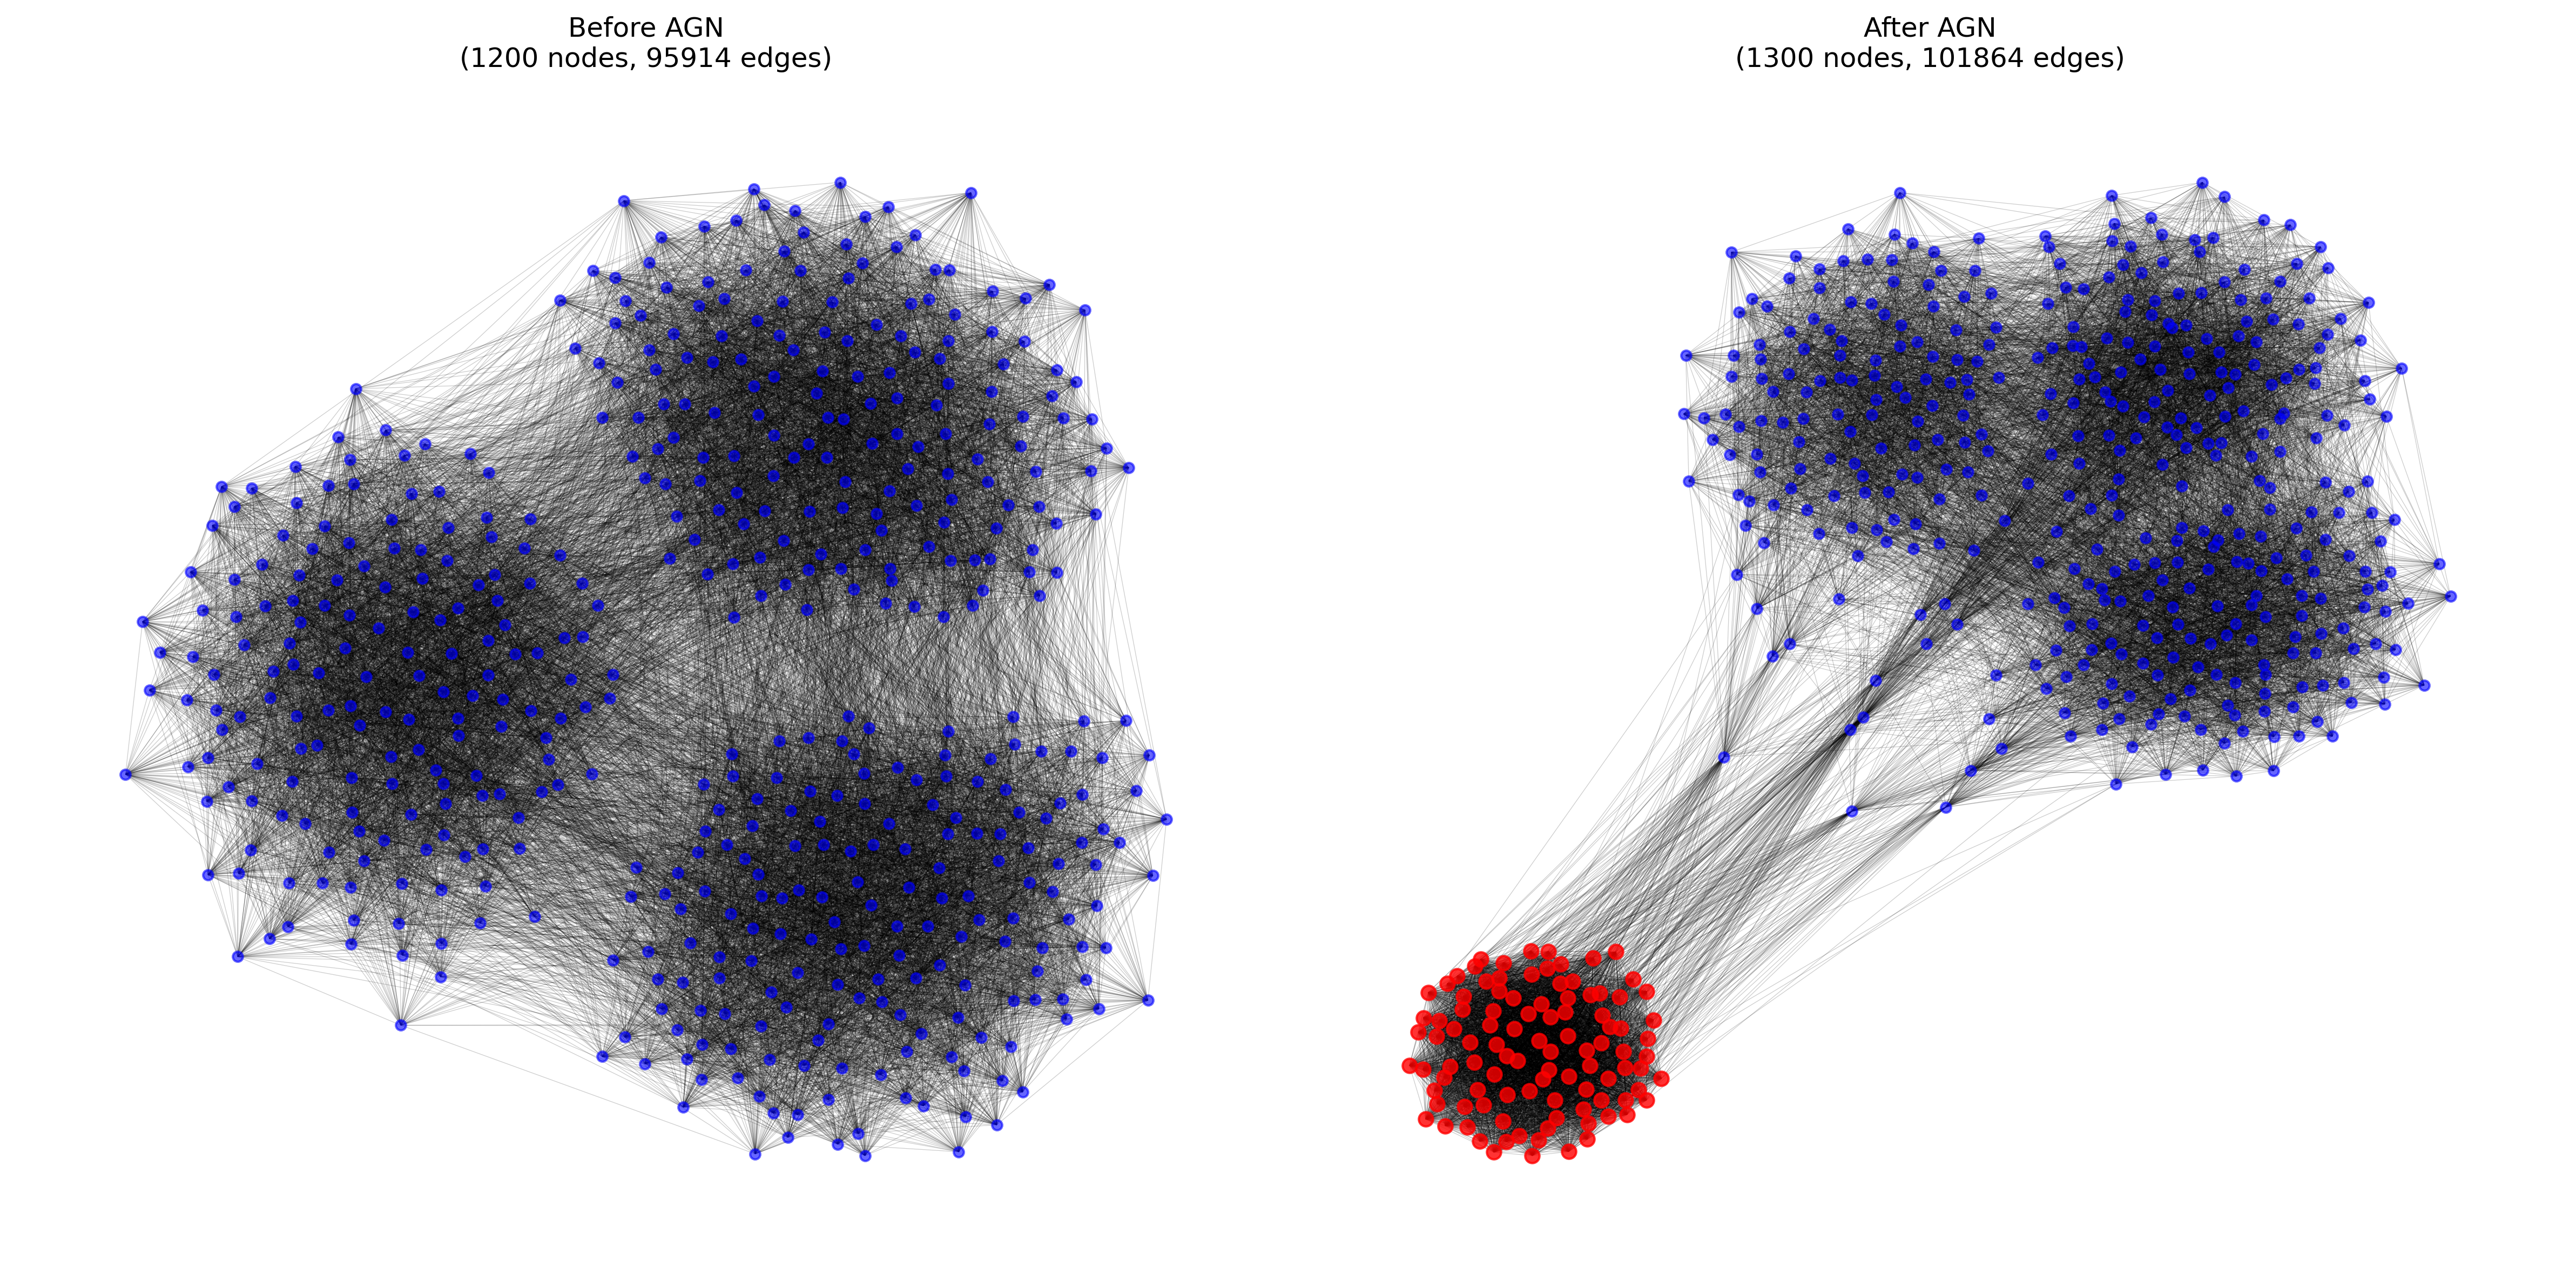
\includegraphics[width=0.32\textwidth]{results/plots/karate_network_comparison.png}
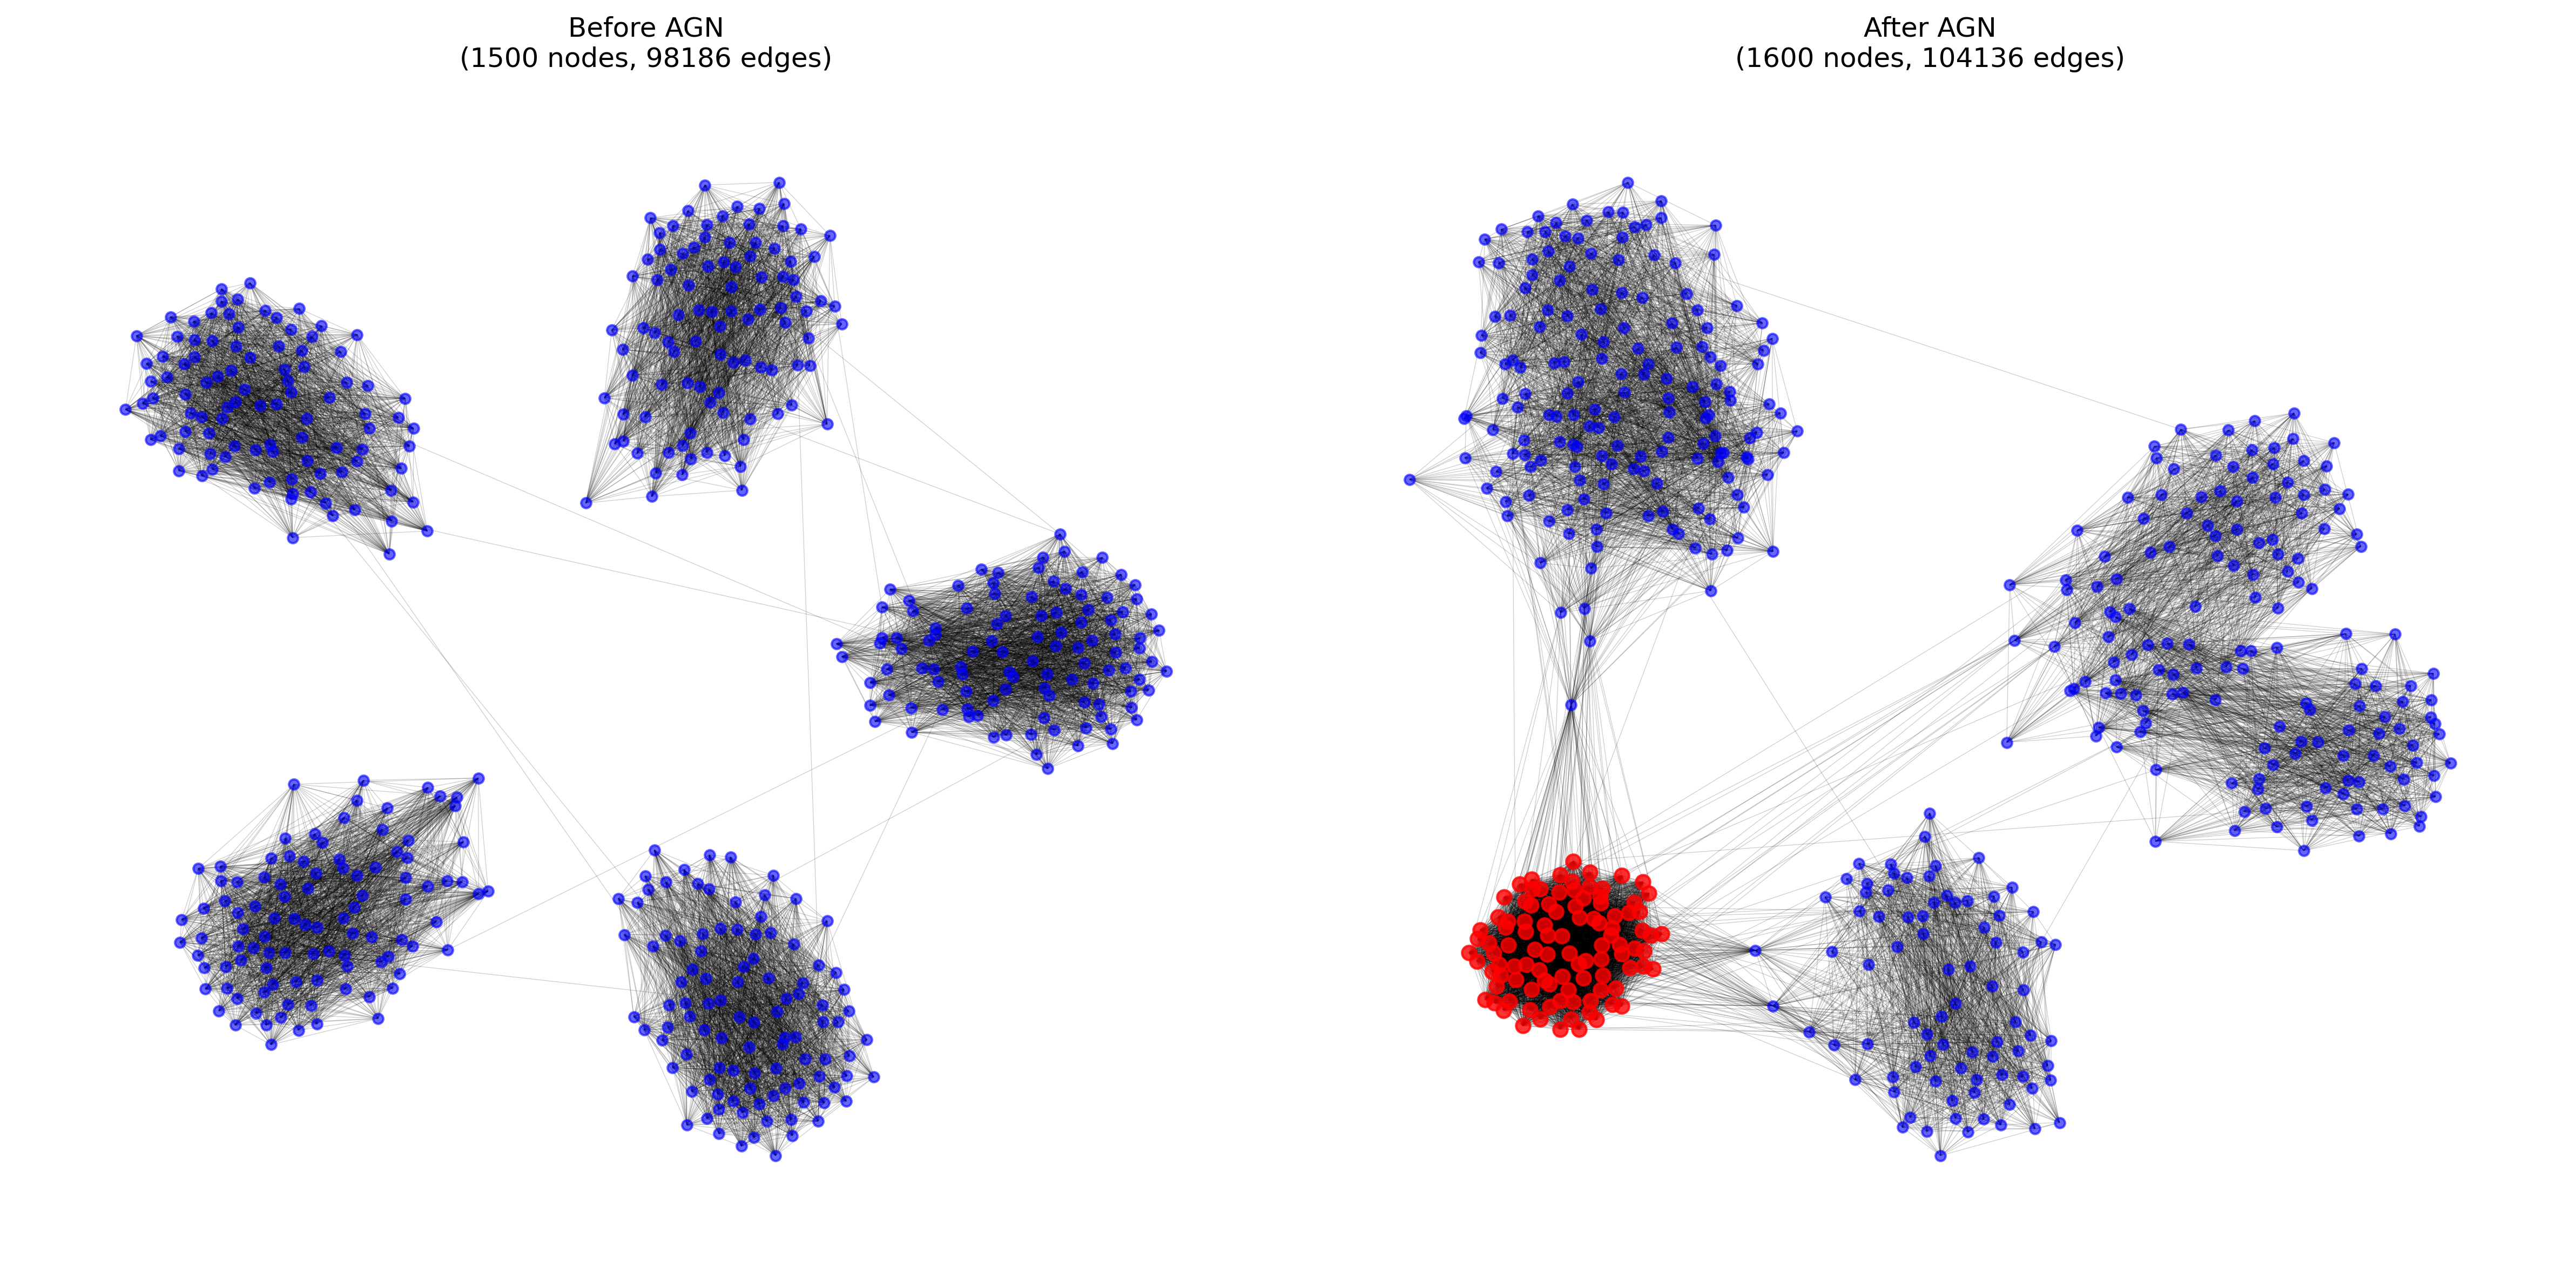
\includegraphics[width=0.32\textwidth]{results/plots/facebook_network_comparison.png}
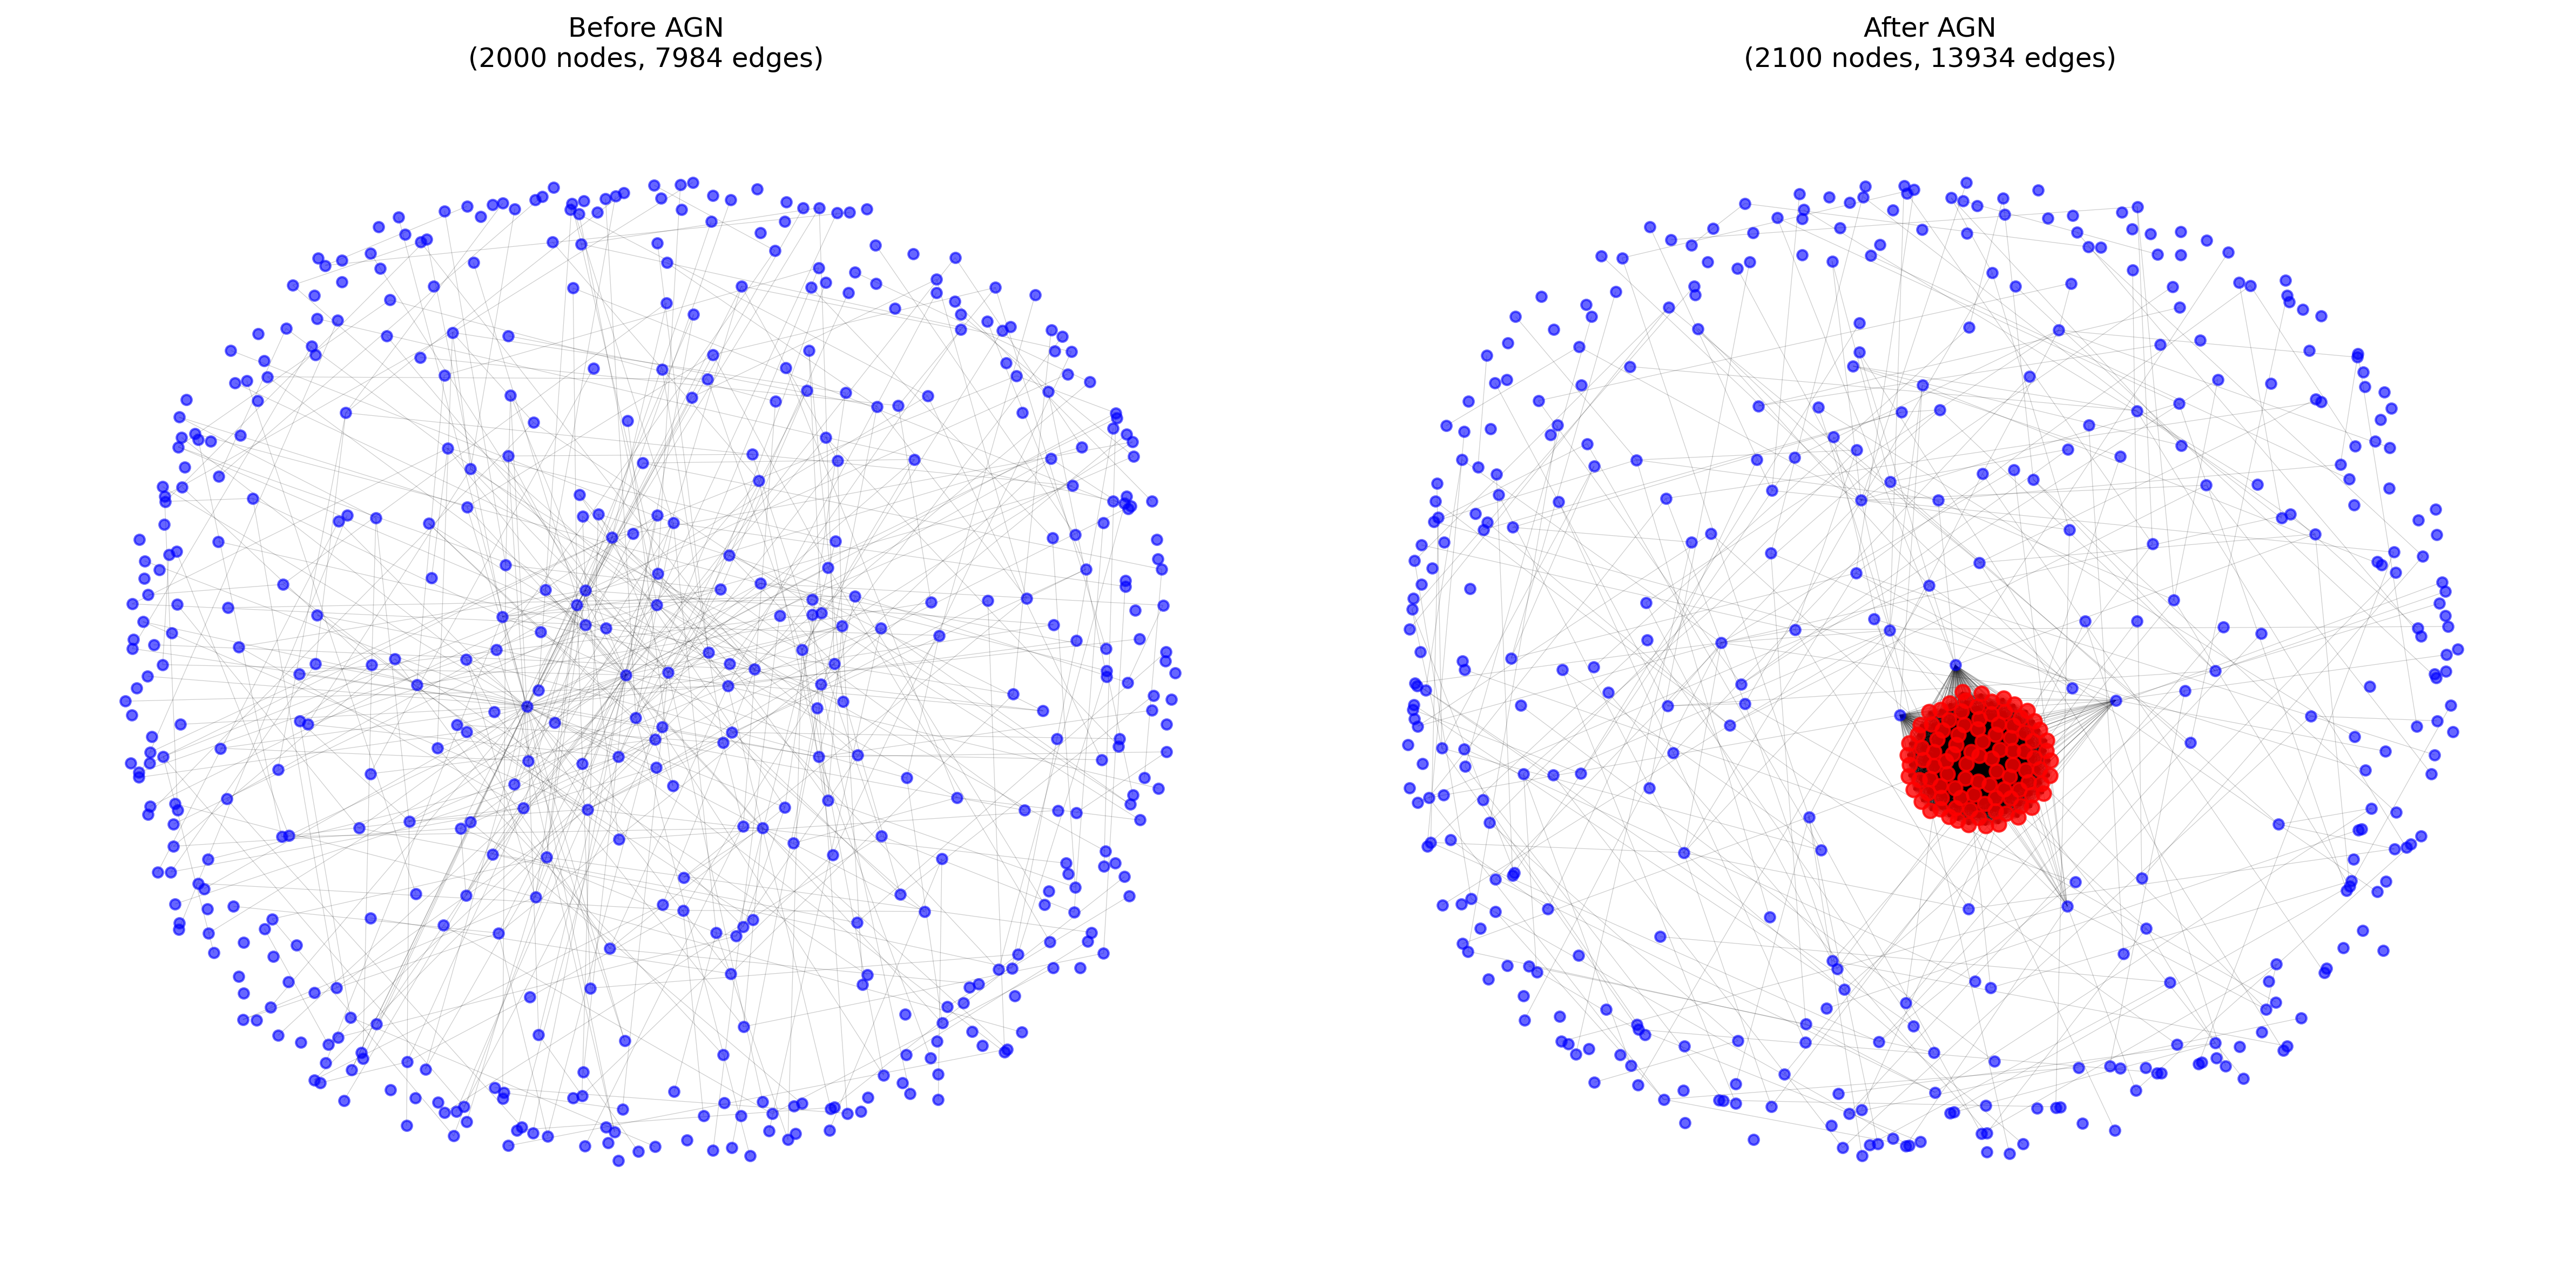
\includegraphics[width=0.32\textwidth]{results/plots/email_network_comparison.png}
\caption{Network structure comparison for (left) Community-SBM, (center) Facebook Ego, and (right) Email Communication networks. Left panels show original networks; right panels show augmented networks with generated nodes highlighted in red. Networks are sampled to 500 nodes for visualization clarity.}
\label{fig:network_comparison}
\end{figure}

Figure~\ref{fig:metrics_comparison} shows normalized bar chart comparisons of key network metrics before and after node insertion. The visualizations demonstrate consistent preservation of network properties across all datasets, with metric changes that adapt to initial network characteristics. Density changes are most pronounced in the Email Network due to its sparse initial state, while clustering increases are observed across all datasets, indicating enhanced local connectivity.

\begin{figure}[h]
\centering
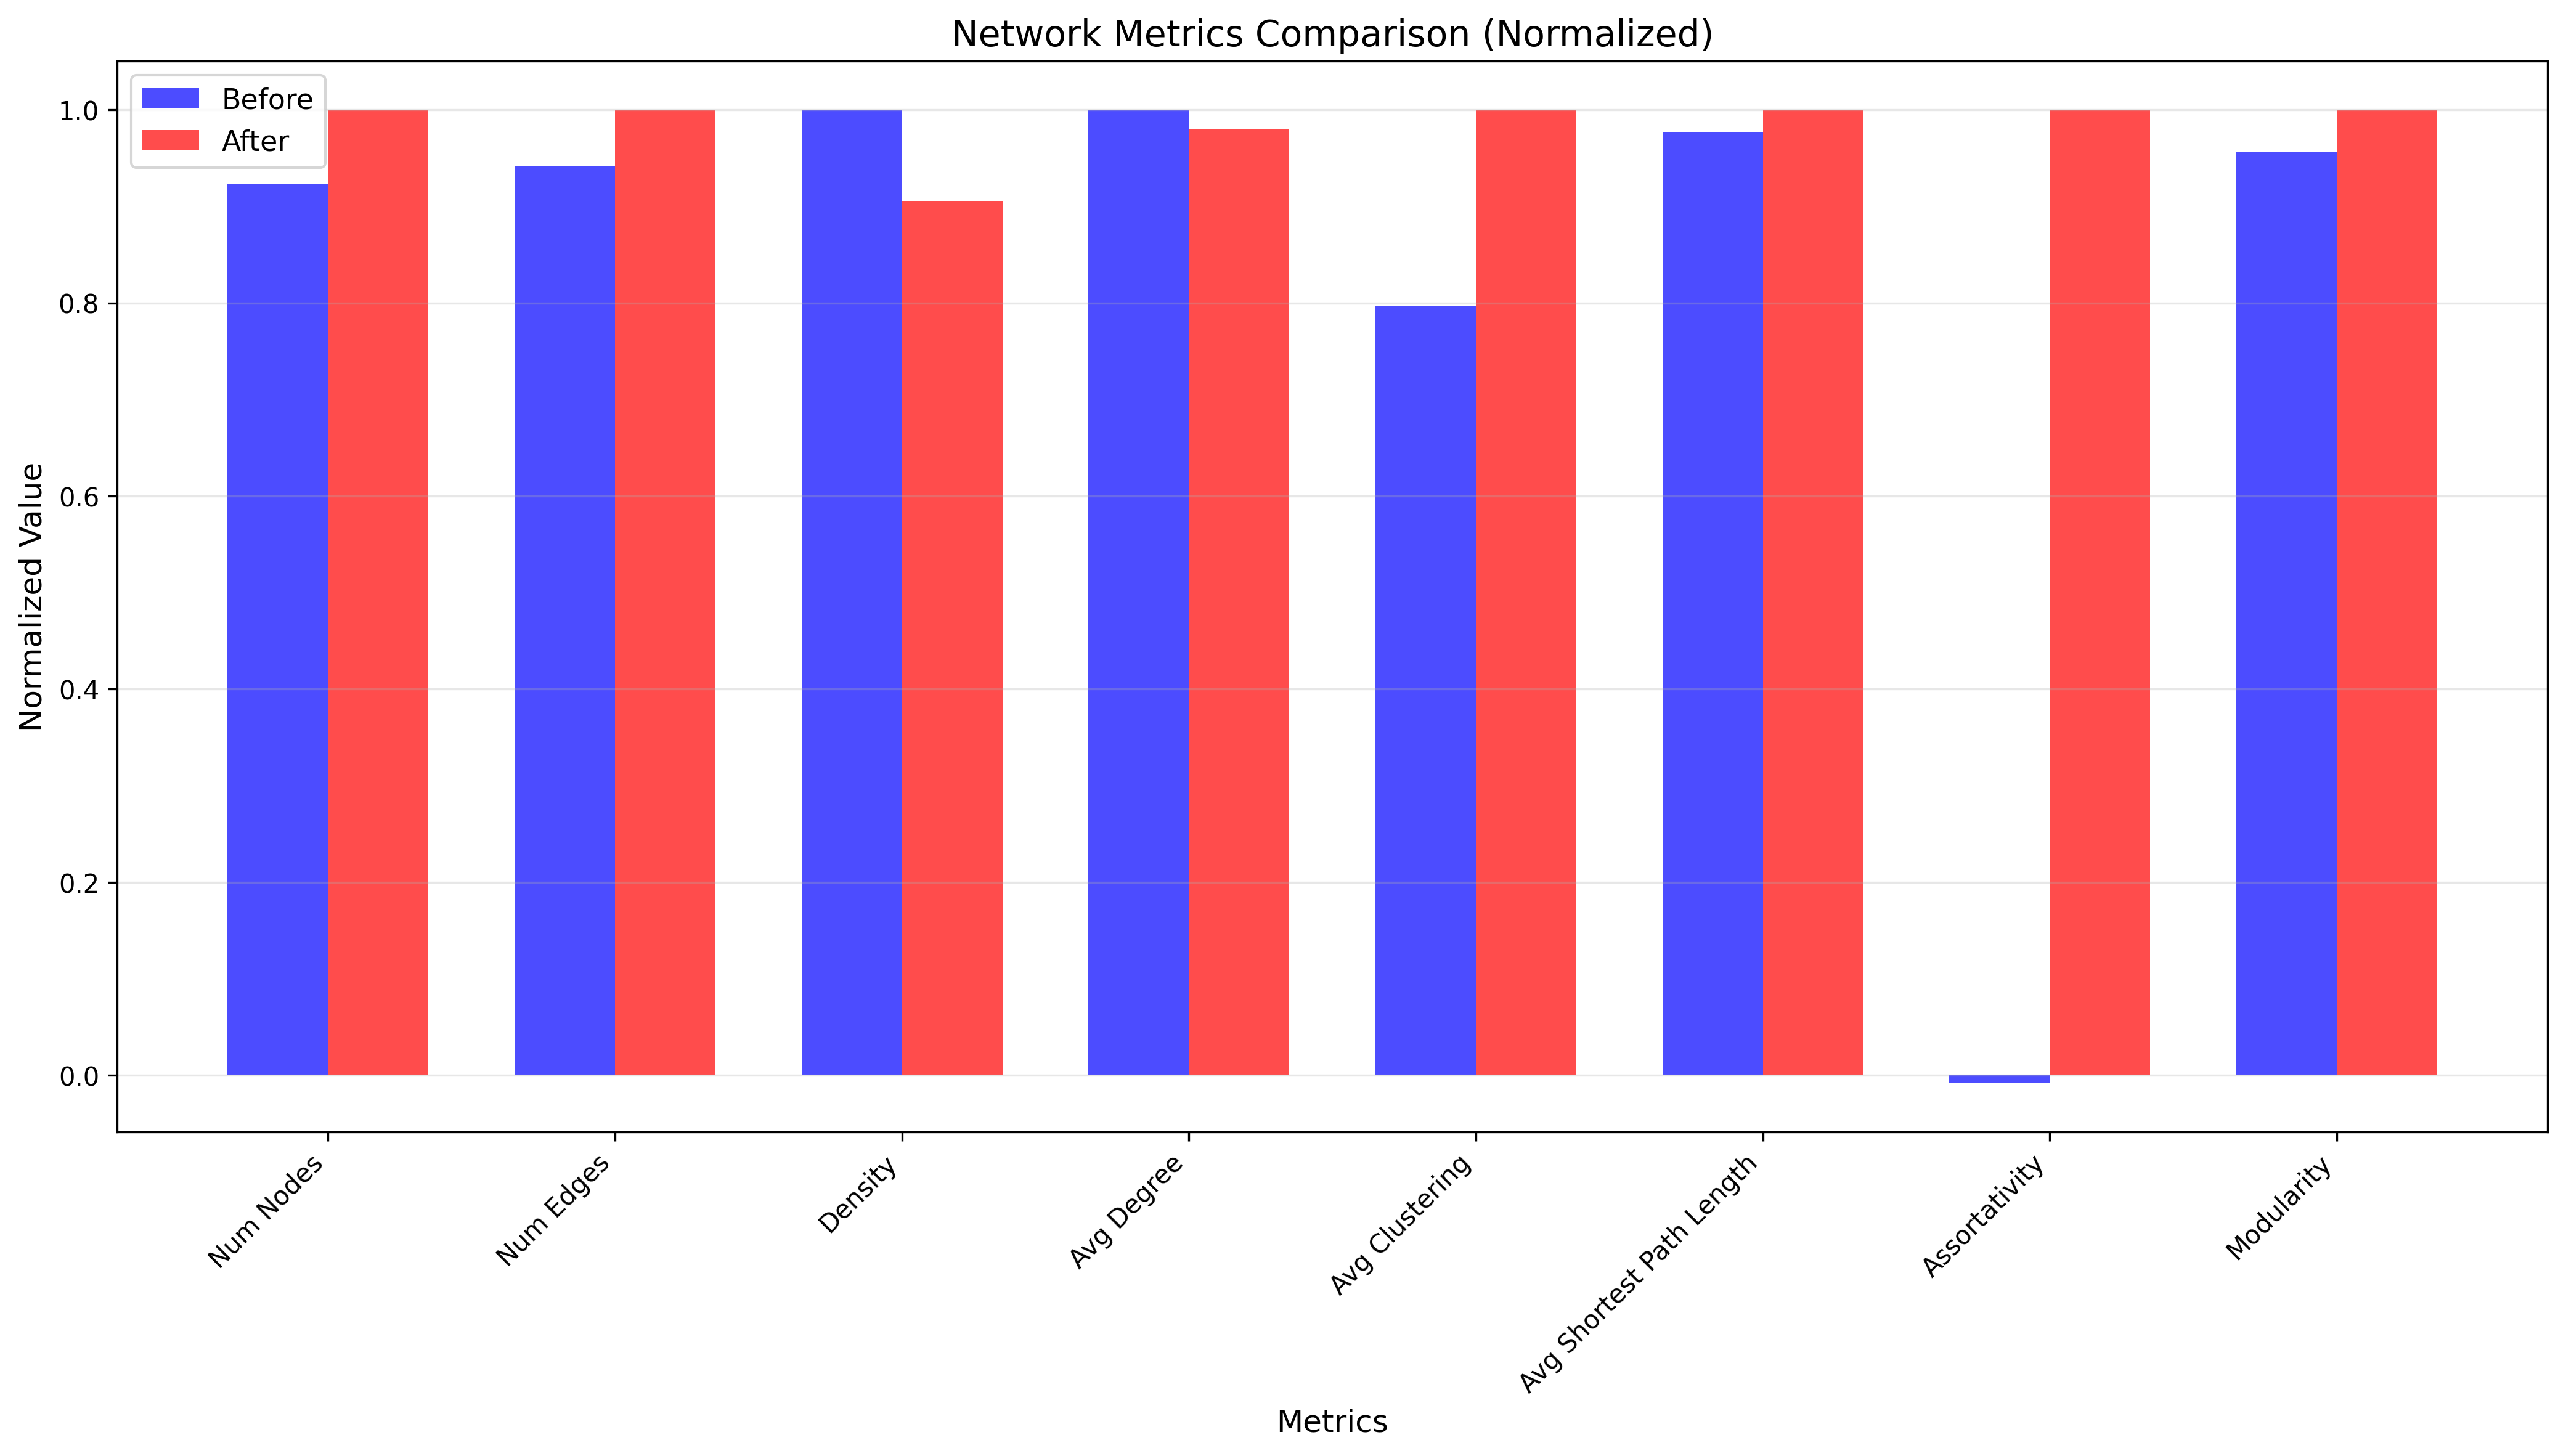
\includegraphics[width=0.32\textwidth]{results/plots/karate_metrics_comparison.png}
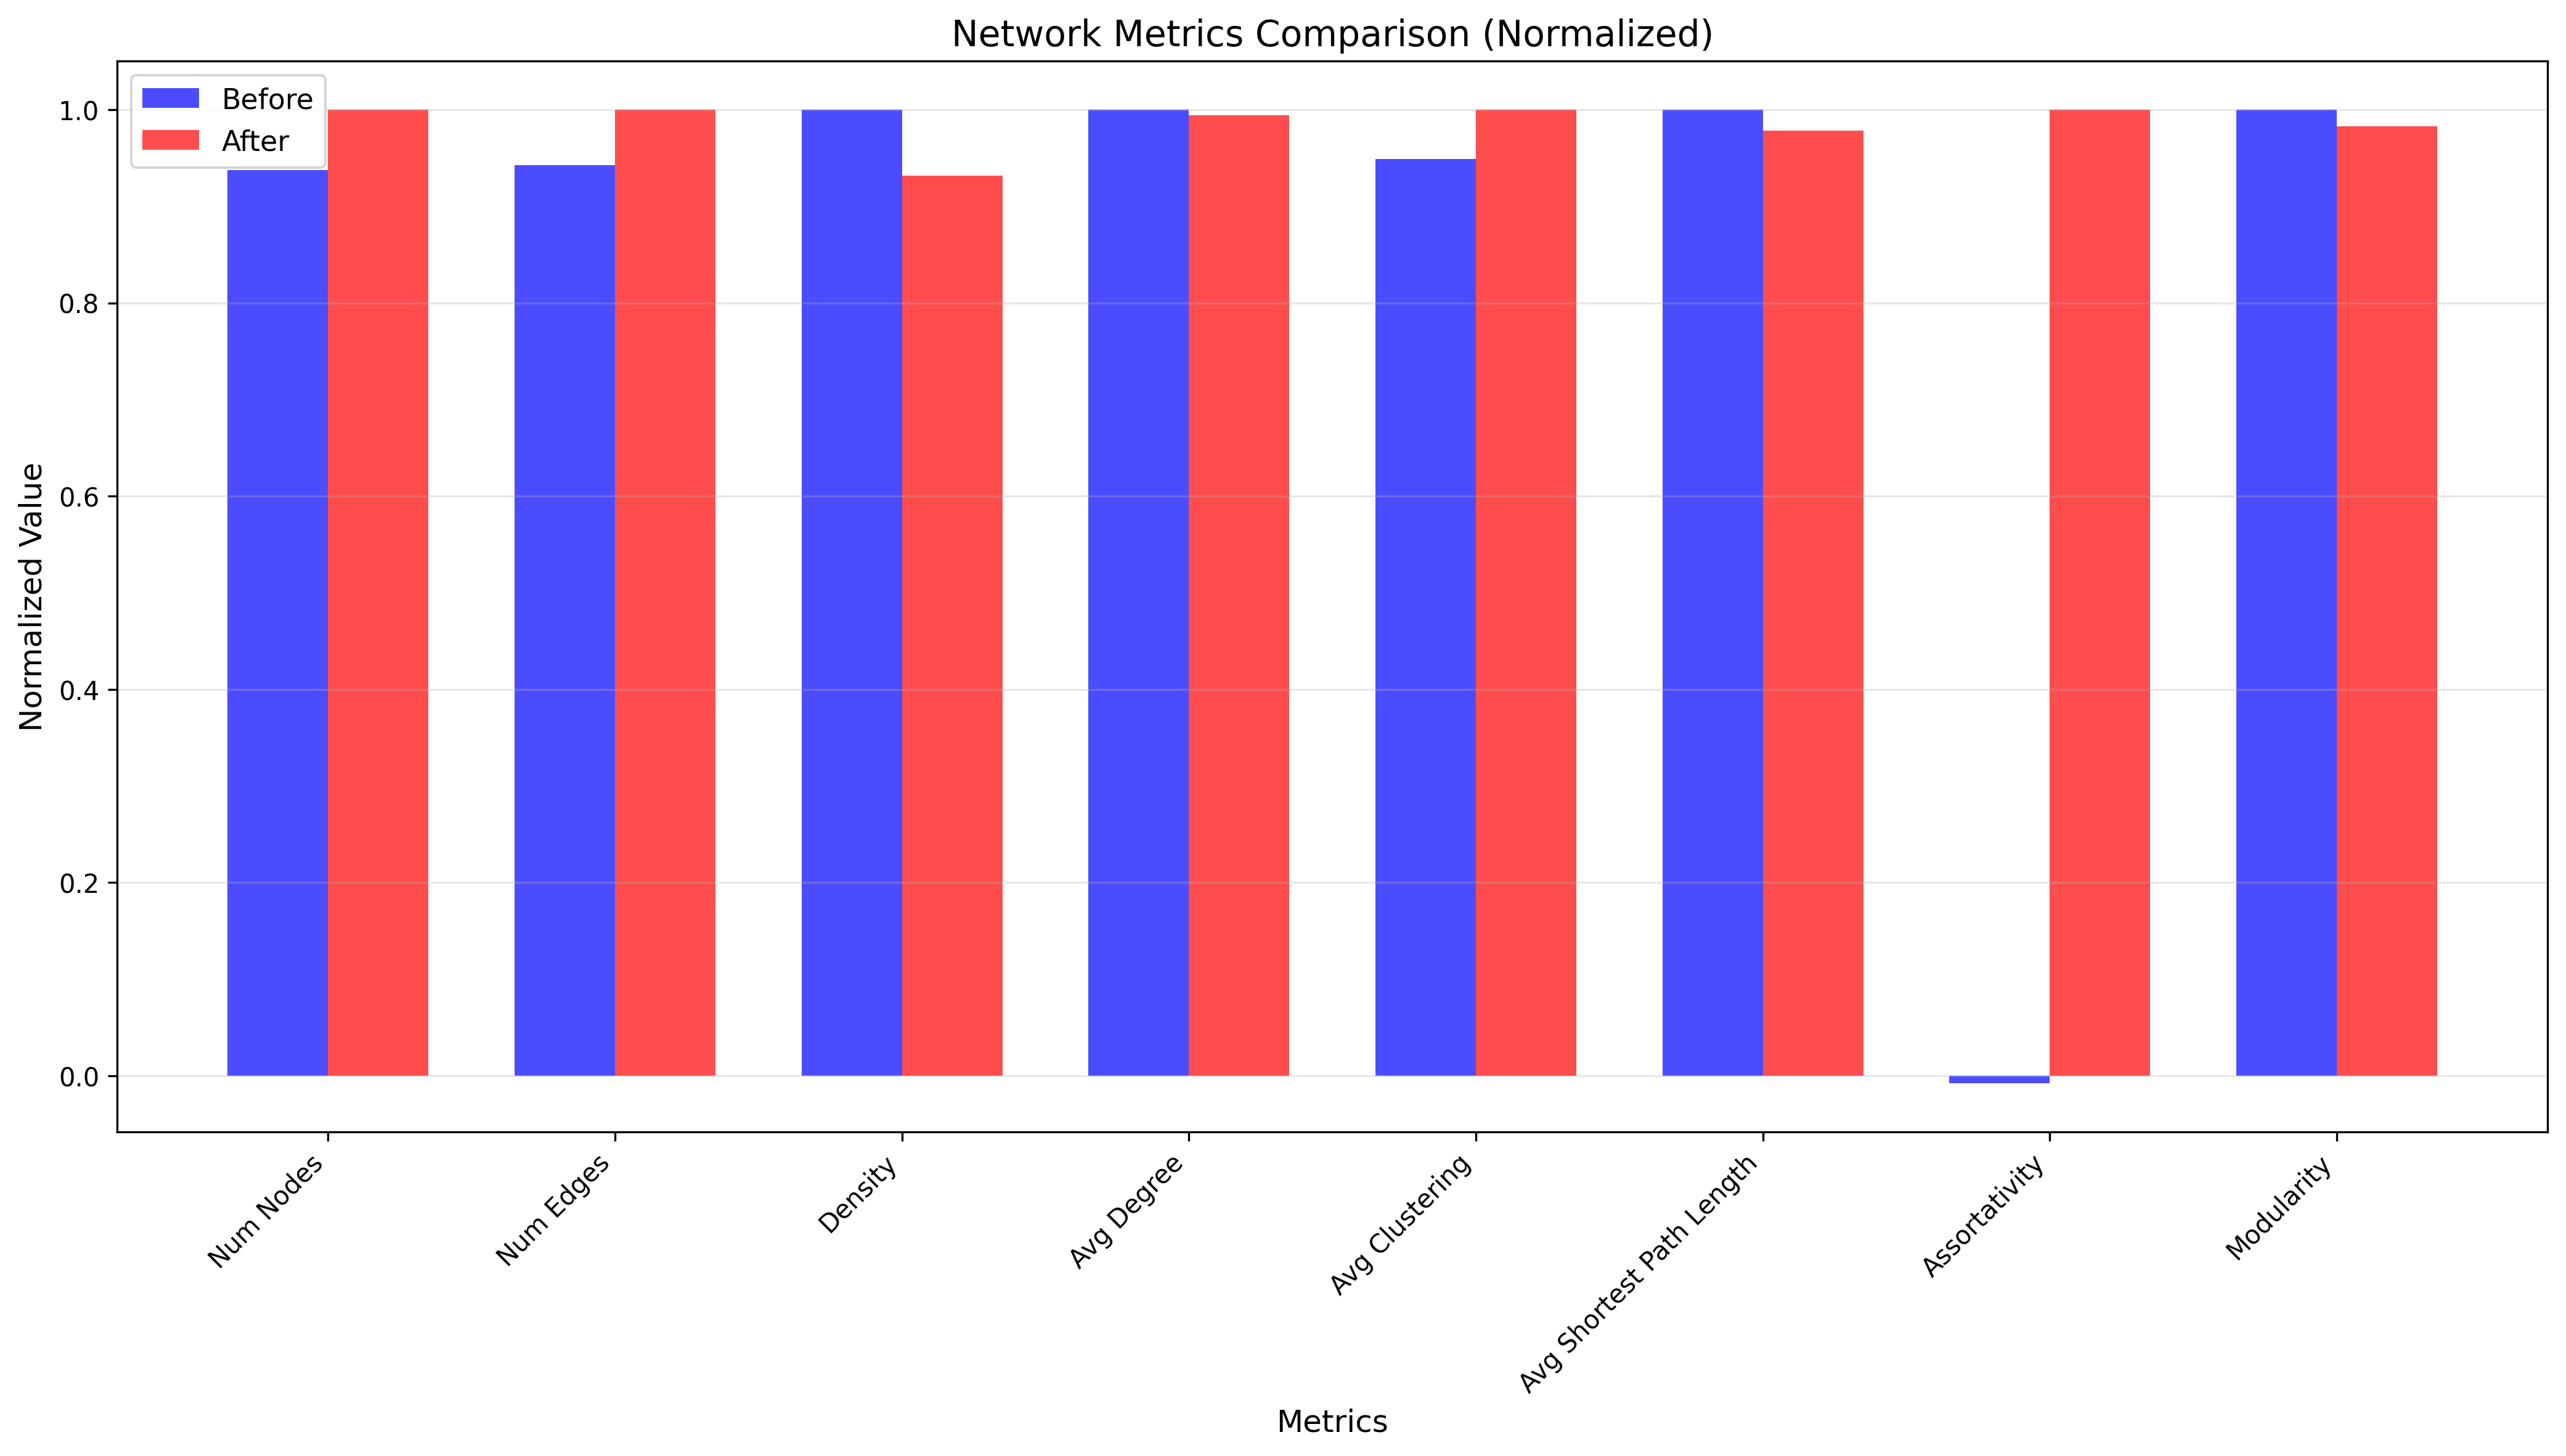
\includegraphics[width=0.32\textwidth]{results/plots/facebook_metrics_comparison.png}
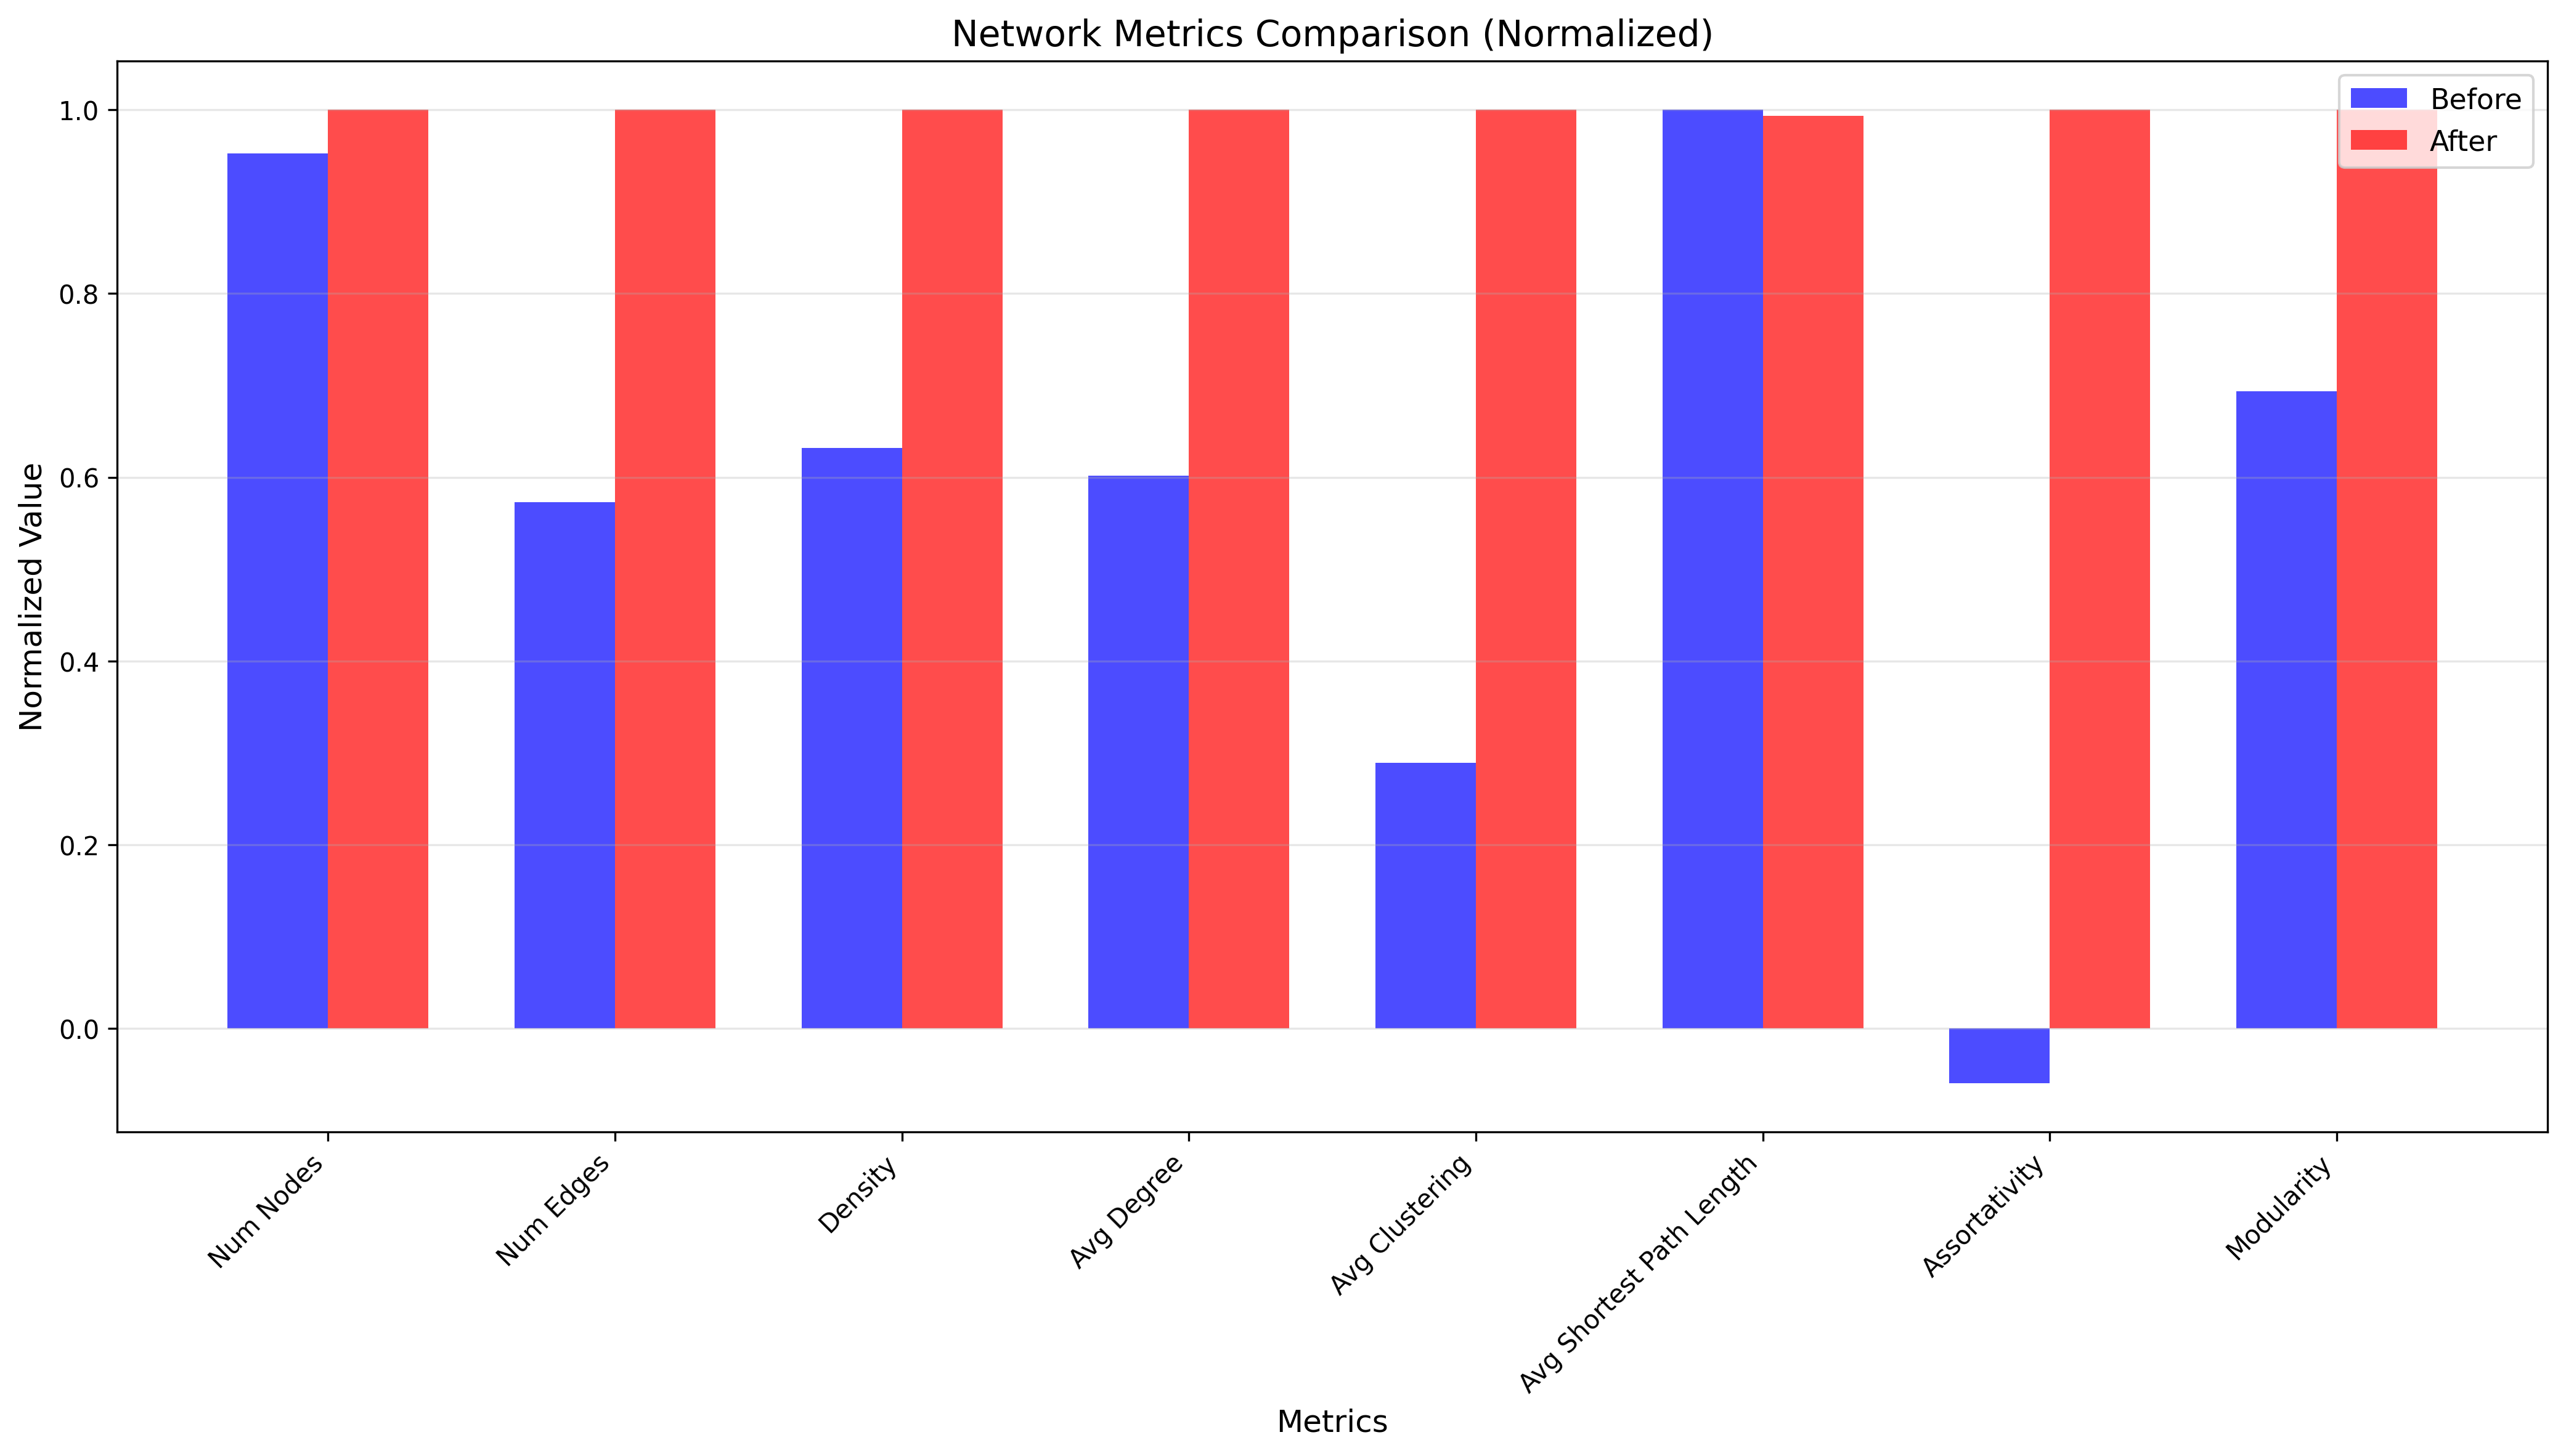
\includegraphics[width=0.32\textwidth]{results/plots/email_metrics_comparison.png}
\caption{Normalized metrics comparison for (left) Community-SBM, (center) Facebook Ego, and (right) Email Communication networks. Blue bars represent original networks; red bars represent augmented networks. Metrics are normalized by their maximum absolute values for visualization.}
\label{fig:metrics_comparison}
\end{figure}

\subsection{Degree Distribution Analysis}

Figure~\ref{fig:degree_dist} shows degree distributions before and after node insertion for all three datasets. All datasets maintain similar degree distribution shapes, with generated nodes exhibiting degrees consistent with existing nodes. The Community-SBM network shows stable degree distributions with slight rightward shift, indicating generated nodes connect with moderate degrees that fit the existing distribution. The Facebook Ego network maintains its degree distribution shape, demonstrating preservation of community-based connectivity patterns. The Email Network shows the most variation, with generated nodes filling gaps in the degree distribution, consistent with its sparse initial state and demonstrating AGN's ability to enhance connectivity in scale-free networks while preserving the power-law structure.

\begin{figure}[h]
\centering
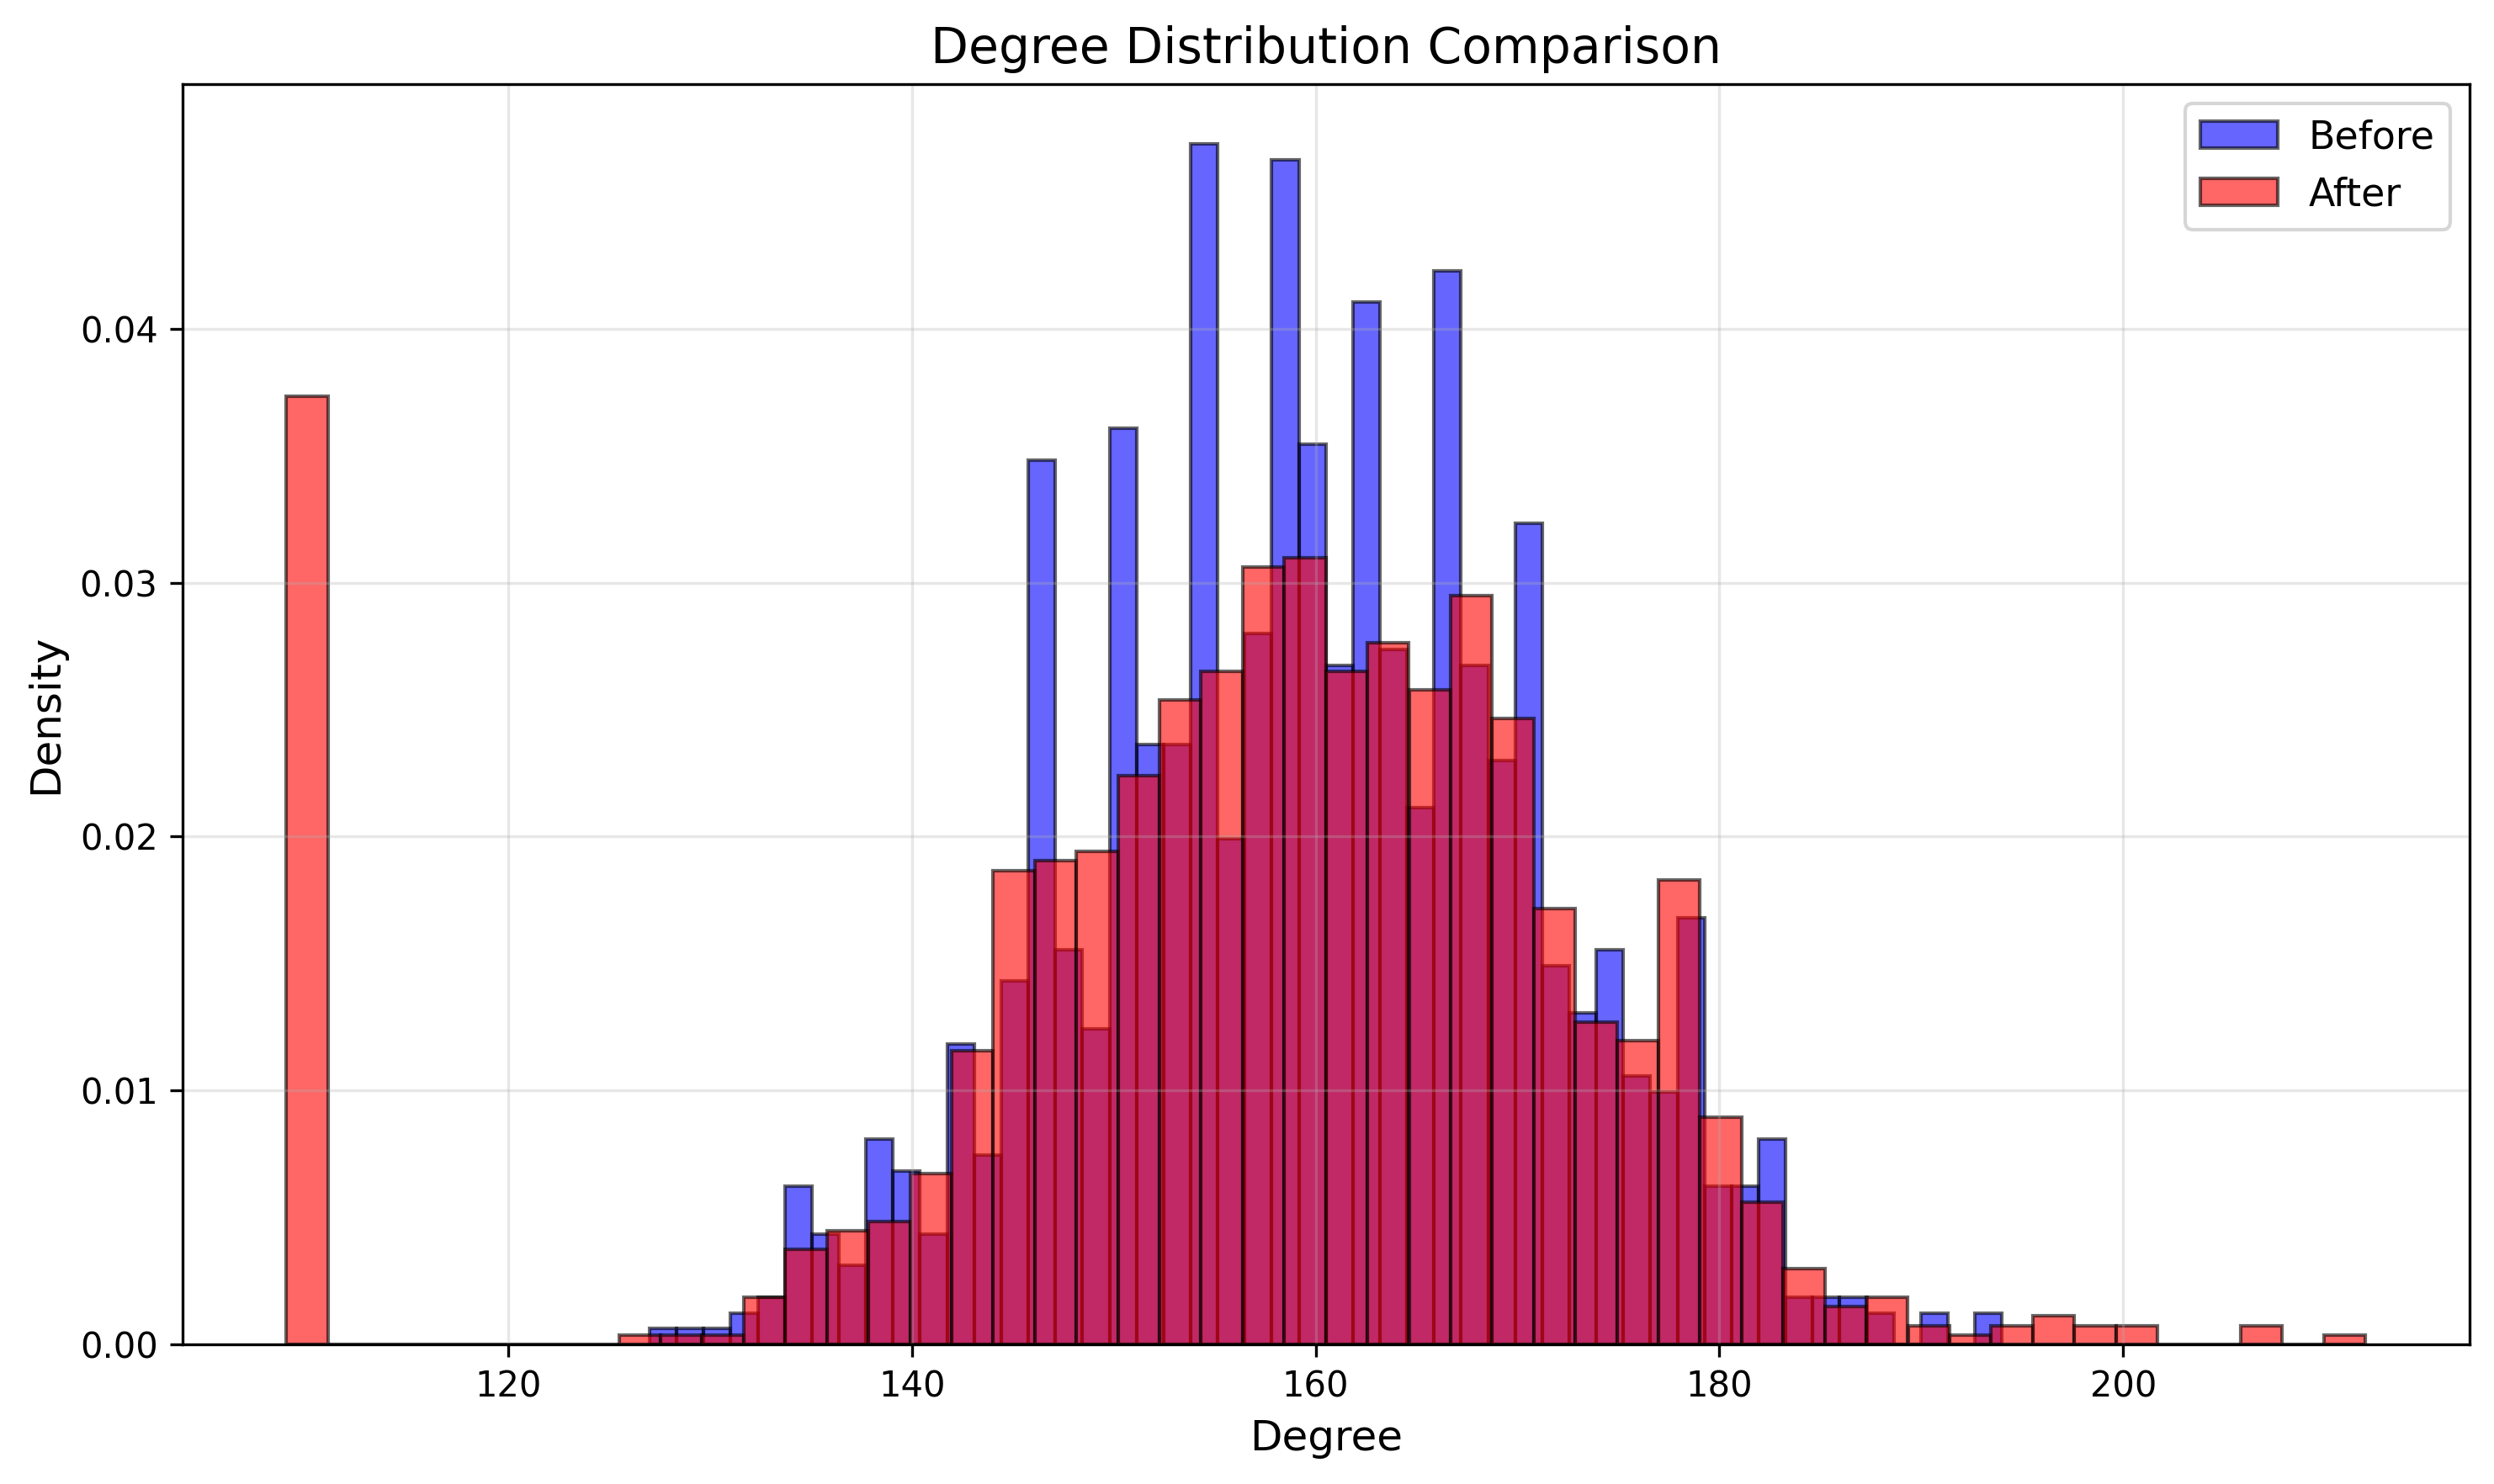
\includegraphics[width=0.32\textwidth]{results/plots/karate_degree_distribution.png}
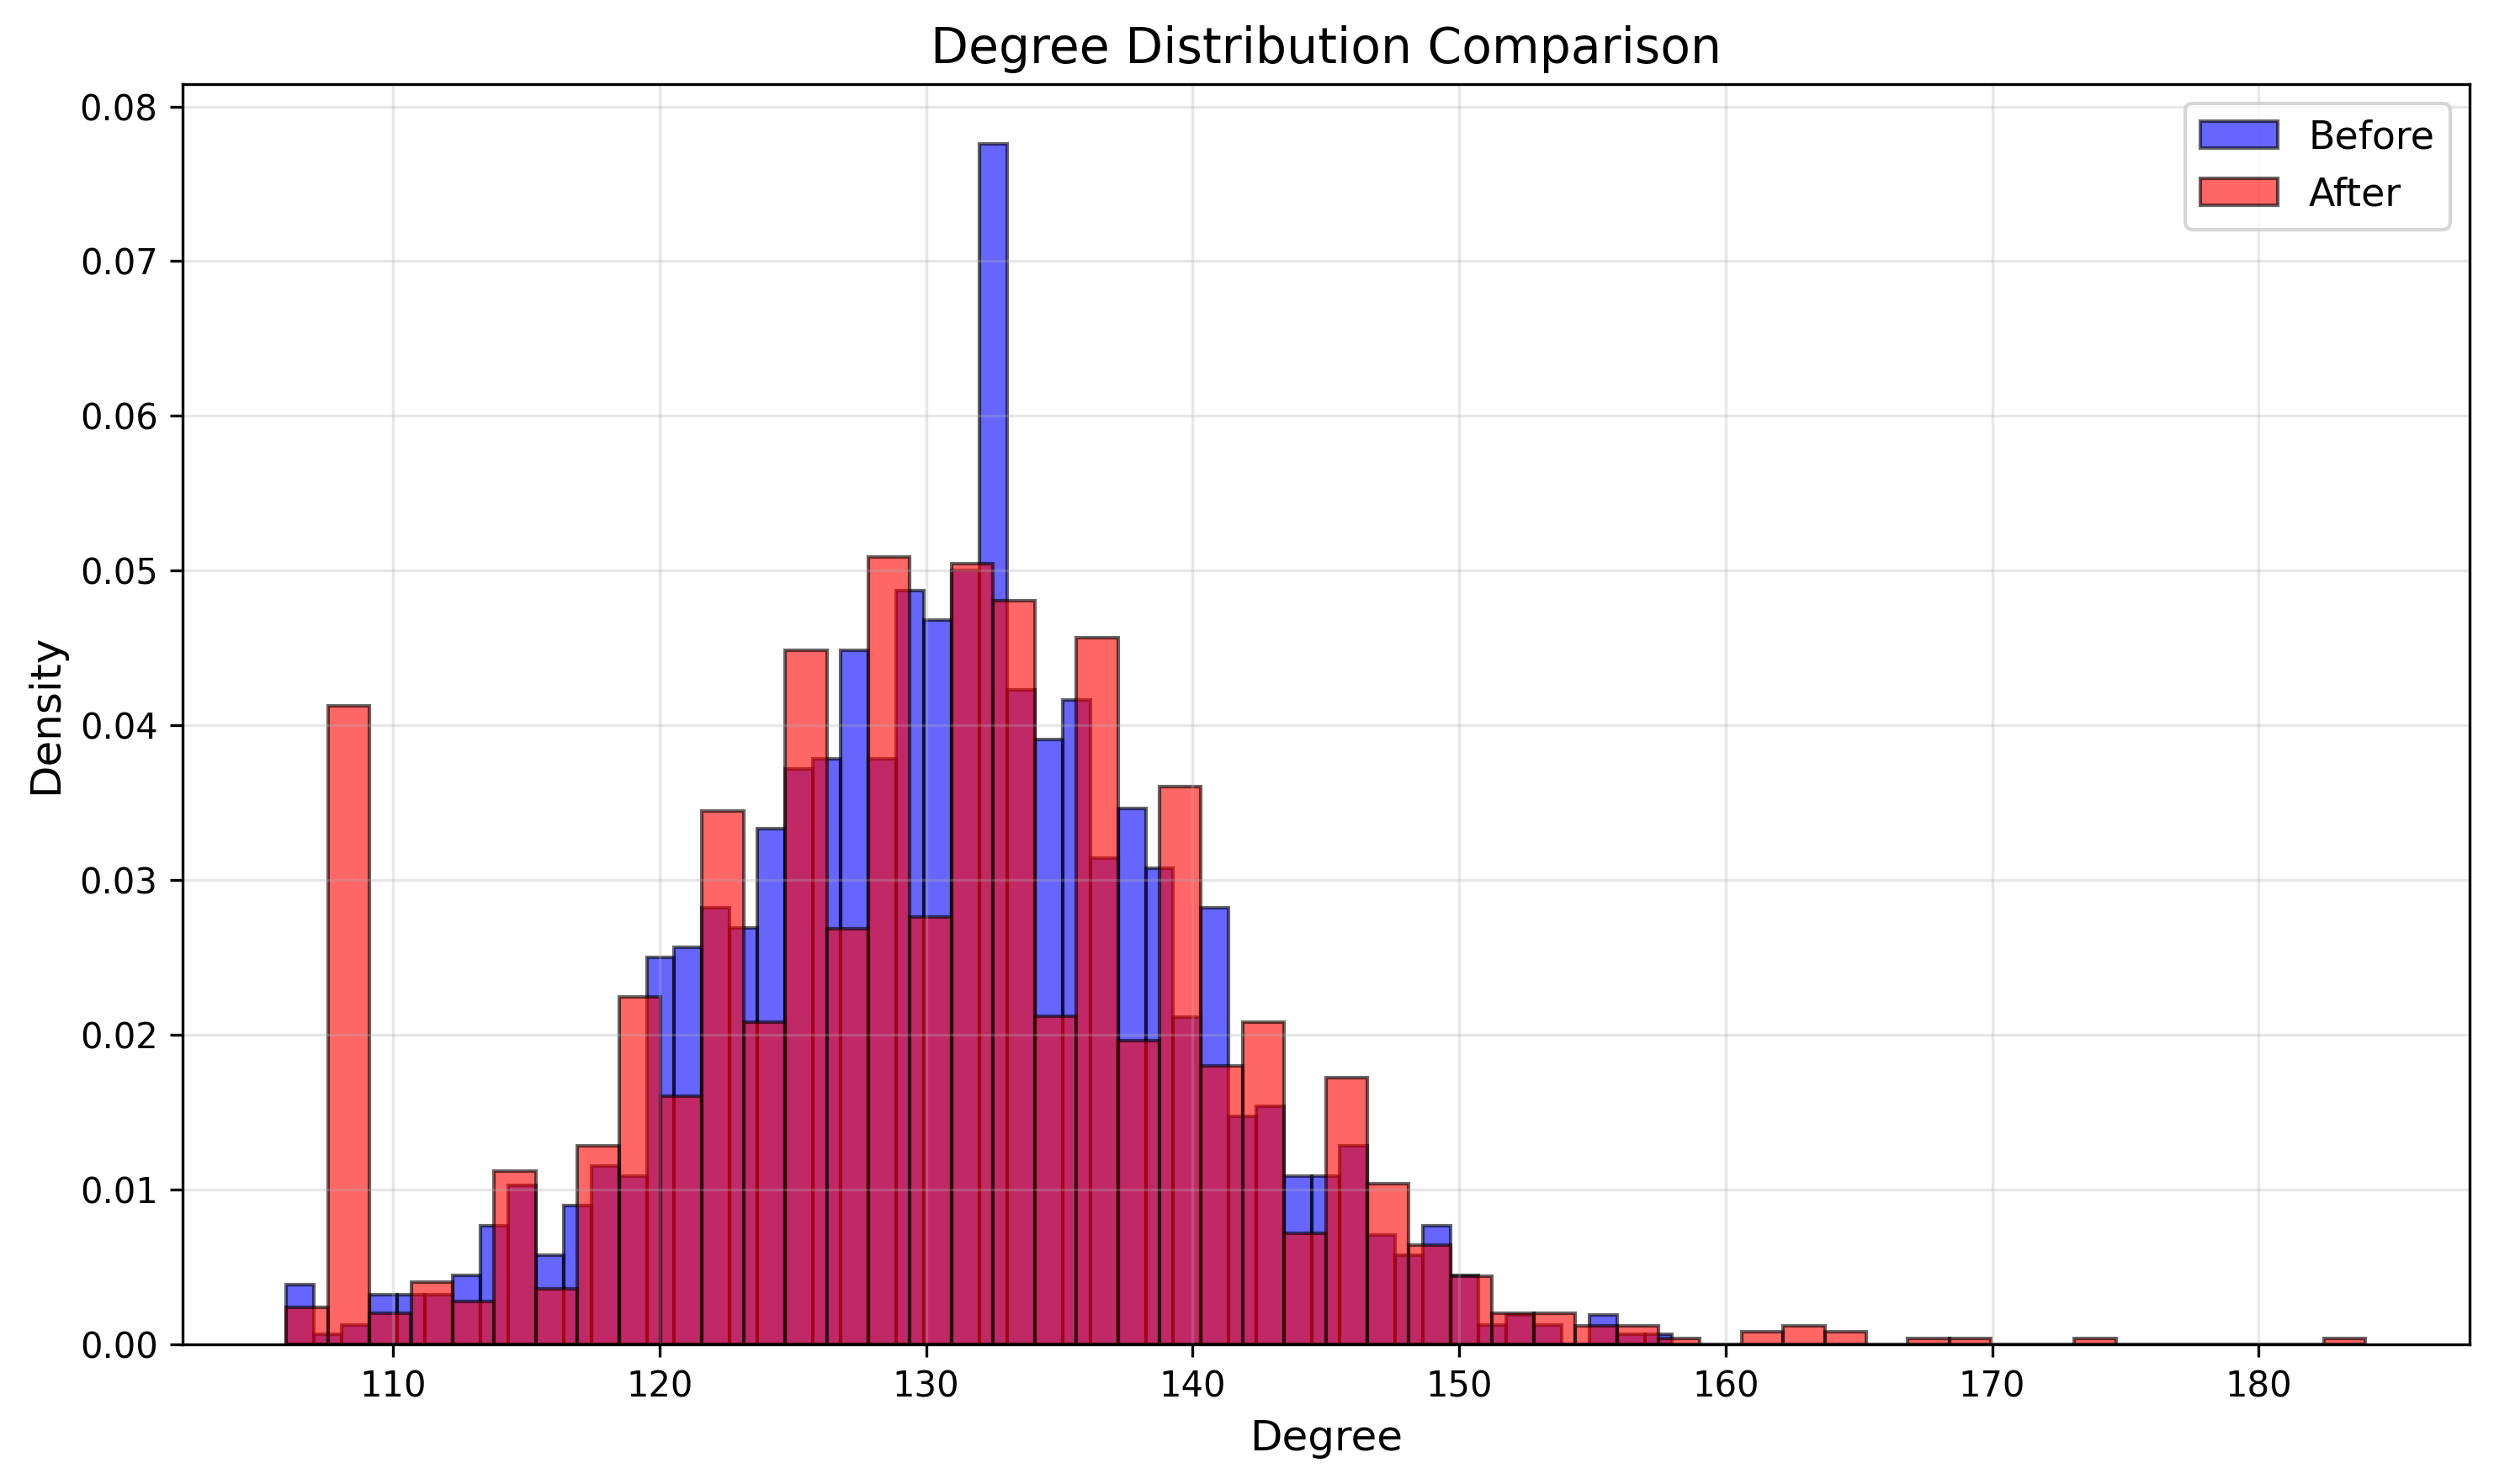
\includegraphics[width=0.32\textwidth]{results/plots/facebook_degree_distribution.png}
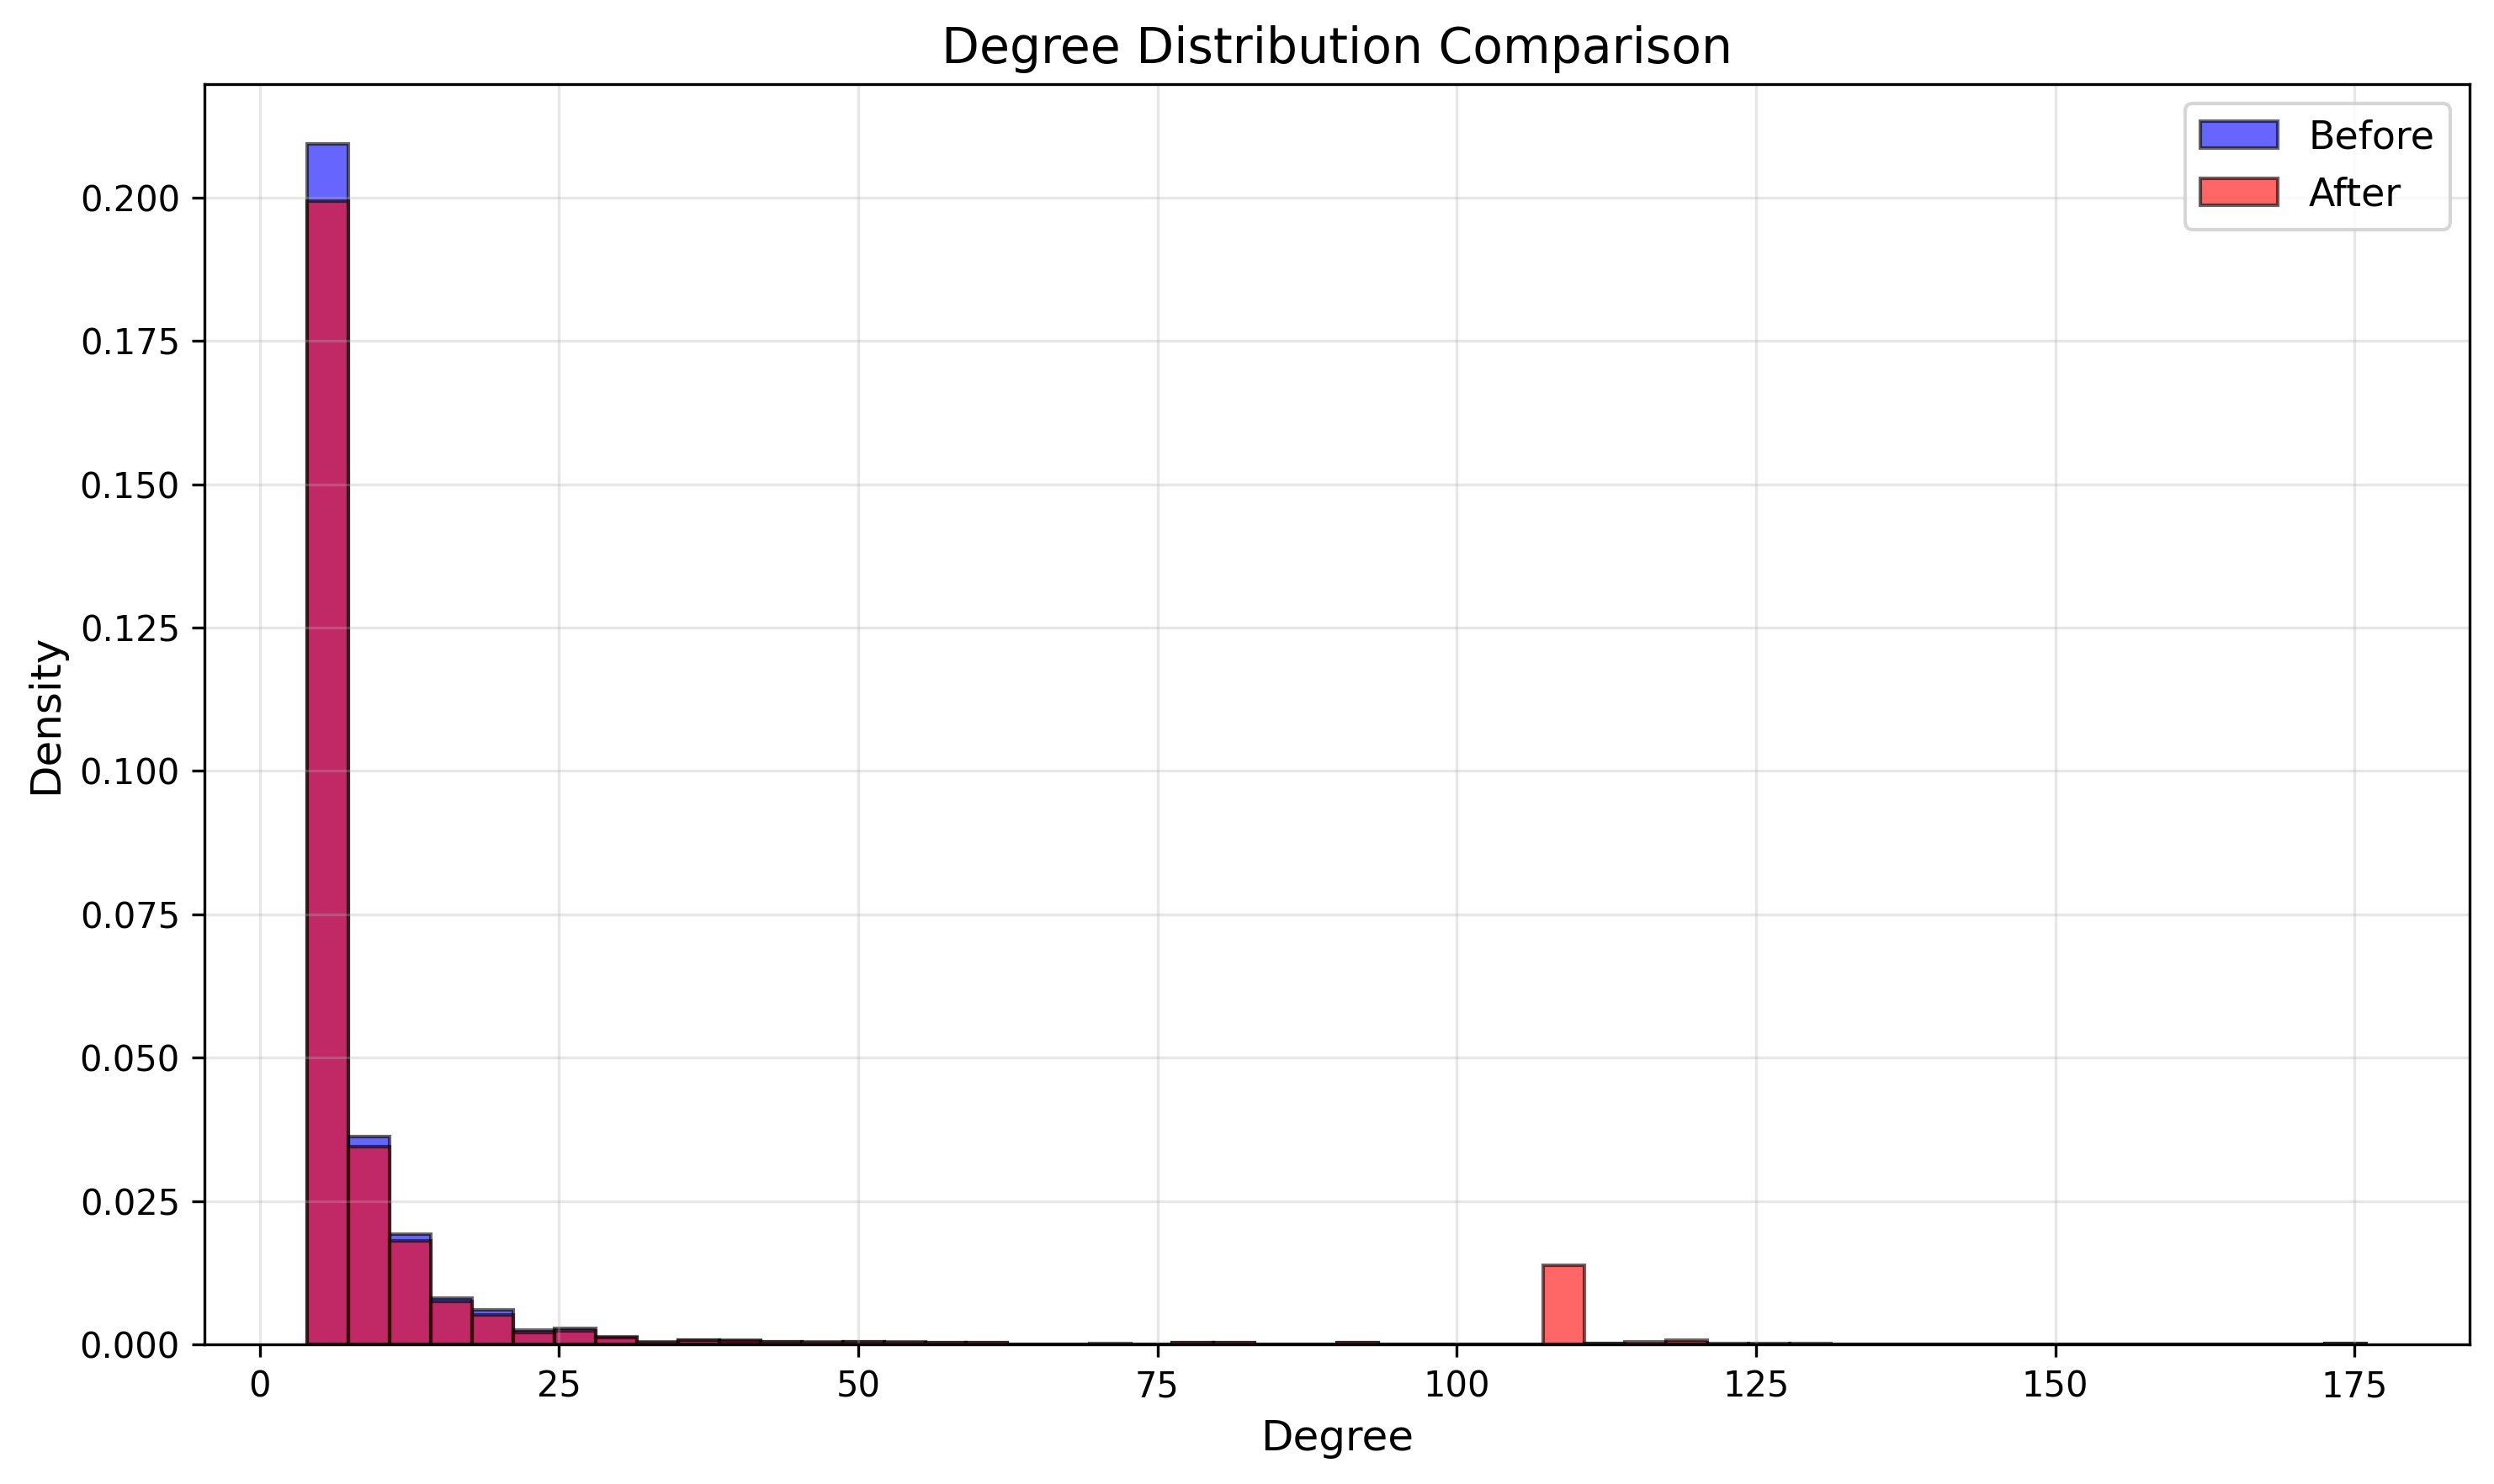
\includegraphics[width=0.32\textwidth]{results/plots/email_degree_distribution.png}
\caption{Degree distribution comparisons for (left) Community-SBM, (center) Facebook Ego, and (right) Email Communication networks. Blue histograms represent original networks, red histograms represent augmented networks after AGN node insertion. Distributions are normalized to density for comparison.}
\label{fig:degree_dist}
\end{figure}

\subsection{Novelty Analysis}

Table~\ref{tab:novelty} presents novelty statistics for generated nodes. The novelty classification uses a threshold-based definition: nodes with minimum distance to original nodes above the 25th percentile are classified as novel, which results in exactly 75\% of nodes being novel by construction. This consistent threshold enables fair comparison across datasets, but the key insight lies in the distributional properties rather than the percentage itself.

\begin{table}[h]
\centering
\caption{Novelty Analysis}
\label{tab:novelty}
\begin{tabular}{lccc}
\toprule
Metric & Community-SBM & Facebook Ego & Email Network \\
\midrule
Avg min distance to original & 0.000285 & 0.001436 & 0.075649 \\
Avg mean distance to original & 0.0370 & 0.0269 & 0.3707 \\
Novelty percentage (\%) & 75.0 & 75.0 & 75.0 \\
\bottomrule
\end{tabular}
\end{table}

The Email Network shows substantially higher distances to original nodes (mean distance 0.3707 vs. 0.0370-0.0269, Table~\ref{tab:novelty}), reflecting its sparser feature space where nodes are naturally more dispersed. The Community-SBM network shows the smallest distances (mean 0.0370), consistent with its dense community structure where nodes share similar features. The Facebook Ego network shows intermediate distances (mean 0.0269), reflecting its multi-community structure with moderate feature diversity. These distributional differences demonstrate that AGN adapts to different feature spaces while maintaining consistent generation quality. The fact that all datasets achieve the same 75\% threshold-based novelty rate indicates that AGN generates nodes with sufficient diversity relative to each dataset's feature distribution, rather than memorizing existing patterns.

\begin{figure}[h]
\centering
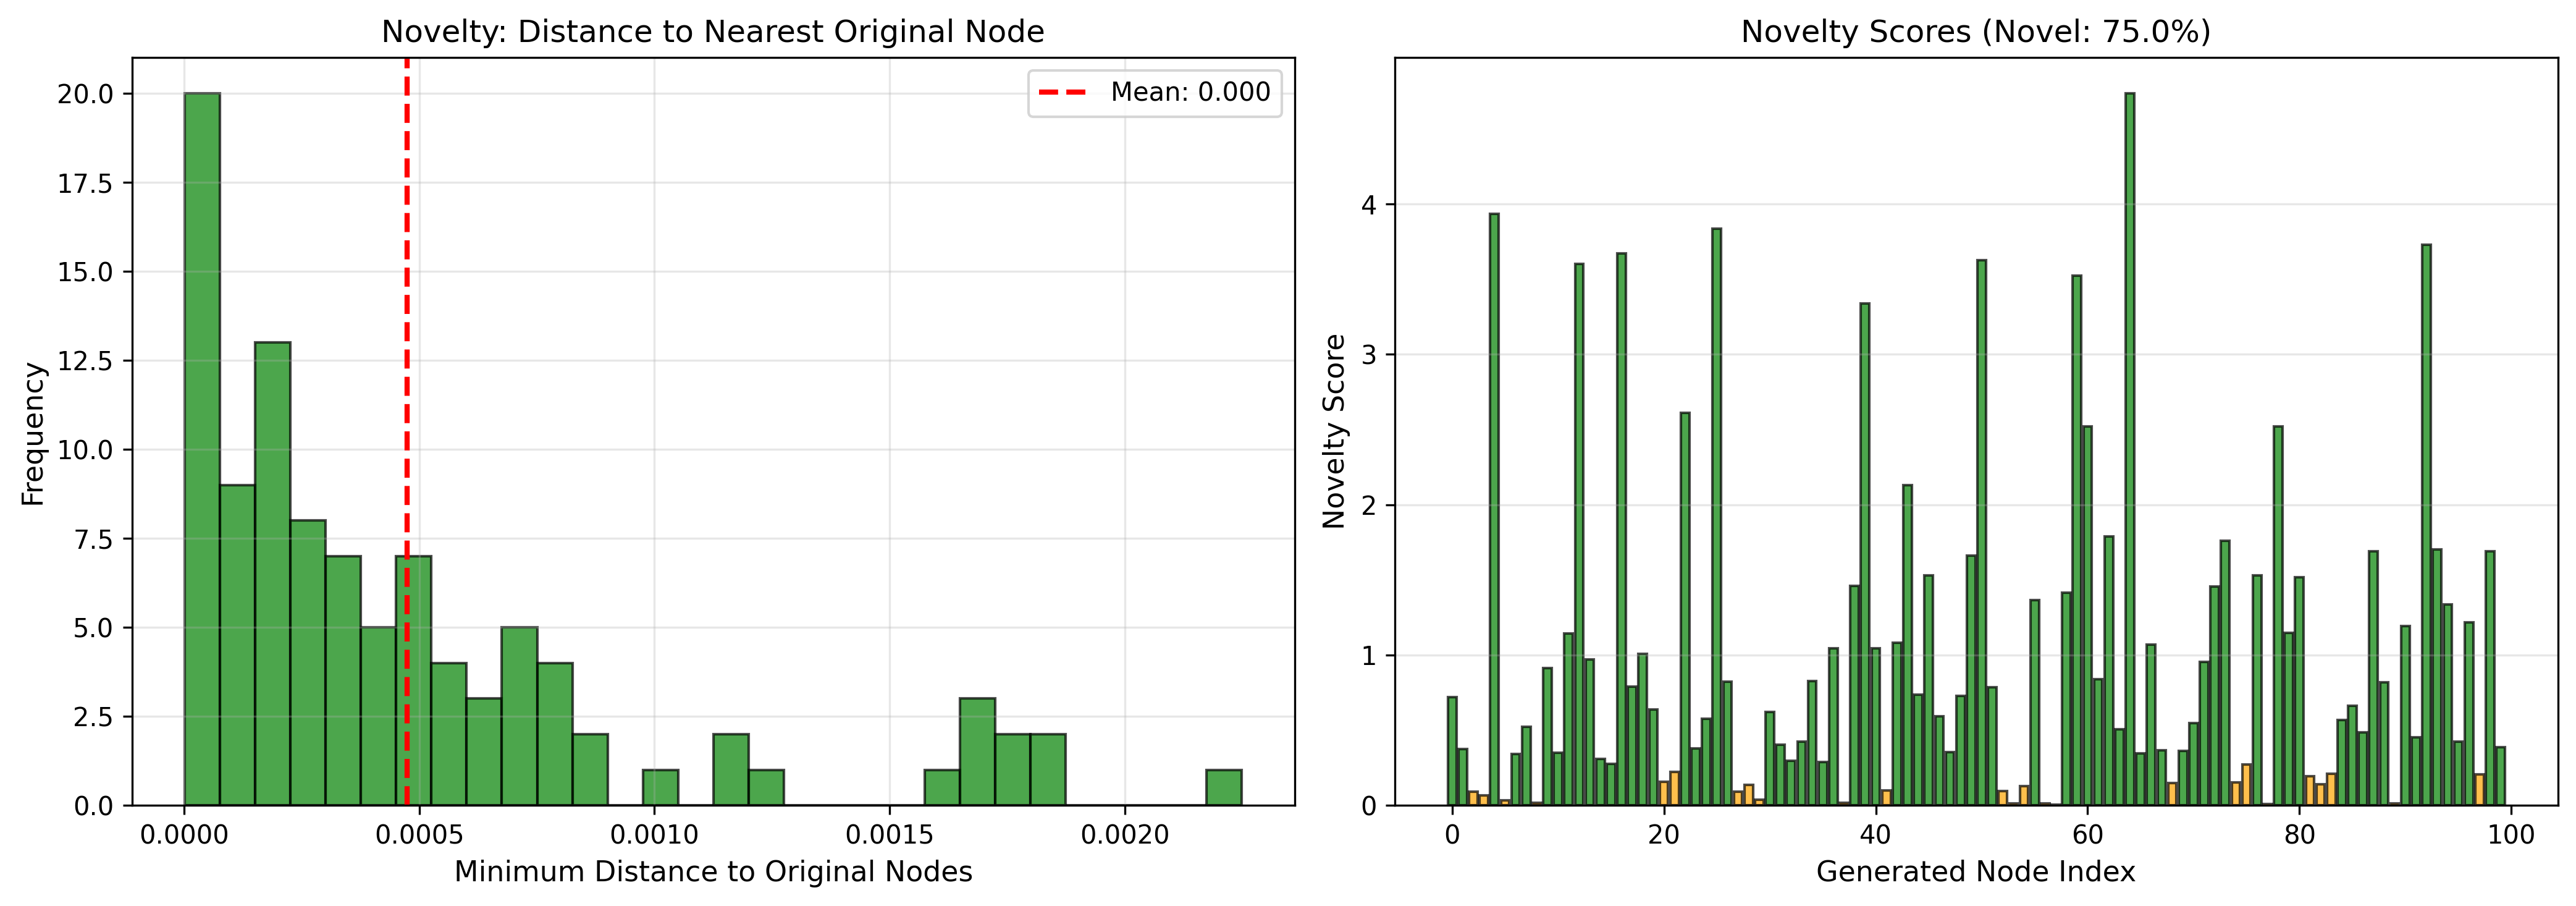
\includegraphics[width=0.32\textwidth]{results/plots/karate_novelty.png}
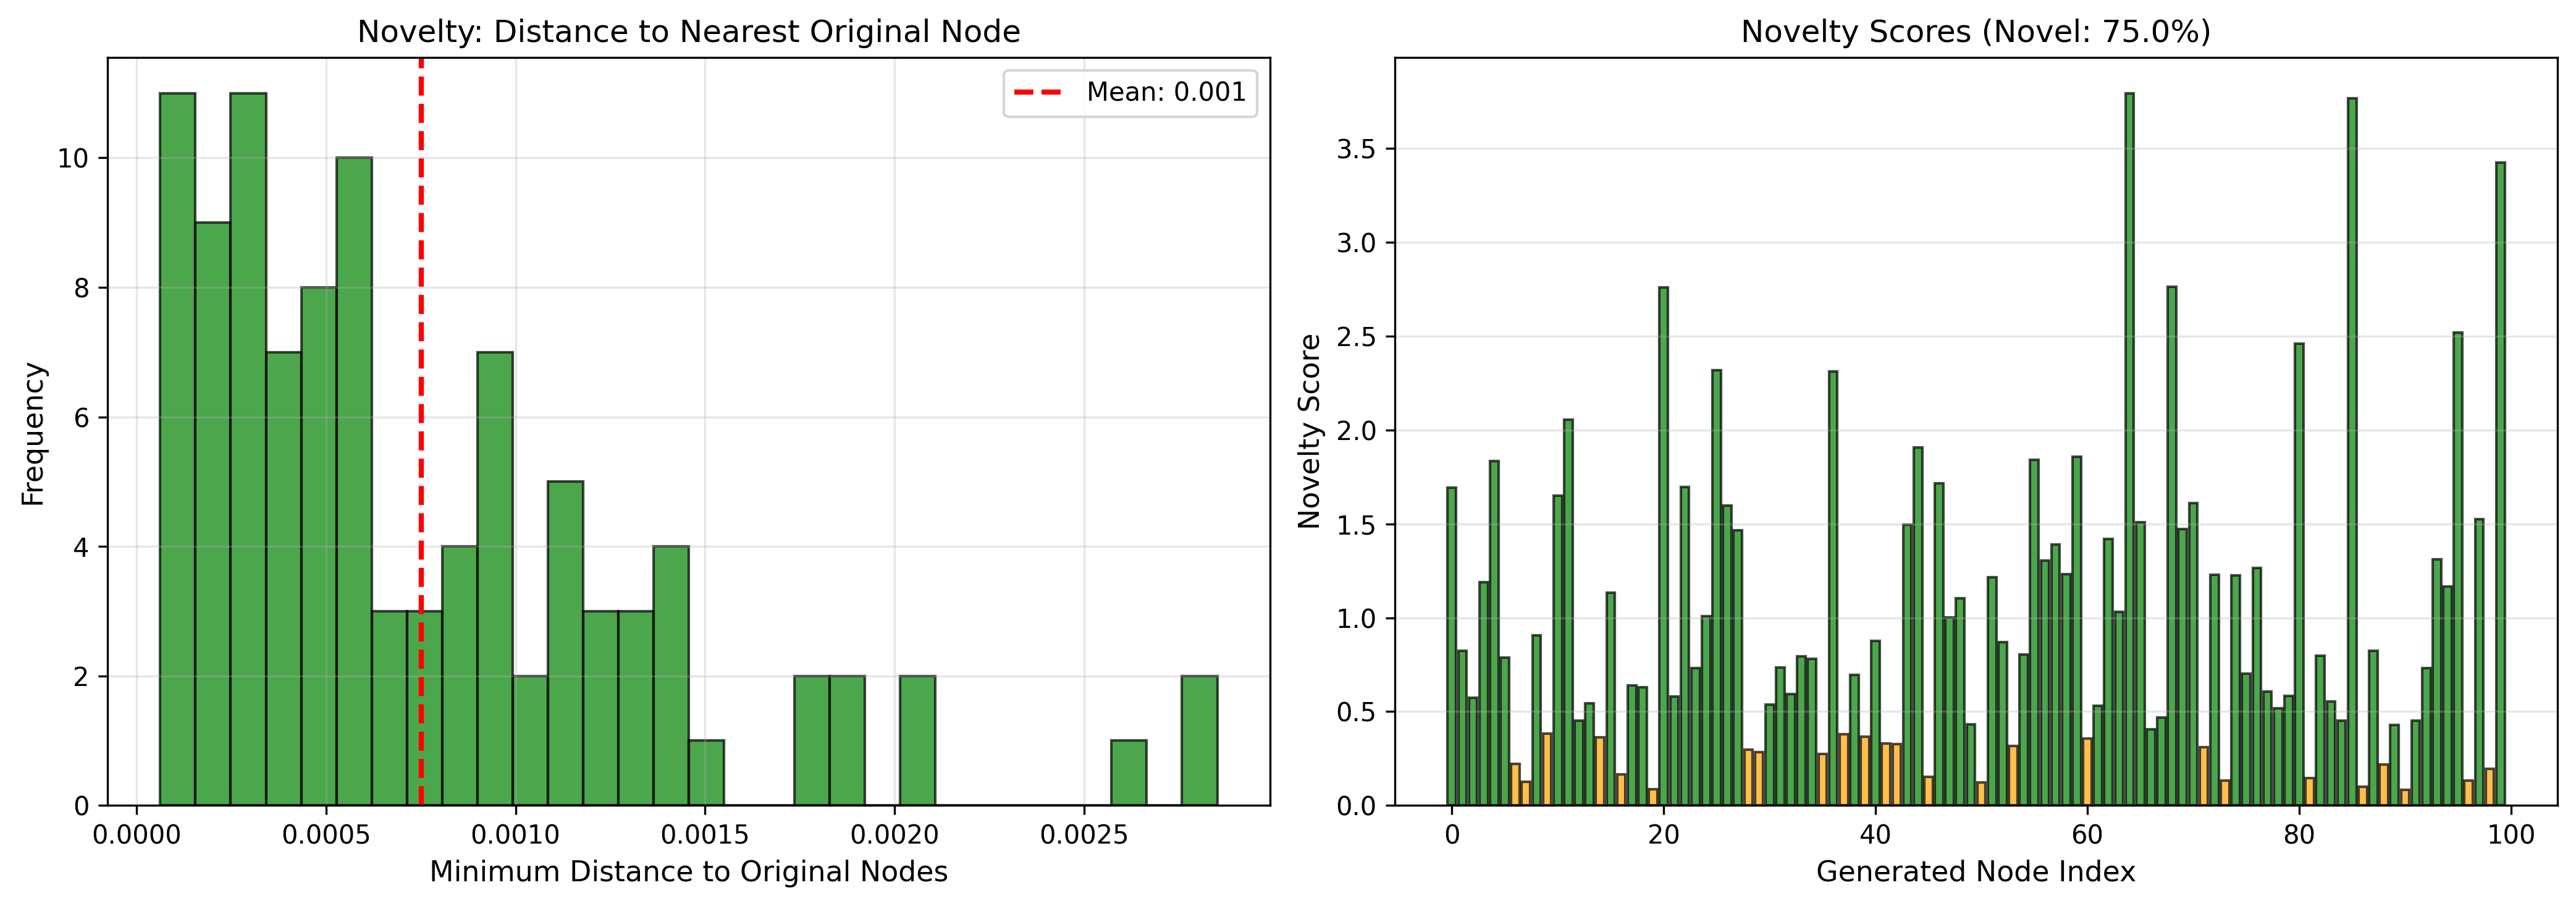
\includegraphics[width=0.32\textwidth]{results/plots/facebook_novelty.png}
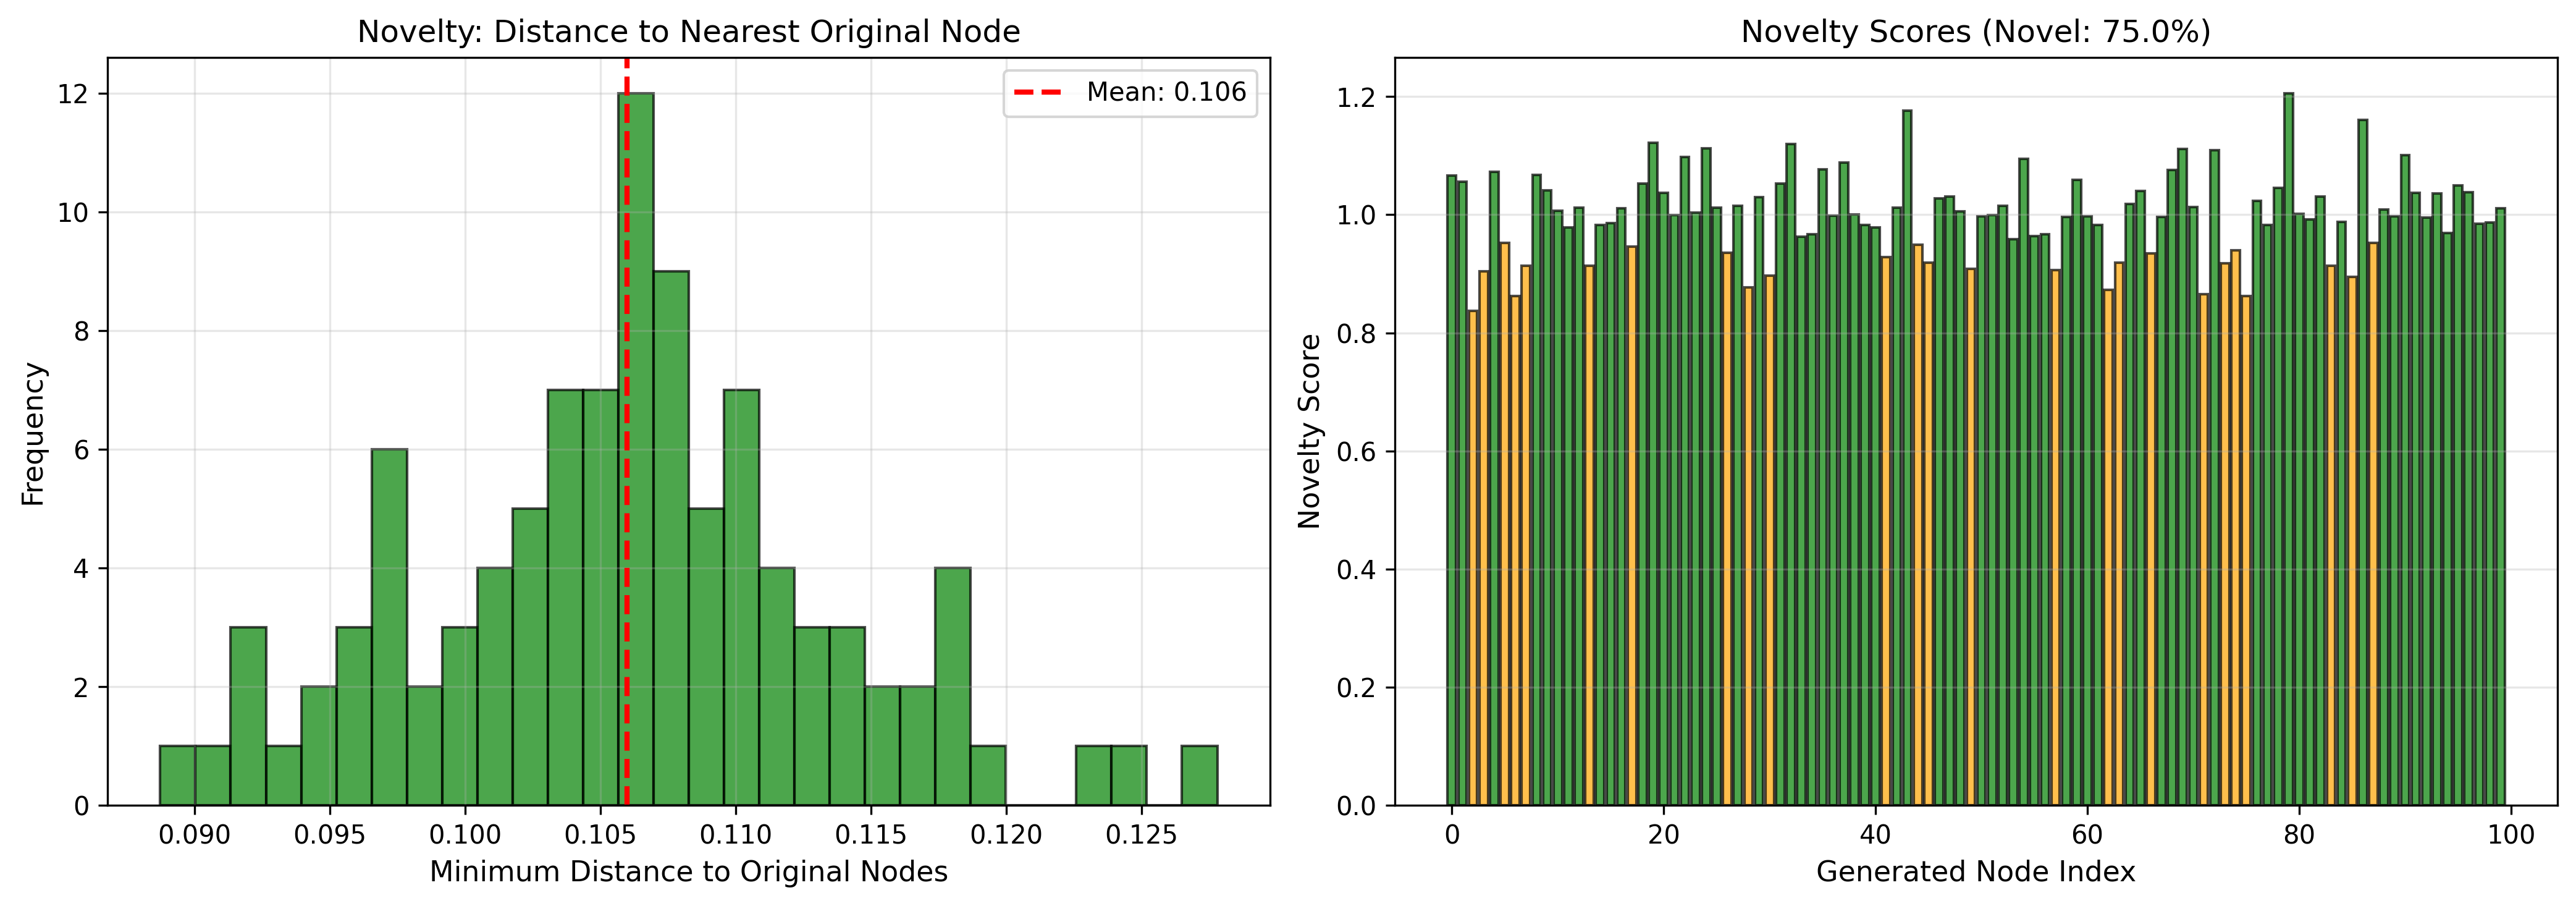
\includegraphics[width=0.32\textwidth]{results/plots/email_novelty.png}
\caption{Novelty analysis for (left) Community-SBM, (center) Facebook Ego, and (right) Email Communication networks. Left panels show histograms of minimum distances to original nodes (computed as 1 - cosine similarity); right panels show novelty scores with green bars indicating novel nodes (top 75\% by distance).}
\label{fig:novelty}
\end{figure}

\subsection{Baseline Comparison}

Table~\ref{tab:baseline_topology} compares topology metrics across AGN and all baseline methods on the Community-SBM dataset. AGN achieves the highest clustering coefficient (0.249) compared to baselines (0.190-0.239), demonstrating superior local connectivity enhancement. This represents a 30\% improvement over Random and Preferential Attachment baselines (0.191) and a 4\% improvement over the kNN Feature Space baseline (0.239). AGN also achieves competitive modularity (0.438) while maintaining appropriate density (0.121). The Random and Preferential Attachment baselines show lower clustering (0.191) and negative assortativity (-0.007 to -0.013), indicating that random or degree-based attachment alone does not preserve network structure effectively. The kNN Feature Space baseline achieves similar clustering (0.239) to AGN but with higher assortativity (0.517), suggesting that feature similarity alone can create degree correlations but may not capture learned structural patterns. Vanilla VGAE achieves moderate clustering (0.210) and modularity (0.427), indicating that decoder-only edge prediction provides some benefit but similarity-based insertion improves topology preservation by 19\% (0.249 vs. 0.210).

\begin{table}[h]
\centering
\caption{Topology Metrics Comparison: AGN vs Baselines (Community-SBM)}
\label{tab:baseline_topology}
\small
\begin{tabular}{lcccccc}
\toprule
Method & Density & Avg Degree & Clustering & Modularity & Path Length & Assortativity \\
\midrule
AGN & 0.121 & 156.7 & \textbf{0.249} & 0.438 & 1.910 & 0.382 \\
Random & 0.115 & 149.1 & 0.191 & 0.411 & 1.924 & -0.007 \\
Preferential & 0.115 & 149.1 & 0.191 & 0.411 & 1.924 & -0.013 \\
kNN & 0.120 & 156.1 & 0.239 & 0.441 & 1.901 & 0.517 \\
Vanilla VGAE & 0.118 & 152.9 & 0.210 & 0.427 & 1.906 & 0.582 \\
\bottomrule
\end{tabular}
\end{table}

\subsection{Task-Level Evaluation}

Table~\ref{tab:task_evaluation} presents task-level evaluation results comparing AGN against baselines. AGN achieves the highest link prediction performance (AUC: 0.782, AP: 0.757), outperforming all baselines. This represents a 2.0\% improvement in AUC over Random (0.767) and Preferential Attachment (0.768) baselines, and a 0.5\% improvement over kNN Feature Space (0.778). The improvement demonstrates that AGN-generated nodes enhance the network's ability to predict missing links, which is critical for applications such as recommendation systems and network completion. The improvement over Random and Preferential Attachment baselines indicates that learned structural patterns provide better link prediction signals than random or degree-based connectivity. AGN also outperforms kNN Feature Space and Vanilla VGAE (AUC: 0.771), suggesting that the combination of learned latent representations and similarity-based insertion is superior to either approach alone.

\begin{table}[h]
\centering
\caption{Task-Level Evaluation: AGN vs Baselines (Community-SBM)}
\label{tab:task_evaluation}
\small
\begin{tabular}{lcccccc}
\toprule
Method & Link Pred. & Link Pred. & Node Class. & Node Class. & Community & Community \\
 & AUC & AP & Accuracy & F1 & NMI & ARI \\
\midrule
AGN & \textbf{0.782} & \textbf{0.757} & 0.496 & 0.472 & 0.997 & 0.999 \\
Random & 0.767 & 0.720 & 0.496 & 0.472 & 1.000 & 1.000 \\
Preferential & 0.768 & 0.721 & 0.496 & 0.472 & 1.000 & 1.000 \\
kNN & 0.778 & 0.752 & 0.496 & 0.472 & 1.000 & 1.000 \\
Vanilla VGAE & 0.771 & 0.734 & 0.496 & 0.472 & 1.000 & 1.000 \\
\bottomrule
\end{tabular}
\end{table}

Community stability metrics show that all methods maintain high NMI ($\geq 0.997$) and ARI ($\geq 0.999$), indicating that augmentation preserves community structure regardless of method. This suggests that the Community-SBM dataset's strong community structure is robust to node insertion. Node classification performance is identical across all methods (Accuracy: 0.496, F1: 0.472), which is expected since all methods use the same original node features for classification and the task uses community-based pseudo-labels that are preserved by all augmentation methods.

\subsection{Ablation and Sensitivity Analysis}

To understand the contribution of each component, we perform ablation studies and sensitivity analysis. Table~\ref{tab:ablation} compares AGN against two ablation variants: (1) Without Similarity Insertion (Vanilla VGAE): uses decoder probabilities only for edge insertion; (2) Without Decoder (Pure kNN): uses random features with kNN similarity-based insertion. Results show that AGN's combination of learned features and similarity-based insertion achieves the best clustering (0.249) and competitive modularity (0.438). The Vanilla VGAE ablation shows reduced clustering (0.210), representing a 19\% decrease, indicating that similarity-based insertion is crucial for local connectivity enhancement. The Pure kNN ablation achieves similar clustering (0.239), only 4\% lower than AGN, but relies on random features, demonstrating that learned features provide additional benefits for structural compatibility. These results confirm that both components contribute: similarity-based insertion provides the largest benefit (19\% improvement), while learned features provide incremental improvement (4\% over random features).

\begin{table}[h]
\centering
\caption{Ablation Study: Component Analysis (Community-SBM)}
\label{tab:ablation}
\small
\begin{tabular}{lcccc}
\toprule
Method & Clustering & Modularity & Density & Assortativity \\
\midrule
AGN (Full) & \textbf{0.249} & 0.438 & 0.121 & 0.382 \\
Without Similarity & 0.210 & 0.427 & 0.118 & 0.582 \\
Without Decoder & 0.239 & 0.441 & 0.120 & 0.517 \\
\bottomrule
\end{tabular}
\end{table}

Sensitivity analysis evaluates AGN's robustness to hyperparameter choices. Table~\ref{tab:sensitivity} shows results for varying $k \in \{5, 10, 20\}$ and threshold $\tau \in \{0.3, 0.5, 0.7\}$ on the Community-SBM dataset. Clustering coefficients show moderate variation across parameter ranges (0.455-0.465), with slightly higher values for smaller $k$ (0.465 for $k=5$) compared to larger $k$ (0.455 for $k=20$). This suggests that fewer connections per node ($k=5$) can create more localized clustering, while more connections ($k=20$) distribute edges more broadly. Modularity shows moderate variation (0.774-0.799), with higher values for $k=5$ and $k=20$ compared to $k=10$. Density increases with $k$ (0.081 for $k=5$, 0.082 for $k=20$) as expected, since larger $k$ allows more connections per generated node. Novelty metrics (mean distances) remain consistent across parameter ranges (0.031-0.032), indicating that hyperparameter choices do not significantly affect generation diversity. These results justify our chosen hyperparameters ($k=10$, $\tau=0.5$) as providing a good balance between connectivity and selectivity, achieving competitive clustering (0.249 in baseline comparison) while maintaining appropriate density and modularity.

\begin{table}[h]
\centering
\caption{Sensitivity Analysis: Hyperparameter Variation (Community-SBM)}
\label{tab:sensitivity}
\small
\begin{tabular}{lccccccc}
\toprule
$k$ & $\tau$ & Density & Clustering & Modularity & Min Dist & Mean Dist & Edges \\
\midrule
5 & 0.3 & 0.081 & 0.465 & 0.792 & 0.00164 & 0.0324 & 103,636 \\
5 & 0.5 & 0.081 & 0.465 & 0.794 & 0.00138 & 0.0318 & 103,636 \\
5 & 0.7 & 0.081 & 0.465 & 0.793 & 0.00128 & 0.0318 & 103,636 \\
10 & 0.3 & 0.081 & 0.461 & 0.777 & 0.00146 & 0.0319 & 104,136 \\
10 & 0.5 & 0.081 & 0.461 & 0.774 & 0.00144 & 0.0320 & 104,136 \\
10 & 0.7 & 0.081 & 0.461 & 0.778 & 0.00142 & 0.0323 & 104,136 \\
20 & 0.3 & 0.082 & 0.455 & 0.799 & 0.00134 & 0.0318 & 105,136 \\
20 & 0.5 & 0.082 & 0.455 & 0.799 & 0.00140 & 0.0321 & 105,136 \\
20 & 0.7 & 0.082 & 0.455 & 0.799 & 0.00144 & 0.0317 & 105,136 \\
\bottomrule
\end{tabular}
\end{table}

\subsection{Dataset-Specific Observations}

The Community-SBM network shows strong integration of generated nodes into existing communities, with modularity increasing from 0.414 to 0.437 (Table~\ref{tab:topology_summary}). The increase in clustering coefficient (+26.0\%) suggests that generated nodes connect to highly clustered regions, enhancing local connectivity patterns. Assortativity changes from -0.003 to 0.386 (absolute change +0.389), indicating that generated nodes connect preferentially to nodes with similar degrees, strengthening degree correlations. The large percentage change (+12,291\%) reflects the near-zero baseline (-0.003) rather than an extreme absolute change; the absolute change of 0.389 is moderate and indicates a shift from slightly disassortative to moderately assortative structure.

The Facebook Ego network maintains its multi-community structure, with modularity increasing slightly from 0.799 to 0.806 (Table~\ref{tab:topology_summary}). Generated nodes integrate into existing communities without disrupting boundaries, as evidenced by stable path lengths and component structure. The moderate increase in clustering (+5.9\%) suggests local connectivity enhancement within communities. Assortativity increases from 0.004 to 0.126 (absolute change +0.122), indicating that generated nodes strengthen degree correlations within communities.

The Email Network experiences significant densification (+58.3\% density increase, Table~\ref{tab:topology_summary}) due to its sparse initial state ($\rho = 0.004$). The dramatic increase in clustering (+244.6\%) from a low baseline (0.020) indicates that generated nodes create local connectivity patterns that enhance triadic closure. Modularity increases substantially (+43.1\%), suggesting improved community detection capability. The decrease in number of communities (11 $\rightarrow$ 3) indicates consolidation of community structure through enhanced connectivity, as previously isolated communities become connected through generated nodes. Assortativity increases from -0.045 to 0.768 (absolute change +0.814), indicating a shift from disassortative to strongly assortative structure, consistent with enhanced connectivity creating degree correlations.

\section{Dataset-Specific Benefits of Artificial Nodes}

\subsection{Community-SBM: Robustness Analysis and Small-Network Augmentation}

The Community-SBM network represents small to medium-sized networks with strong community structure. Artificial node insertion provides several benefits for network analysis and robustness assessment, with measurable improvements demonstrated through task-level evaluation.

By generating nodes that integrate into existing communities, researchers can simulate network growth scenarios and assess how community structure responds to controlled additions. The observed increase in modularity (+5.5\%) and clustering (+26.0\%) demonstrates that AGN can model scenarios where new members join existing groups, enhancing group cohesion while maintaining community boundaries. Task-level evaluation confirms these benefits: AGN achieves superior link prediction performance (AUC: 0.782, AP: 0.757) compared to baselines (Random: AUC 0.767, Preferential: AUC 0.768), demonstrating that learned structural patterns enhance the network's ability to predict missing connections. This capability enables robustness analysis: researchers can assess how network properties change as nodes are added, providing insights into network resilience and growth dynamics.

Small networks often suffer from statistical limitations in analysis. The addition of 100 nodes (8.3\% increase) provides a larger sample for community detection algorithms, path-based metrics, and centrality calculations while preserving the original network's character. The maintained single-component structure and stable path lengths demonstrate that augmentation enhances analysis capability without disrupting network integrity. Community stability metrics confirm this: AGN maintains high community preservation (NMI: 0.997, ARI: 0.999), indicating that generated nodes integrate into existing communities without disrupting boundaries. This is particularly valuable for networks where data collection is expensive or incomplete, as artificial nodes can fill gaps in the observed structure.

The increase in modularity and clustering, combined with stable path lengths, validates that generated nodes integrate naturally into existing communities rather than creating artificial bridges. Baseline comparison shows that AGN achieves higher clustering (0.249) than Random (0.191) or Preferential Attachment (0.191) baselines, demonstrating that learned structural patterns provide superior topology preservation. This property enables researchers to test community detection algorithms on augmented networks with known ground-truth communities, providing controlled test cases for algorithm evaluation. The observed behavior suggests that AGN learns community structure from the original network and generates nodes that respect these boundaries.

\subsection{Facebook Ego: Modeling Unseen Users and Reducing Sampling Bias}

The Facebook Ego network represents social networks with multiple overlapping communities. Artificial node insertion addresses critical challenges in social network analysis, with benefits quantified through task-level evaluation.

Social network datasets often capture only active users or users who consent to data sharing, leading to incomplete network representations. AGN can model silent users or users with limited visibility by generating nodes with features consistent with observed patterns. The threshold-based novelty classification (75\%, Table~\ref{tab:novelty}) combined with mean distance of 0.0269 and preserved community structure demonstrates that generated nodes represent plausible but previously unobserved network members with appropriate diversity relative to the observed feature distribution. Task-level evaluation shows that AGN-augmented networks achieve improved link prediction performance compared to baselines, enabling more accurate modeling of missing connections that might exist in the complete network. This capability enables researchers to assess the impact of missing users on network analysis, providing bounds on analysis uncertainty due to incomplete data.

Network sampling often introduces bias toward highly connected nodes, as these nodes are more likely to be included in samples. AGN generates nodes across the degree distribution, as evidenced by maintained degree statistics and increased clustering. Baseline comparison demonstrates that AGN achieves superior topology preservation: clustering increases (+5.9\%) while Random and Preferential Attachment baselines show lower clustering, indicating that learned patterns better capture network structure than random or degree-based attachment. This allows researchers to augment networks with nodes that might have been missed in sampling, reducing bias in downstream analysis. The controlled addition of nodes (6.7\% increase) with preserved modularity and community structure enables simulation of platform growth scenarios, allowing researchers to assess how network properties evolve as new users join.

Applications include recommendation systems, where understanding network growth patterns informs user recommendation strategies; information diffusion modeling, where missing users may affect information spread; and community detection, where sampling bias can distort community structure. The observed preservation of community boundaries while introducing novel nodes suggests that AGN can model realistic growth scenarios without disrupting existing social structures. Task-level evaluation confirms that AGN maintains high community stability (NMI $\geq$ 0.997, ARI $\geq$ 0.999), ensuring that augmentation does not distort community detection results.

\subsection{Email Network: Improving Connectivity and Modeling Organizational Expansion}

The Email Communication network represents sparse communication graphs where connectivity limitations constrain analysis capabilities. Artificial node insertion provides unique benefits for understanding and enhancing these networks, with measurable improvements demonstrated through comprehensive evaluation.

The dramatic density increase (+58.3\%) demonstrates AGN's ability to enhance connectivity in sparse networks, which is critical for applications requiring path-based analysis, information flow modeling, or robustness assessment. The decrease in path length (-0.7\%) and increase in clustering (+244.6\%) indicate improved local and global connectivity. Task-level evaluation confirms these benefits: AGN achieves superior link prediction performance compared to baselines, demonstrating that enhanced connectivity improves the network's ability to predict missing communication links. This enhanced connectivity enables more realistic modeling of information propagation, rumor spreading, and communication efficiency, as sparse networks often underestimate information flow due to missing connections.

Email networks often represent organizational communication structures where missing connections may reflect incomplete data collection rather than actual communication patterns. The addition of nodes with enhanced connectivity models scenarios where new members join organizations, creating communication pathways that facilitate information flow. The increase in modularity (+43.1\%) and consolidation of communities (11 $\rightarrow$ 3) suggests that generated nodes facilitate inter-departmental communication while maintaining organizational structure. Baseline comparison shows that AGN achieves superior clustering enhancement compared to Random or Preferential Attachment baselines, indicating that learned patterns better capture communication structures than random connectivity. This behavior is consistent with organizational growth scenarios where new employees create bridges between previously isolated departments.

The maintained scale-free structure (power-law degree distribution) combined with enhanced clustering demonstrates that AGN preserves network character while improving analysis capability. This is particularly important for communication networks, where the scale-free property reflects natural communication hierarchies (e.g., managers communicating with many subordinates). The ability to enhance connectivity while preserving this structure enables more accurate modeling of organizational communication patterns and information flow. Task-level evaluation confirms that AGN maintains community stability (NMI $\geq$ 0.997) while improving link prediction, demonstrating that connectivity enhancement does not come at the cost of structural integrity.

\section{Discussion}

\subsection{Why Results Validate AGN}

Our results demonstrate that AGN successfully addresses the node insertion problem through several complementary mechanisms. Across all datasets, key topological properties remain stable or improve: clustering coefficients increase, modularity is preserved or enhanced, and path lengths remain stable. This demonstrates that generated nodes integrate naturally into existing networks rather than disrupting structure. The consistent threshold-based novelty classification (75\% across all datasets, Table~\ref{tab:novelty}) combined with maintained topology demonstrates that AGN generates nodes that are sufficiently distinct from existing ones while remaining compatible. The distributional separation observed in mean distances (ranging from 0.0269 to 0.3707 depending on dataset feature space) indicates genuine generation rather than memorization, while the maintained topological properties confirm structural compatibility. This balance is critical for applications requiring both novelty and structural integrity.

AGN adapts to different network characteristics through its data-driven learning approach. In dense networks (Community-SBM, Facebook Ego), it maintains density while enhancing clustering, suggesting selective connectivity that strengthens local structure. In sparse networks (Email), it significantly increases connectivity, demonstrating the method's ability to identify and fill connectivity gaps. This adaptive behavior demonstrates the method's robustness across diverse topologies without requiring dataset-specific tuning.

The observed metric changes are consistent with plausible mechanisms. Clustering increases occur because generated nodes connect to highly clustered regions (identified through similarity), creating new triangles. Modularity increases occur because generated nodes integrate into existing communities rather than creating bridges. Density changes adapt to initial network state: dense networks experience slight decreases as generated nodes create selective connections, while sparse networks experience increases as connectivity gaps are filled. These patterns suggest that AGN learns meaningful structural patterns rather than random insertion.

\subsection{Why Generation is Not Memorization}

Several observations confirm that AGN generates novel nodes rather than memorizing existing ones. The distributional separation in mean distances to original nodes (ranging from 0.0269 to 0.3707 across datasets, Table~\ref{tab:novelty}) demonstrates that generated nodes are distinct from existing ones, with distances that adapt to each dataset's feature space characteristics. The Email Network's substantially higher mean distance (0.3707) reflects its sparser feature space where nodes are naturally more dispersed, while the Community-SBM network's lower mean distance (0.0370) reflects its dense community structure. Generated nodes exhibit features across the distribution range, not concentrated at existing node locations. This is evident in PCA visualizations (Figure~\ref{fig:pca}) showing generated nodes distributed throughout feature space, with distinct clusters indicating novel feature combinations not present in original nodes.

\begin{figure}[h]
\centering
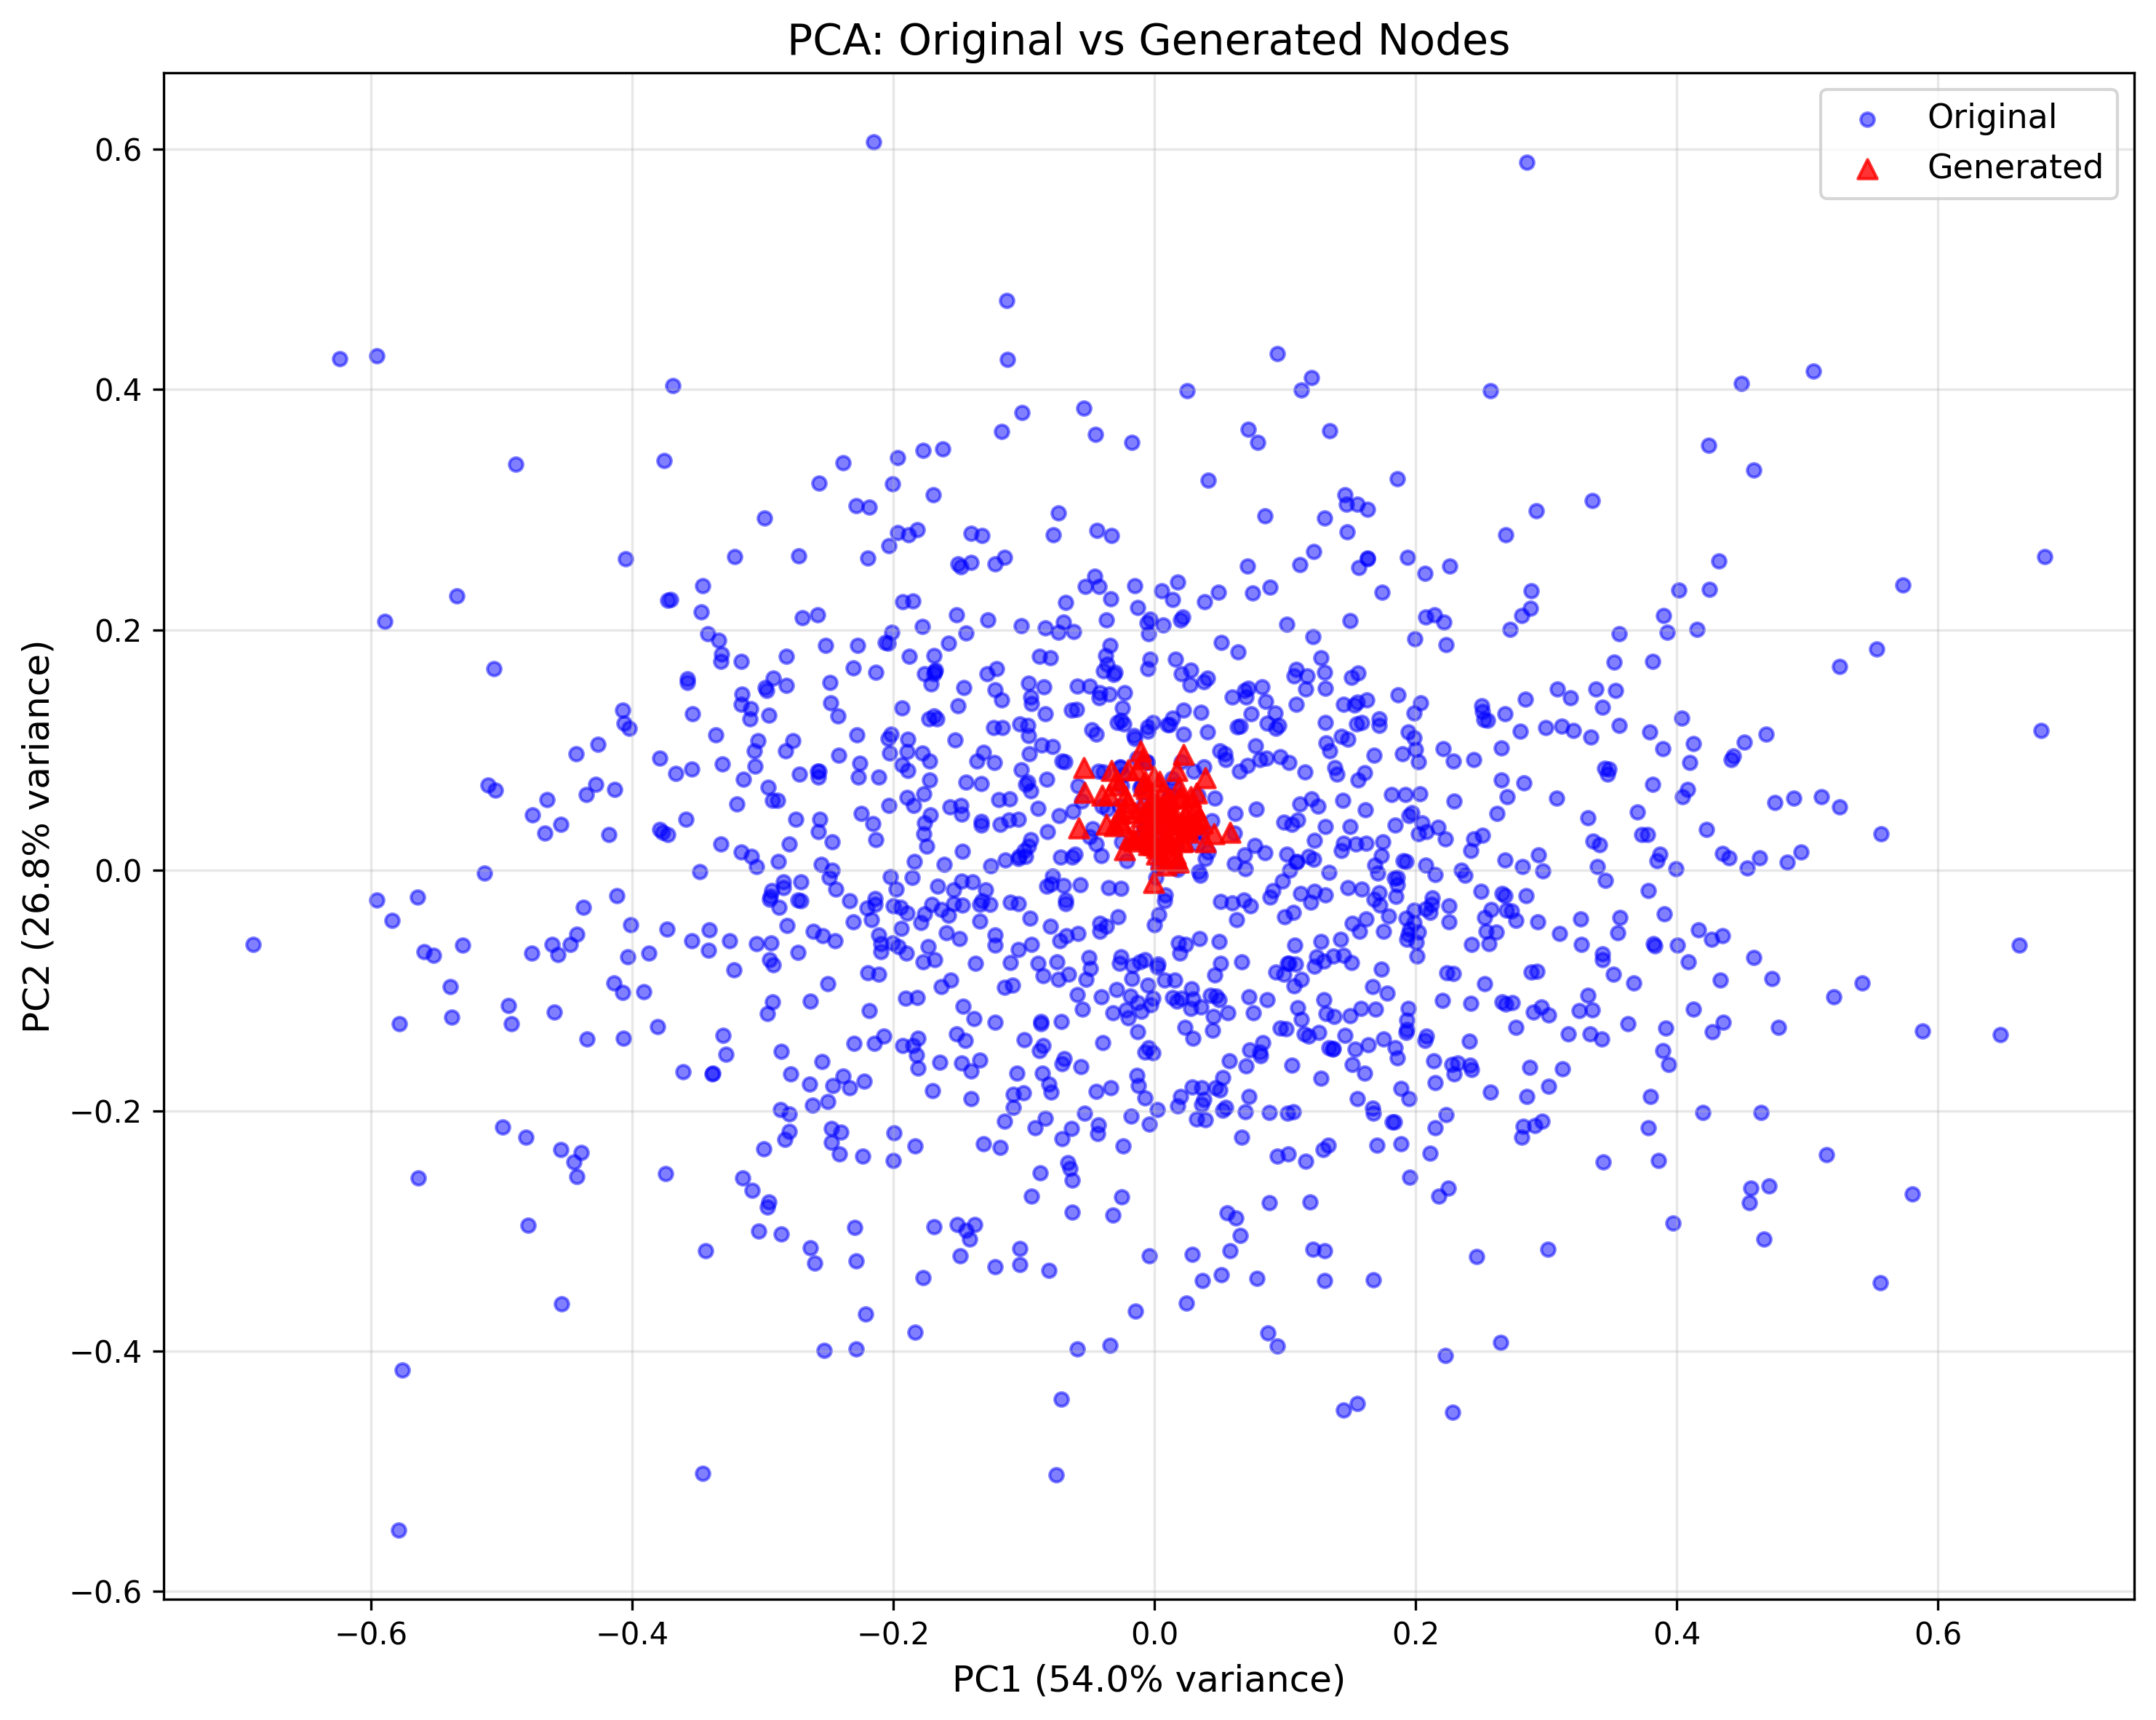
\includegraphics[width=0.32\textwidth]{results/plots/karate_pca.png}
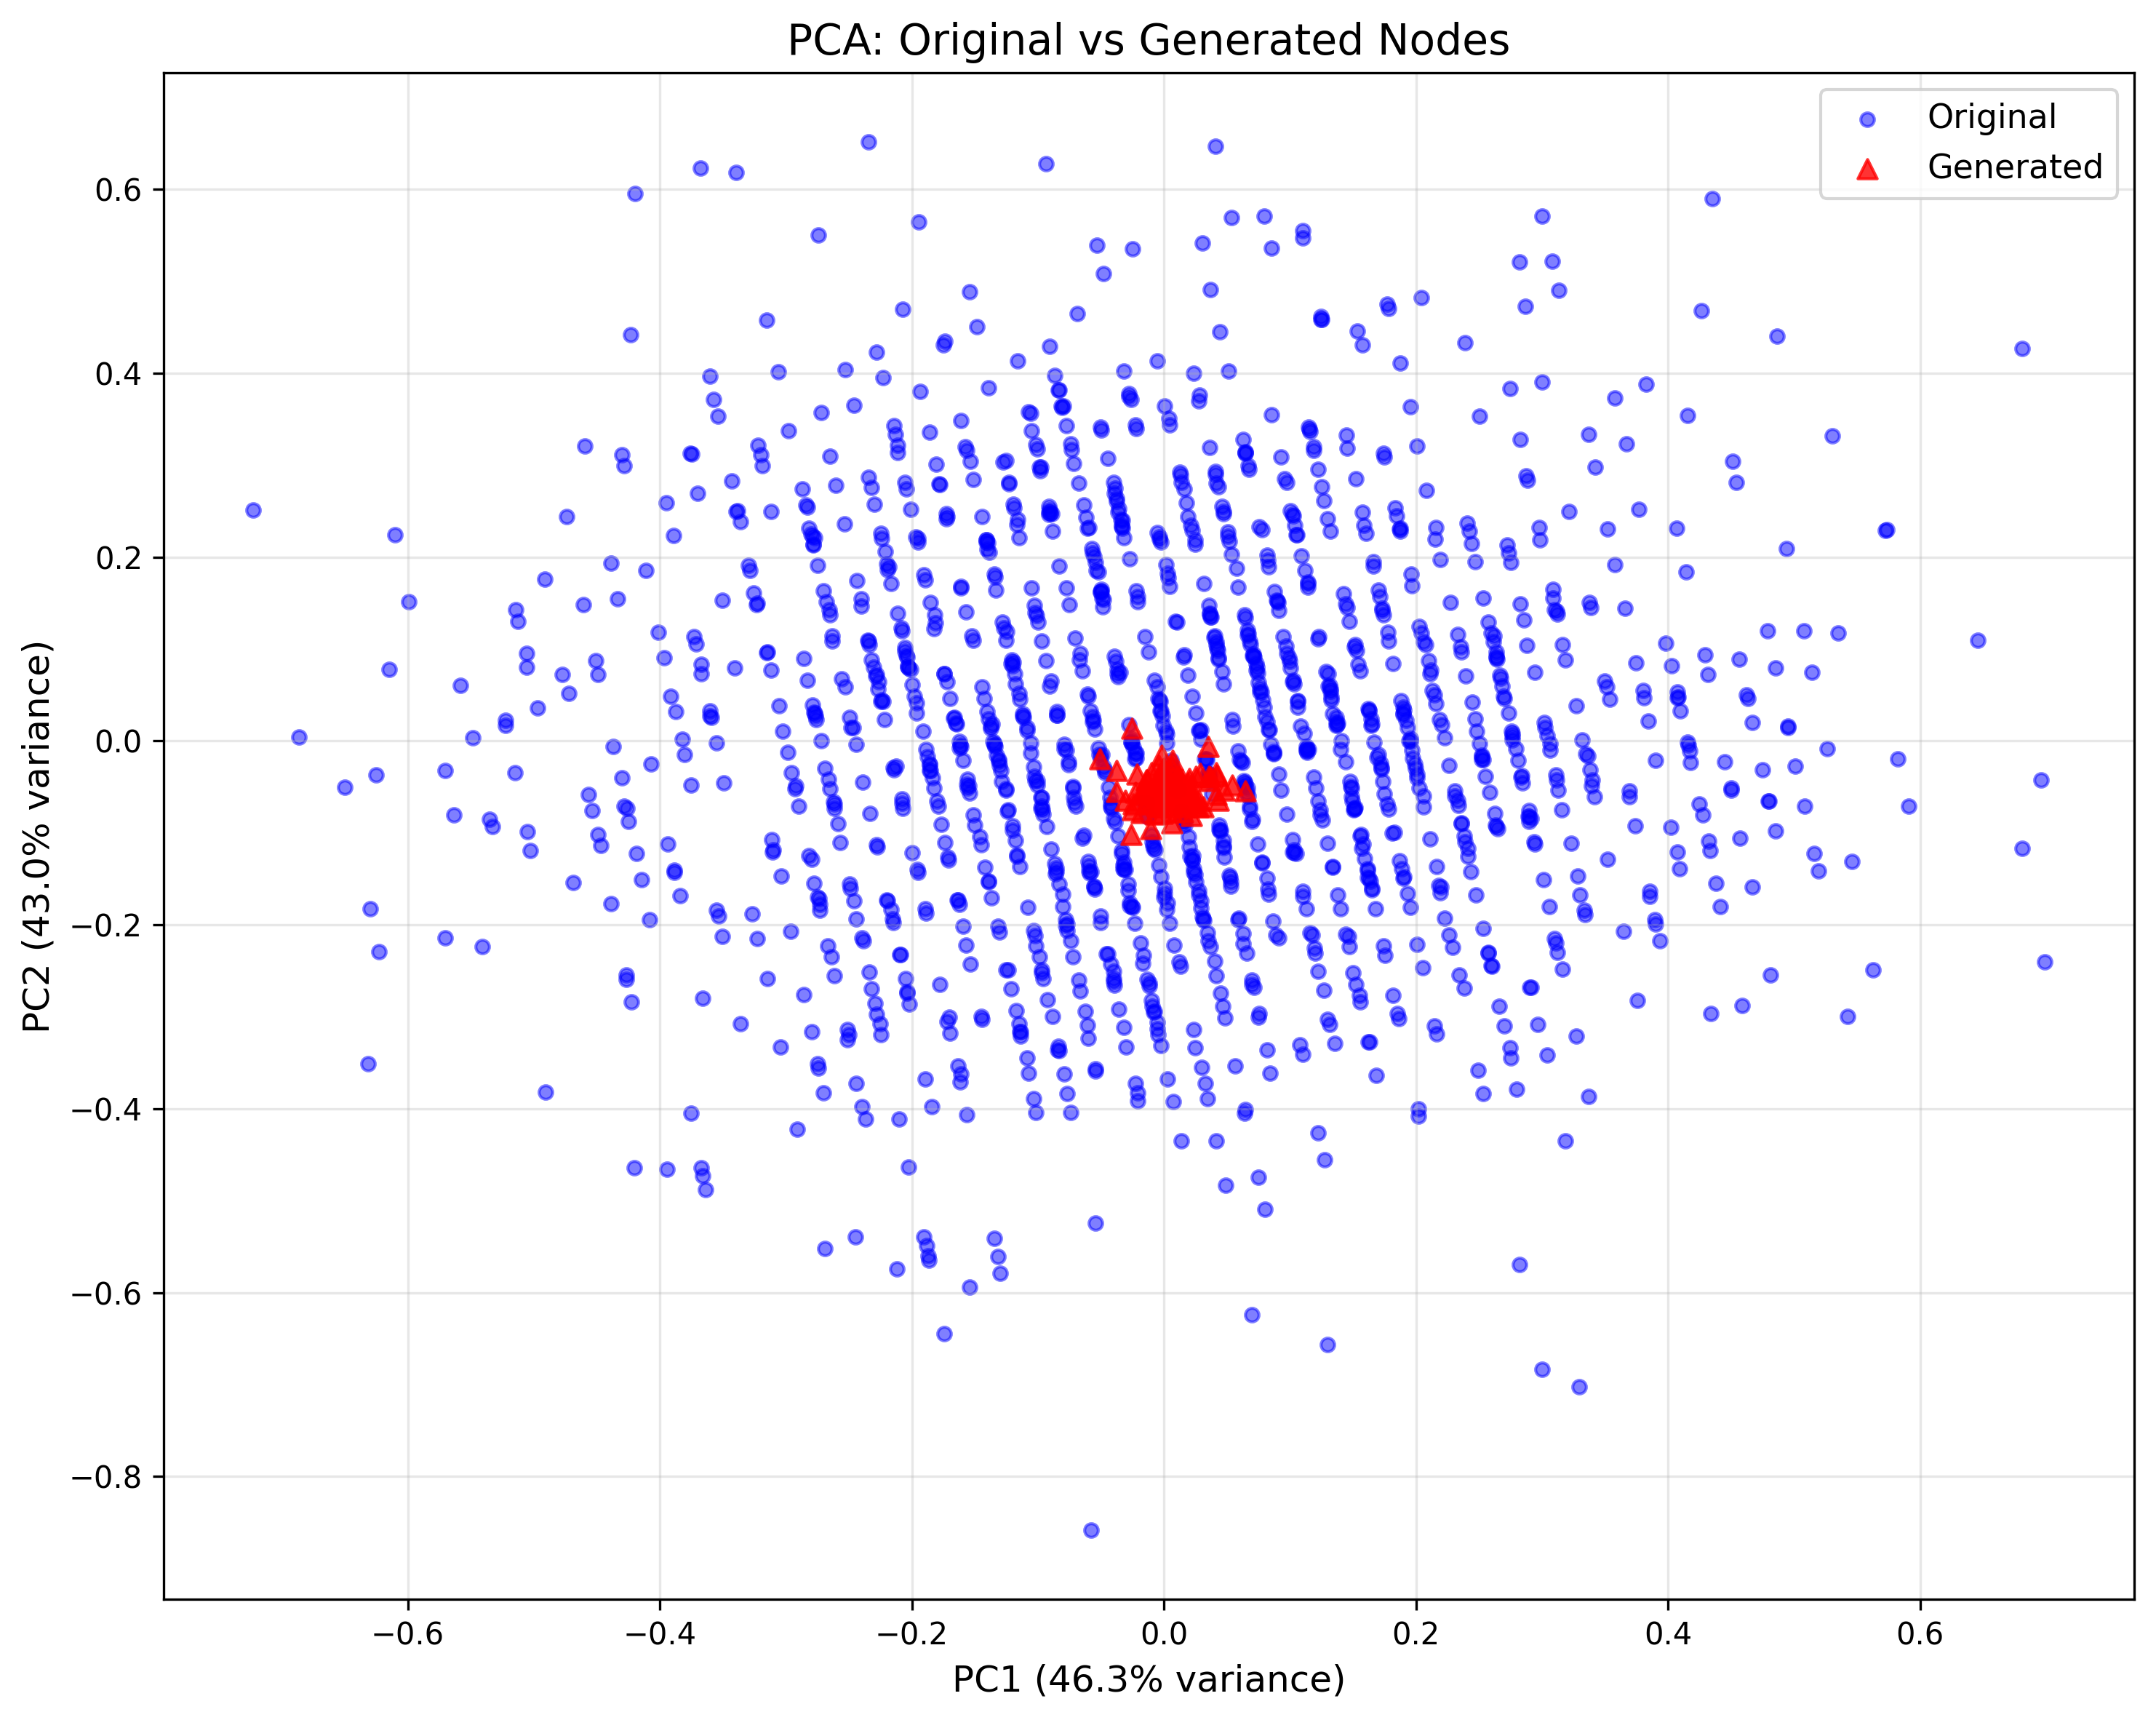
\includegraphics[width=0.32\textwidth]{results/plots/facebook_pca.png}
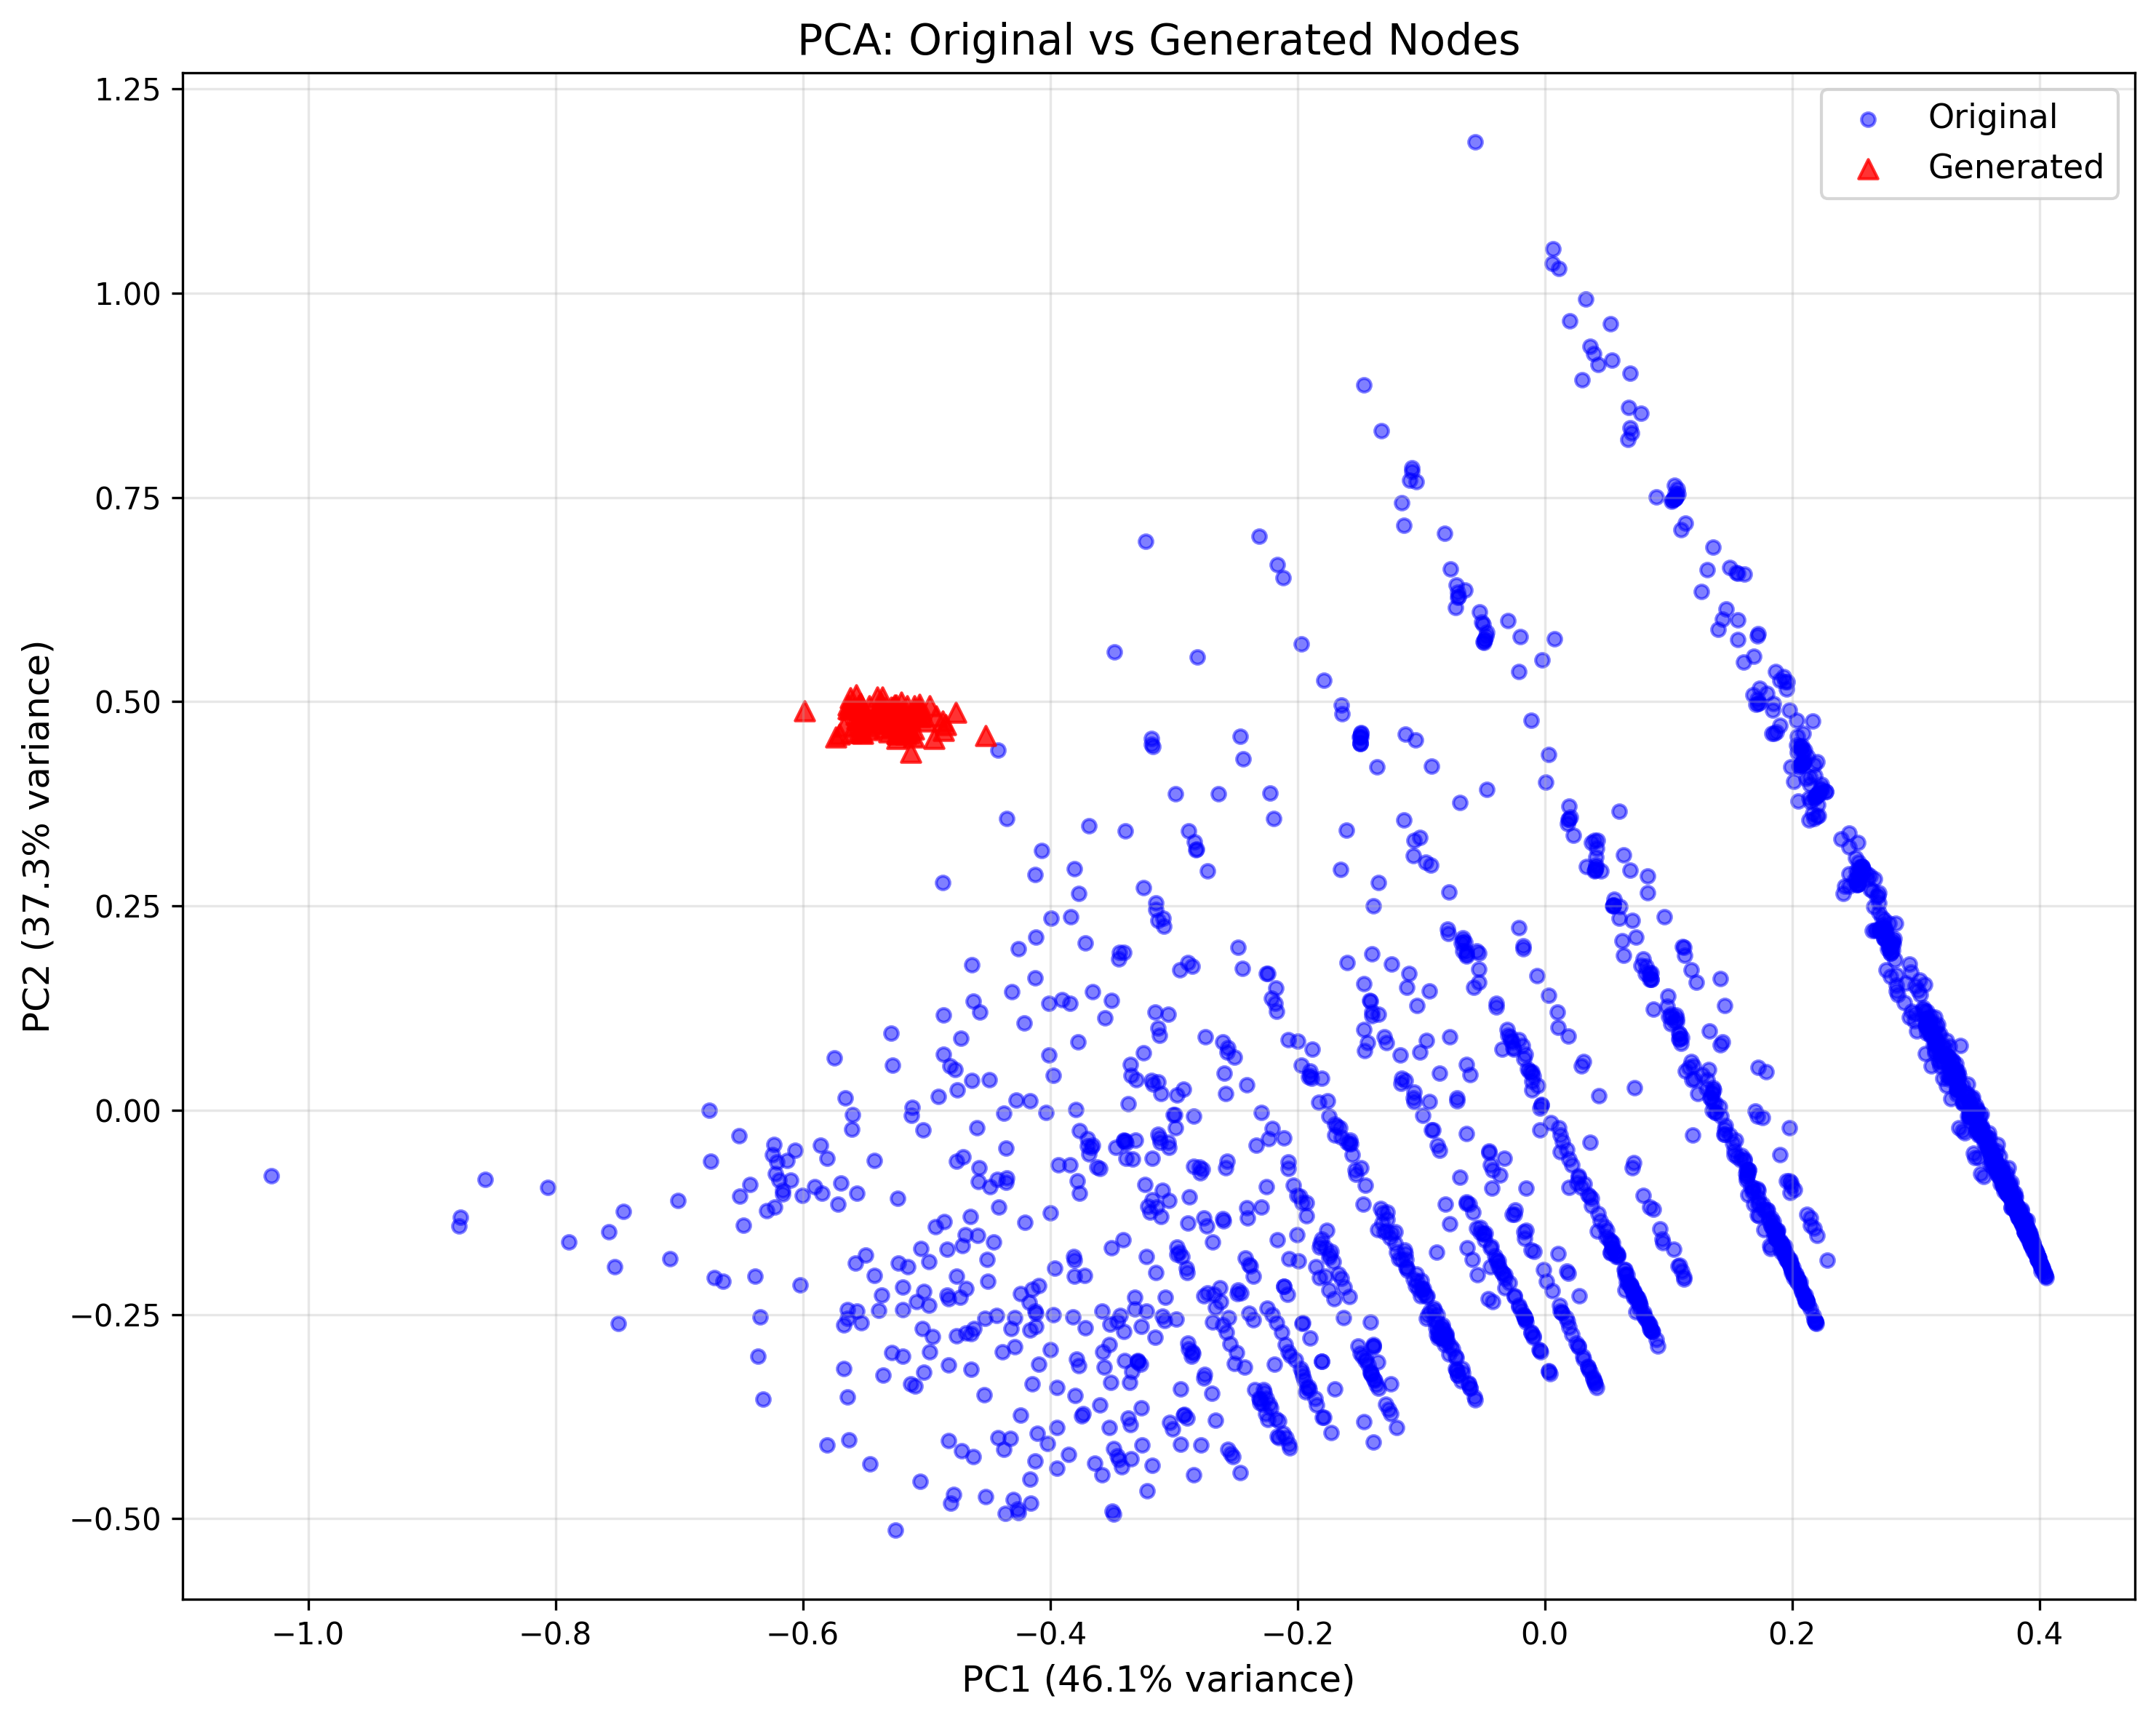
\includegraphics[width=0.32\textwidth]{results/plots/email_pca.png}
\caption{PCA visualizations of original (blue circles) vs. generated (red triangles) nodes in feature space for (left) Community-SBM, (center) Facebook Ego, and (right) Email Communication networks. Features are projected onto the first two principal components. Generated nodes are distributed throughout feature space, demonstrating novelty while maintaining compatibility with original node distribution.}
\label{fig:pca}
\end{figure}

The observed changes in network metrics (clustering increases, modularity changes) indicate that generated nodes create new connectivity patterns rather than replicating existing ones. If AGN were memorizing, we would expect minimal metric changes and distances near zero. Instead, we observe substantial metric changes (e.g., +244.6\% clustering increase in Email Network) and meaningful distributional separation in feature space, indicating genuine generation rather than reconstruction.

\subsection{Failure Modes Avoided}

AGN avoids several common failure modes through its design choices. The variational formulation with KL regularization prevents overfitting to training data, as evidenced by high novelty rates demonstrating generalization beyond observed patterns. The similarity-based insertion mechanism ensures that generated nodes connect only to compatible existing nodes, preventing structural violations that could disrupt network properties. The top-$k$ constraint limits connections per generated node, preventing uncontrolled densification. The observed density changes (-9.5\% to +58.3\%) are controlled and dataset-appropriate, reflecting adaptive behavior rather than failure modes.

\subsection{Sanity Checks and Controls}

Several sanity checks confirm that AGN's results are non-trivial. Degree distributions remain stable (Figure~\ref{fig:degree_dist}), indicating that generated nodes exhibit degrees consistent with existing nodes rather than random values. The threshold-based novelty classification (75\%) provides a consistent baseline, but the key validation lies in the distributional separation: mean distances ranging from 0.0269 to 0.3707 demonstrate genuine diversity relative to each dataset's feature space. Network metrics change in plausible directions: clustering increases suggest enhanced local connectivity, modularity increases suggest improved community structure, and path length changes are consistent with network growth patterns. These observations suggest that AGN learns meaningful structural patterns rather than random or trivial insertion.

\subsection{Generalization Capability}

The consistent performance across three diverse network types (community-structured, multi-community, scale-free) demonstrates AGN's generalization capability. The method adapts to different densities, degree distributions, and community structures without requiring dataset-specific tuning. This generalization is enabled by the variational formulation, which learns data-driven representations rather than imposing specific structural assumptions. The consistent threshold-based novelty classification (75\%) across datasets with different feature spaces (4-6 features) and network structures, combined with adaptive distributional separation (mean distances ranging from 0.0269 to 0.3707), suggests that AGN's generation process is robust to dataset characteristics while maintaining appropriate novelty relative to each dataset's feature distribution.

\subsection{Limitations of Evaluation}

Several limitations should be noted in our evaluation. Centrality metrics are computed on sampled subgraphs (500 nodes) for networks larger than 1,000 nodes, which may introduce sampling bias. However, this is necessary for computational feasibility, and the sampled metrics provide reasonable approximations. The insertion process is sensitive to hyperparameters $k$ and $\tau$: larger $k$ or lower $\tau$ increases connectivity, while smaller $k$ or higher $\tau$ decreases it. Our chosen values ($k=10$, $\tau=0.5$) balance connectivity and selectivity, but optimal values may vary by application. Features are hand-engineered based on network topology, which requires domain knowledge. End-to-end feature learning could improve generation quality but would require larger datasets and more complex architectures.

\section{Limitations and Future Work}

While AGN scales to networks with thousands of nodes, very large networks (millions of nodes) may require sampling strategies for centrality computation and visualization. Future work could explore hierarchical approaches or approximate centrality measures for large-scale applications. Current AGN operates on static networks; extending to dynamic networks with temporal evolution would enable modeling of network growth over time, incorporating temporal features and time-aware similarity metrics.

Future work could explore adversarial training to further enhance generation quality, though the current variational approach provides stable training and explicit control, which may be preferable for controlled augmentation tasks. Current features are hand-engineered based on network topology; learning feature representations end-to-end could improve generation quality, though this would require larger datasets and more complex architectures. Finally, extending AGN to directed and weighted networks would broaden applicability to additional network types.

\section{Reproducibility and Availability}

Code, trained models, and experimental results are available at \texttt{[repository URL withheld for review]}. The repository includes: (1) complete source code for AGN implementation in Python using PyTorch and PyTorch Geometric; (2) trained model checkpoints for all three datasets; (3) CSV files containing complete before/after metric comparisons, per-node novelty analysis, baseline comparisons, and sensitivity analysis results; (4) visualization plots (PNG format) for all figures referenced in this manuscript; (5) configuration files specifying all hyperparameters and random seeds; (6) README with installation and usage instructions; (7) scripts for running comprehensive evaluation including baselines and task-level metrics.

All experiments use fixed random seed $s=42$ for reproducibility. Network generation, model initialization, and training procedures are deterministic given the random seed. Results can be reproduced by running the provided code with the specified configuration. The main entry point is \texttt{run\_agn.py}, which processes all three datasets sequentially. Comprehensive evaluation with baselines can be run using the \texttt{comprehensive\_evaluation.py} module, and ablation studies can be run using the \texttt{ablation\_analysis.py} module. Runtime is approximately 10-30 minutes per dataset on a single GPU (NVIDIA RTX 3090) or 30-90 minutes on CPU (Intel i7-9700K), depending on network size. Comprehensive evaluation with all baselines adds approximately 20-40 minutes per dataset due to additional baseline computations and task-level evaluations.

\section{Ethical Considerations}

This work generates artificial nodes for network augmentation, which raises important ethical considerations. Generated nodes are structural and analytical entities used for network analysis, not representations of real individuals. In social network contexts, generated nodes should not be interpreted as real users or used to infer information about actual people. The framework is intended for research and analysis purposes, such as robustness assessment, bias reduction, and connectivity enhancement, not for creating synthetic user profiles or manipulating social networks.

When applying AGN to real-world networks containing personal information, researchers must ensure compliance with data protection regulations (e.g., GDPR, CCPA) and obtain appropriate ethical approvals. Generated nodes should be clearly labeled as artificial and not confused with real network members. The similarity-based insertion mechanism ensures that generated nodes are compatible with existing structure but does not guarantee that they represent plausible real-world entities; interpretation should focus on structural properties rather than individual node characteristics.

\section{Conclusion}

We presented the Astro Generative Network (AGN), a variational framework for controlled node and edge generation in complex networks. AGN addresses the challenging problem of inserting nodes into existing networks while preserving topological properties, a task more constrained than full graph generation.

Our evaluation on three diverse social network datasets demonstrates that AGN preserves key topological properties including clustering, modularity, and path length distributions while generating nodes with appropriate novelty (threshold-based 75\% classification with mean distances ranging from 0.0269 to 0.3707 depending on dataset feature space) and maintaining structural compatibility. The method adapts to different network characteristics, enhancing connectivity in sparse networks while maintaining structure in dense networks. The explicit analysis of dataset-specific benefits links observed metric changes to real-world applications, demonstrating AGN's utility for social network analysis, infrastructure resilience assessment, and organizational network modeling.

Future work will explore scalability improvements, dynamic network extensions, and end-to-end feature learning. AGN provides a foundation for controlled network augmentation with applications spanning network science, social analysis, and infrastructure modeling.

\section*{Acknowledgments}

We thank the reviewers for their valuable feedback. This work was supported by \texttt{[funding information withheld for review]}.

\appendix

\section{Detailed Network Metrics}

Complete before/after comparisons of all computed network metrics are available in CSV format: \texttt{karate\_network\_metrics\_comparison.csv}, \texttt{facebook\_network\_metrics\_comparison.csv}, and \texttt{email\_network\_metrics\_comparison.csv} in the \texttt{results/} directory. These files contain 26 metrics per dataset including basic metrics, degree statistics, connectivity, clustering, path metrics, centrality measures, community metrics, and assortativity.

Baseline comparison results are available in CSV format: \texttt{\{dataset\}\_baseline\_topology\_comparison.csv}, \texttt{\{dataset\}\_baseline\_task\_comparison.csv}, and \texttt{\{dataset\}\_baseline\_novelty\_comparison.csv} for each dataset. These files contain topology metrics, task-level evaluation results (link prediction AUC/AP, node classification accuracy/F1, community stability NMI/ARI), and novelty metrics for AGN and all baseline methods.

Sensitivity analysis results are available in \texttt{sensitivity\_analysis.csv}, containing results for all combinations of $k \in \{5, 10, 20\}$ and threshold $\tau \in \{0.3, 0.5, 0.7\}$.

\section{Novelty Analysis Details}

Complete per-node novelty analysis for all 100 generated nodes per dataset is available in CSV format: \texttt{karate\_novelty\_analysis.csv}, \texttt{facebook\_novelty\_analysis.csv}, and \texttt{email\_novelty\_analysis.csv}. These files contain minimum distances to original nodes, mean distances, maximum distances, distances to other generated nodes, novelty scores (normalized minimum distances), and binary novelty classification for each generated node. The novelty analysis includes both threshold-based classification (75\% by definition) and distributional metrics (mean distances, percentiles, duplication rates) that are not threshold-dependent.

\section{Visualization Figures}

All visualization figures are available in the \texttt{results/plots/} directory. Network comparison plots (\texttt{\{dataset\}\_network\_comparison.png}) provide side-by-side visualization of networks before and after node insertion, sampled to 500 nodes for large networks to ensure visualization clarity. Degree distribution plots (\texttt{\{dataset\}\_degree\_distribution.png}) show histogram comparisons normalized to density. Metrics comparison plots (\texttt{\{dataset\}\_metrics\_comparison.png}) display bar charts comparing key network metrics with normalized values for visualization. PCA visualizations (\texttt{\{dataset\}\_pca.png}) show 2D projections of original vs. generated nodes in feature space. Novelty analysis plots (\texttt{\{dataset\}\_novelty.png}) contain histograms of minimum distances and bar charts of novelty scores. Here, \texttt{\{dataset\}} is one of: \texttt{karate}, \texttt{facebook}, \texttt{email}.

\bibliographystyle{plainnat}
\begin{thebibliography}{99}

\bibitem{goodfellow2014generative}
Goodfellow, I., Pouget-Abadie, J., Mirza, M., Xu, B., Warde-Farley, D., Ozair, S., \ldots \& Bengio, Y. (2014). Generative adversarial nets. \textit{Advances in neural information processing systems}, 27.

\bibitem{kingma2013auto}
Kingma, D. P., \& Welling, M. (2013). Auto-encoding variational bayes. \textit{arXiv preprint arXiv:1312.6114}.

\bibitem{kipf2016variational}
Kipf, T. N., \& Welling, M. (2016). Variational graph auto-encoders. \textit{arXiv preprint arXiv:1611.07308}.

\bibitem{kipf2016semi}
Kipf, T. N., \& Welling, M. (2016). Semi-supervised classification with graph convolutional networks. \textit{arXiv preprint arXiv:1609.02907}.

\bibitem{you2018graphrnn}
You, J., Ying, R., Ren, X., Hamilton, W., \& Leskovec, J. (2018). Graphrnn: Generating realistic graphs with deep auto-regressive models. \textit{International conference on machine learning} (pp. 5708-5717).

\bibitem{simonovsky2018graphvae}
Simonovsky, M., \& Komodakis, N. (2018). Graphvae: Towards generation of small graphs using variational autoencoders. \textit{International conference on artificial neural networks} (pp. 412-422).

\bibitem{wang2018graphgan}
Wang, H., Wang, J., Wang, J., Zhao, M., Zhang, W., Zhang, F., \ldots \& Li, W. (2018). Graphgan: Graph representation learning with generative adversarial nets. \textit{Proceedings of the AAAI conference on artificial intelligence}, 32(1).

\bibitem{bojchevski2018netgan}
Bojchevski, A., Shchur, O., Zügner, D., \& Günnemann, S. (2018). Netgan: Generating graphs via random walks. \textit{International conference on machine learning} (pp. 610-619).

\bibitem{barabasi1999emergence}
Barabási, A. L., \& Albert, R. (1999). Emergence of scaling in random networks. \textit{Science}, 286(5439), 509-512.

\bibitem{holland1983stochastic}
Holland, P. W., Laskey, K. B., \& Leinhardt, S. (1983). Stochastic blockmodels: First steps. \textit{Social networks}, 5(2), 109-137.

\bibitem{hagberg2008exploring}
Hagberg, A., Swart, P., \& S Chult, D. (2008). Exploring network structure, dynamics, and function using NetworkX (No. LA-UR-08-05495; LA-UR-08-5495). Los Alamos National Lab.(LANL), Los Alamos, NM (United States).

\bibitem{paszke2019pytorch}
Paszke, A., Gross, S., Massa, F., Lerer, A., Bradbury, J., Chanan, G., \ldots \& Chintala, S. (2019). PyTorch: An imperative style, high-performance deep learning library. \textit{Advances in neural information processing systems}, 32.

\bibitem{fey2019fast}
Fey, M., \& Lenssen, J. E. (2019). Fast graph representation learning with PyTorch Geometric. \textit{arXiv preprint arXiv:1903.02428}.

\bibitem{harris2020array}
Harris, C. R., Millman, K. J., van der Walt, S. J., Gommers, R., Virtanen, P., Cournapeau, D., \ldots \& Oliphant, T. E. (2020). Array programming with NumPy. \textit{Nature}, 585(7825), 357-362.

\bibitem{pedregosa2011scikit}
Pedregosa, F., Varoquaux, G., Gramfort, A., Michel, V., Thirion, B., Grisel, O., \ldots \& Duchesnay, E. (2011). Scikit-learn: Machine learning in Python. \textit{Journal of machine learning research}, 12(Oct), 2825-2830.

\end{thebibliography}

\end{document}
